\documentclass[svgnames]{beamer}

\usetheme{Dresden}
\usecolortheme{beaver}

\usepackage[normalem]{ulem}

\usepackage{import, fancybox, graphicx, color, colortbl, bm, comment, microtype}

\newcommand{\ssline}{\vspace{8 pt}}

\title{TCP ex Machina: \\computer-generated protocols for \\decentralized sharing on the Internet}

\author{Keith~Winstein}
\institute{Stanford University}
\date{September 26, 2016}

\begin{document}

\begin{frame}[plain]

\titlepage

\noindent

\begin{centering}

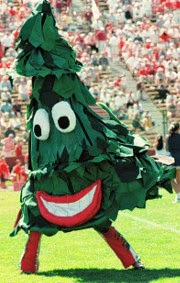
\includegraphics[width=1.75 cm]{stanford-tree.jpg}

\end{centering}

\end{frame}

\section{Introduction}

\begin{frame}
\frametitle{Congestion control!}

\begin{itemize}

\Large

\item Prevents congestion collapse

\item Allocates network resources among users

\item Can be purely end-to-end or not

\end{itemize}

\end{frame}

\begin{frame}
\frametitle{What's the right allocation?}
  \begin{centering}
    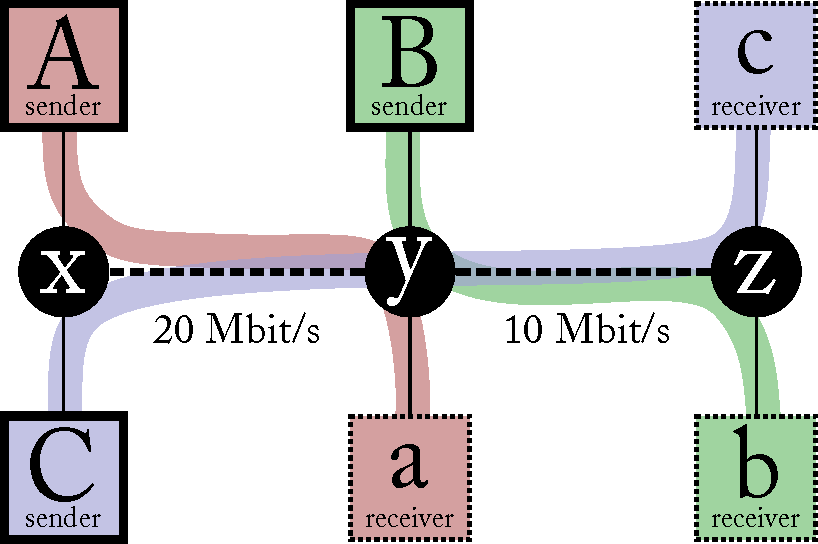
\includegraphics[width=3.75 in]{congestion-control-figure.pdf}

  \end{centering}
\end{frame}

\begin{frame}
\frametitle{What's the right allocation?}

  \begin{centering}
    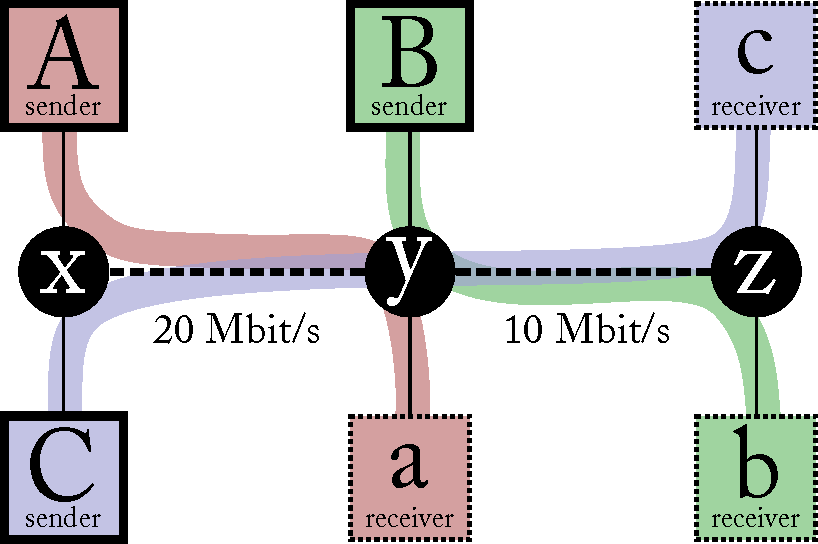
\includegraphics[width=1.9 in]{congestion-control-figure.pdf}

    \vspace{\baselineskip}

    \begin{tabular}{ccc|cc|l}
      \bf A$\rightarrow$a & \bf B$\rightarrow$b & \bf C$\rightarrow$c & $xy$ & $yz$ & \bf total throughput \\
      \hline
      \pause
      20 & 10 & 0  & 20 & 10 & 30\textcolor{White}{.0} \it \textcolor{DarkBlue}{(max utilization; worst for C)}\\
      \pause
      10 &  0  & 10 & 20 & 10 & 20\textcolor{White}{.0} \it \textcolor{DarkBlue}{(best for C)} \\
      \pause
      0 &  0  & \only<-4>{20}\only<5->{\textcolor{DarkGray}{\sout{20}}}\visible<5->{ 10} & 20 & 10 & \visible<5->{10\textcolor{White}{.0} \it \textcolor{DarkBlue}{(C floods; lots of drops at $y$)}} \\
      \pause
      15 & 5  & 5  & 20 & 10 & 25\textcolor{White}{.0} \it \textcolor{DarkBlue}{(max-min fairness)} \\
      \pause
      15.8 & 5.8 & 4.2 & 20 & 10 & 25.8 \it \textcolor{DarkBlue}{(proportional fairness)} \\
    \end{tabular}
    
  \end{centering}

\end{frame}

\begin{frame}
  \frametitle{TCP (simplified)}

\large
  
  \begin{itemize}
  \item Packets outstanding $\le$ \emph{congestion window} (\texttt{cwnd})
  \item[]
  \item \textbf{Initially}: $\texttt{cwnd} \leftarrow 3$
  \item \textbf{If} all \texttt{cwnd} packets received: $\texttt{cwnd} = \texttt{cwnd} + 1$
  \item \textbf{Else}: $\texttt{cwnd} = \texttt{cwnd} / 2$
  \end{itemize}
\end{frame}

\begin{frame}
\frametitle{The march of congestion-control protocols}
\only<1>{\noindent \hspace{-.75 cm} 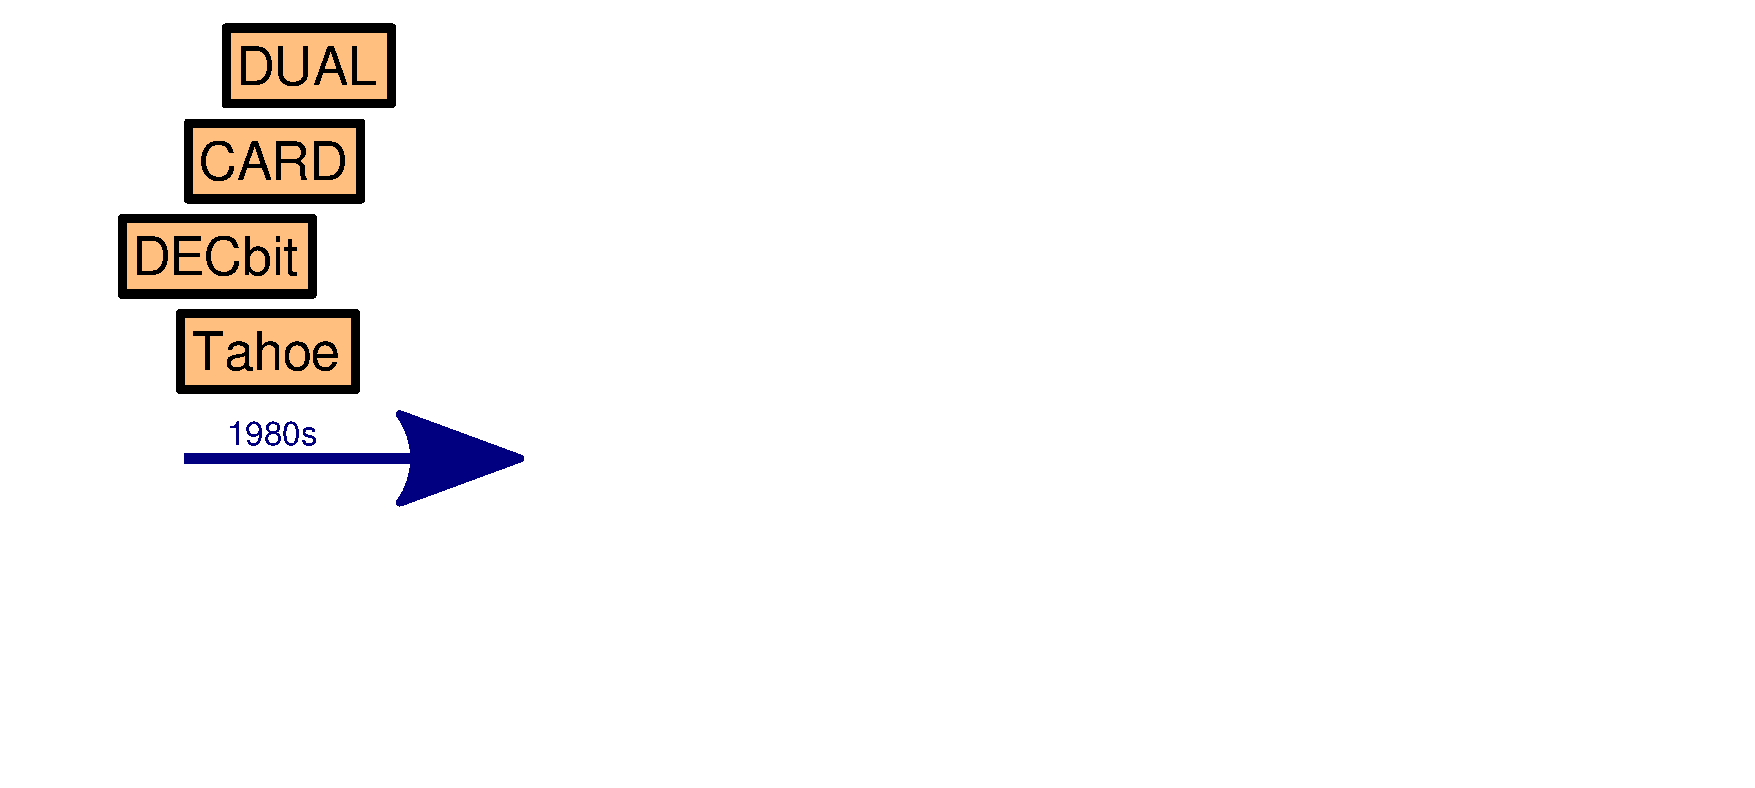
\includegraphics[width=1.1\textwidth]{march2-1.pdf}

}
\only<2>{\noindent \hspace{-.75 cm} 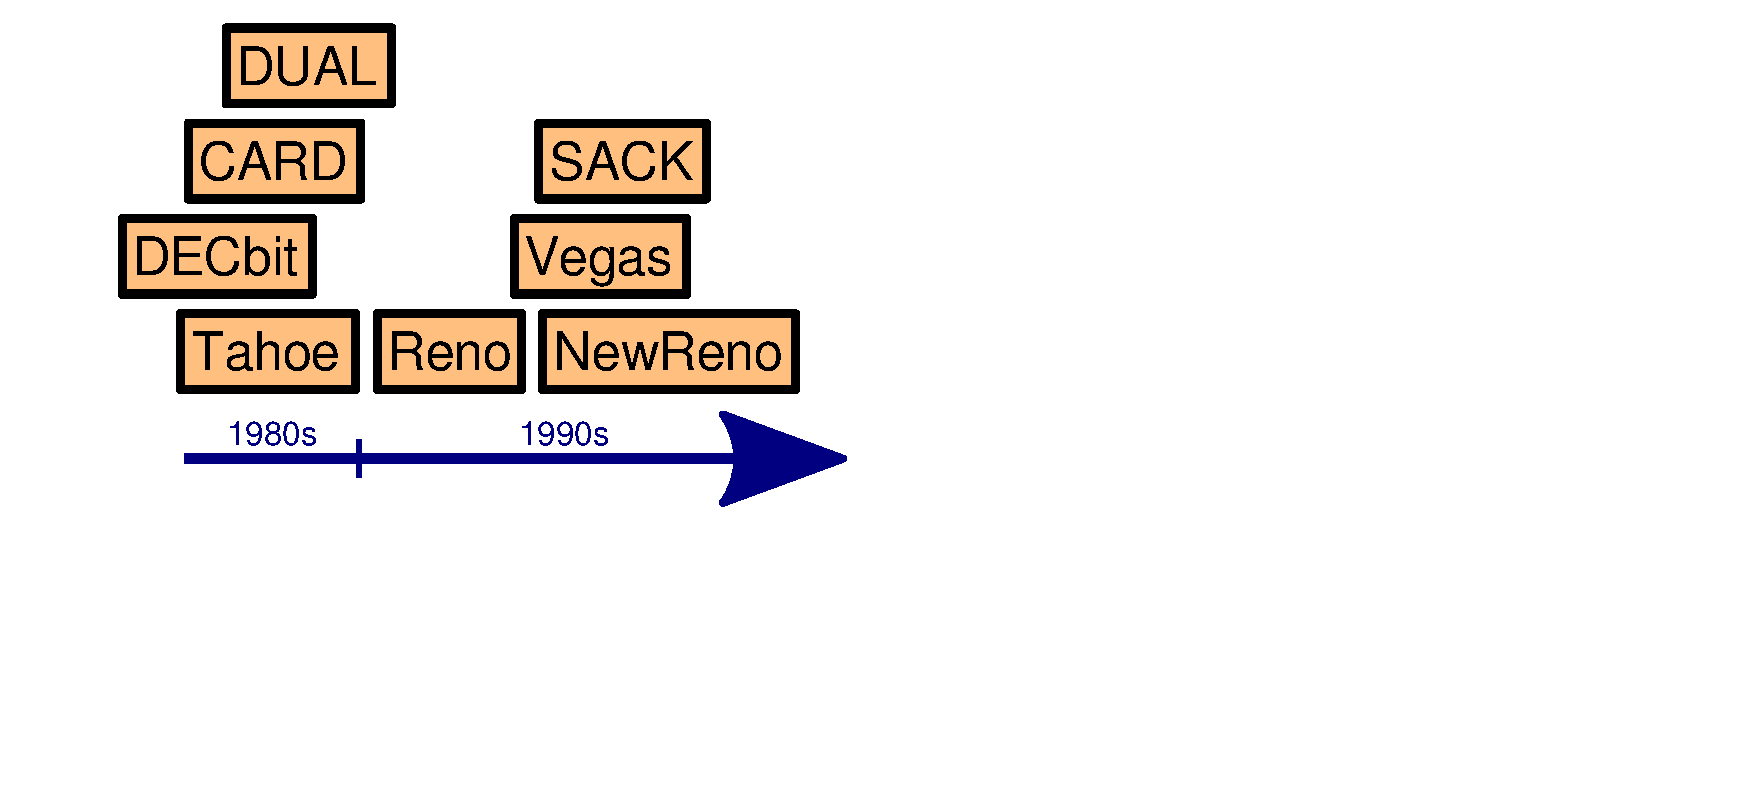
\includegraphics[width=1.1\textwidth]{march2-2.pdf}

}
\only<3>{\noindent \hspace{-.75 cm} 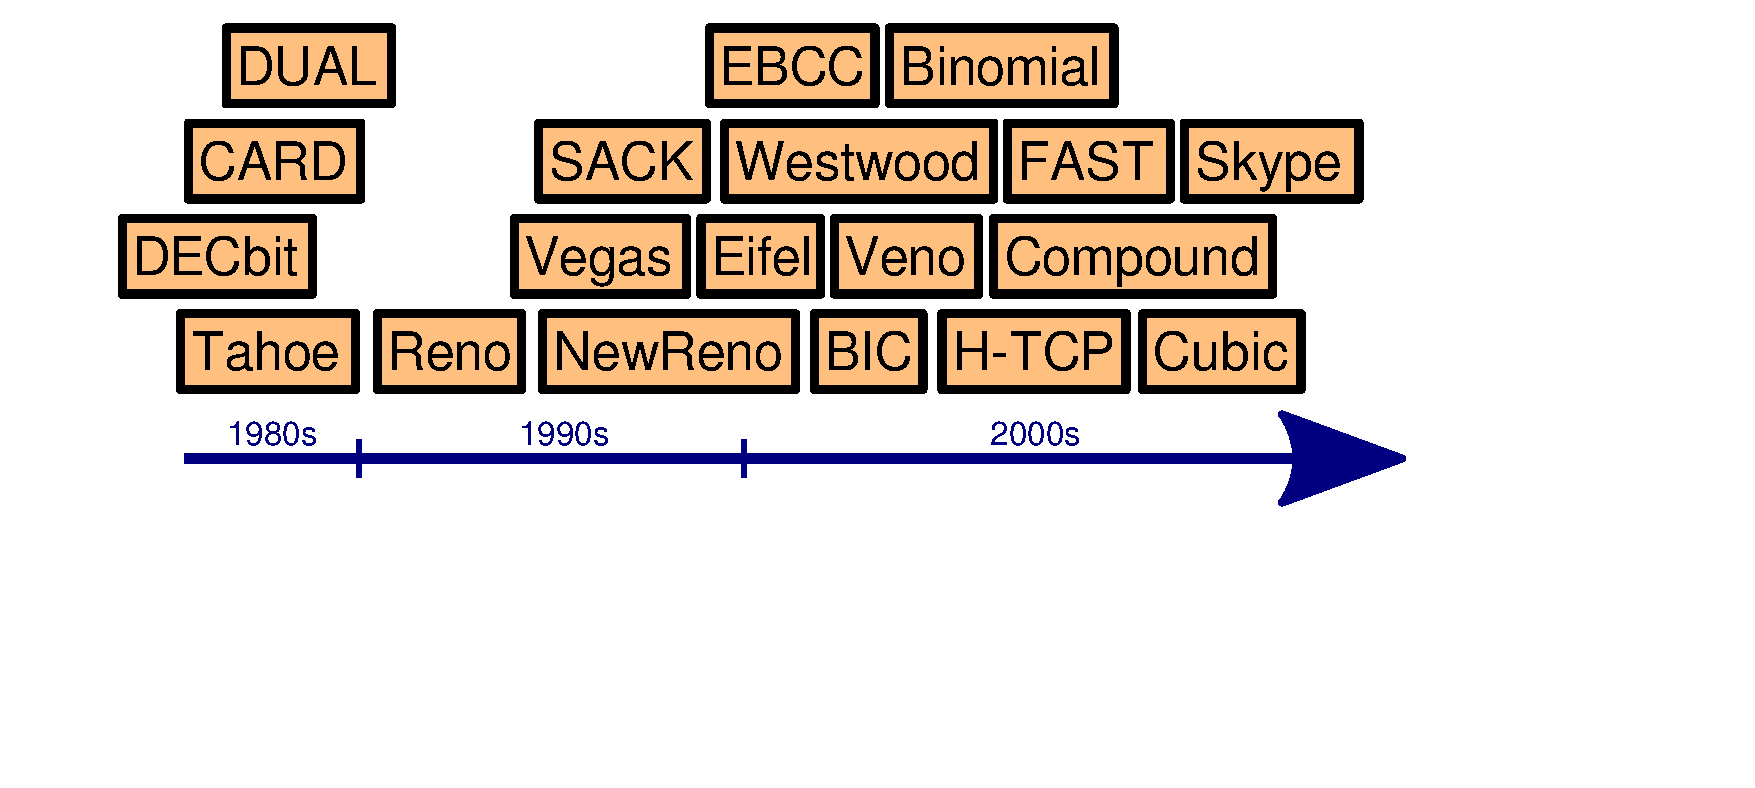
\includegraphics[width=1.1\textwidth]{march2-3.pdf}

}
\only<4>{\noindent \hspace{-.75 cm} 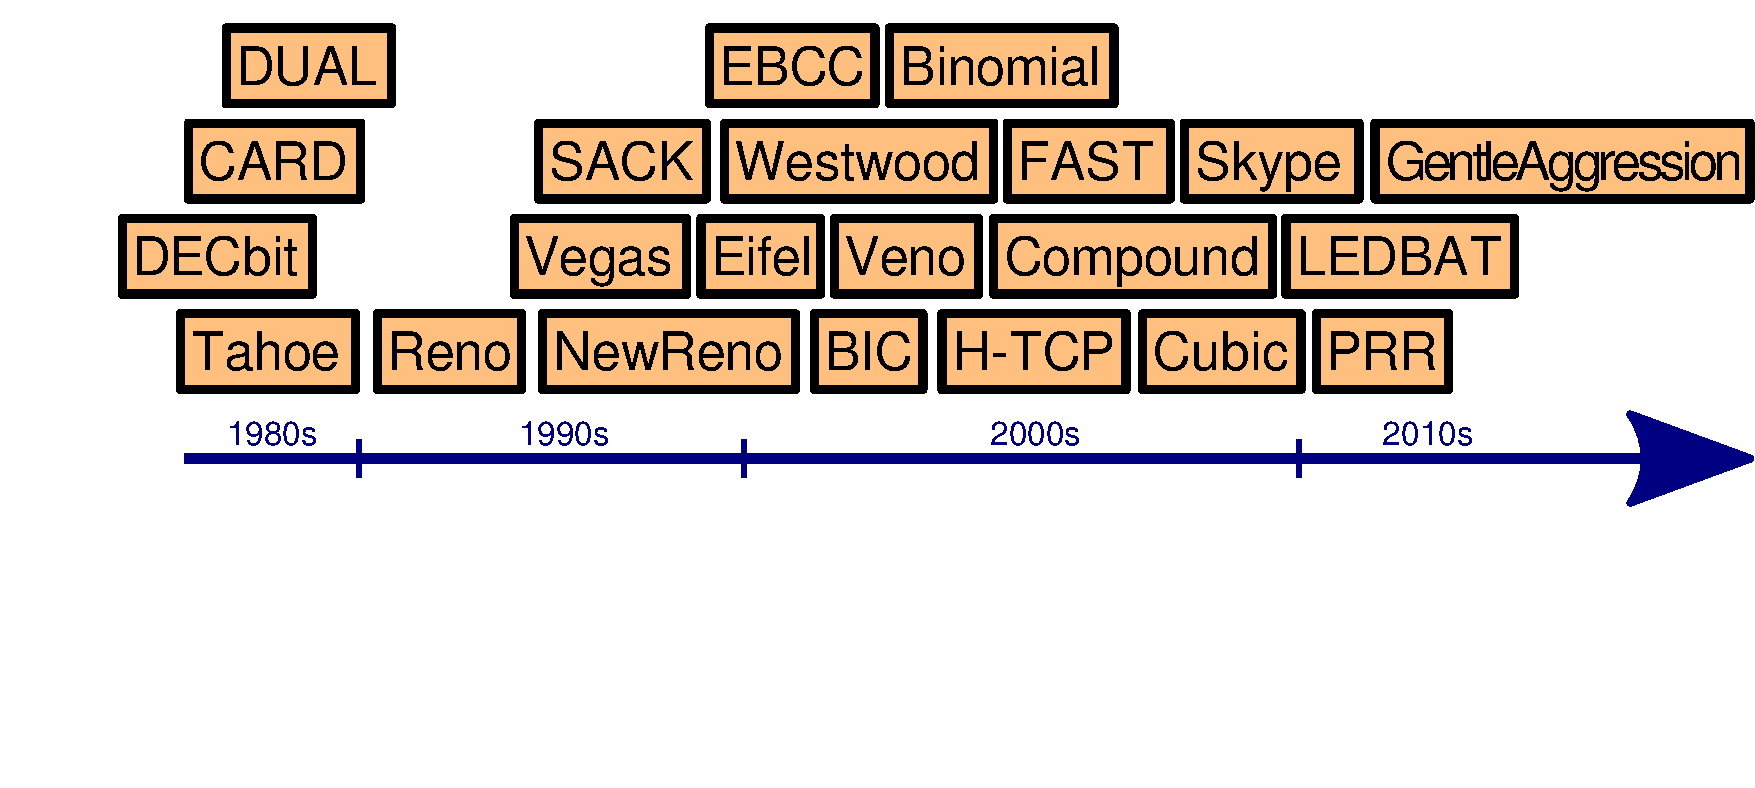
\includegraphics[width=1.1\textwidth]{march2-4.pdf}

}
\only<5>{\noindent \hspace{-.75 cm} 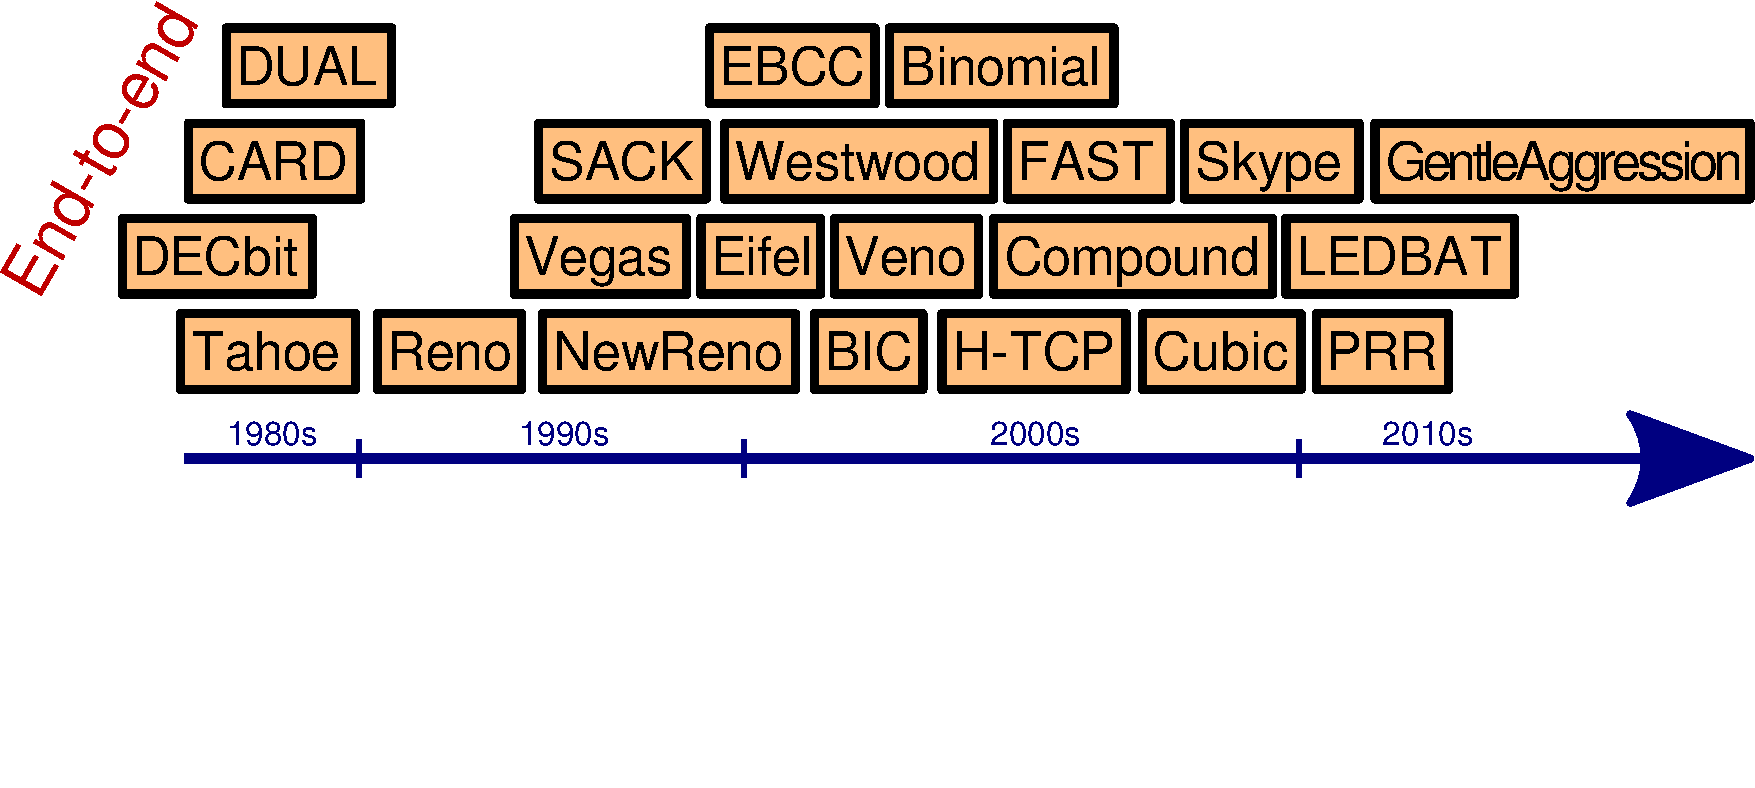
\includegraphics[width=1.1\textwidth]{march2-5b.pdf}

}
\only<6>{\noindent \hspace{-.75 cm} 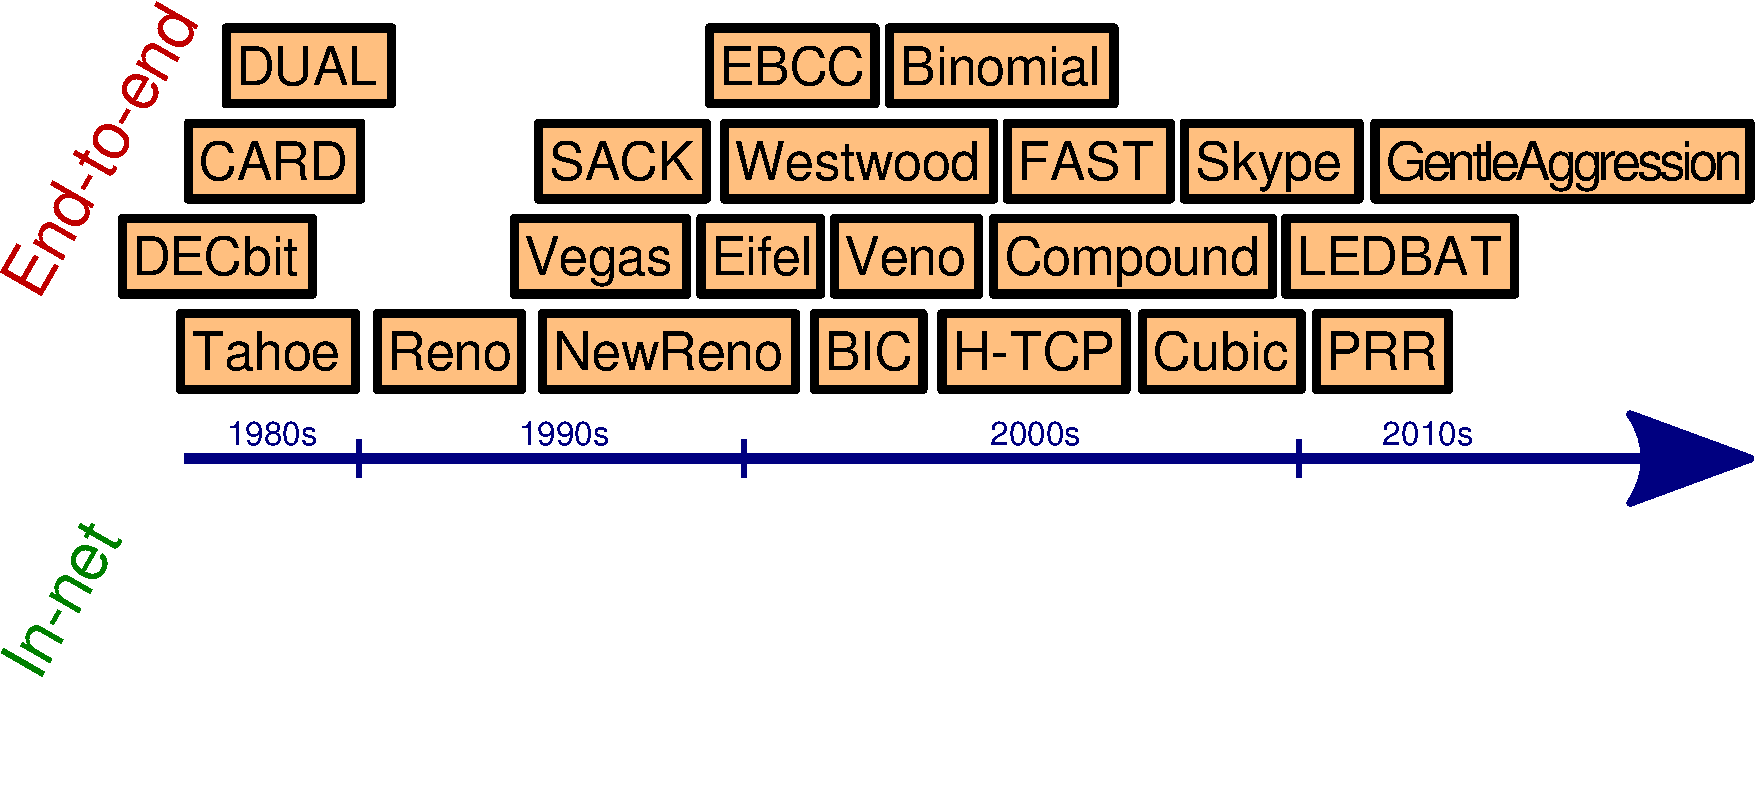
\includegraphics[width=1.1\textwidth]{march2-5.pdf}

}
\only<7>{\noindent \hspace{-.75 cm} 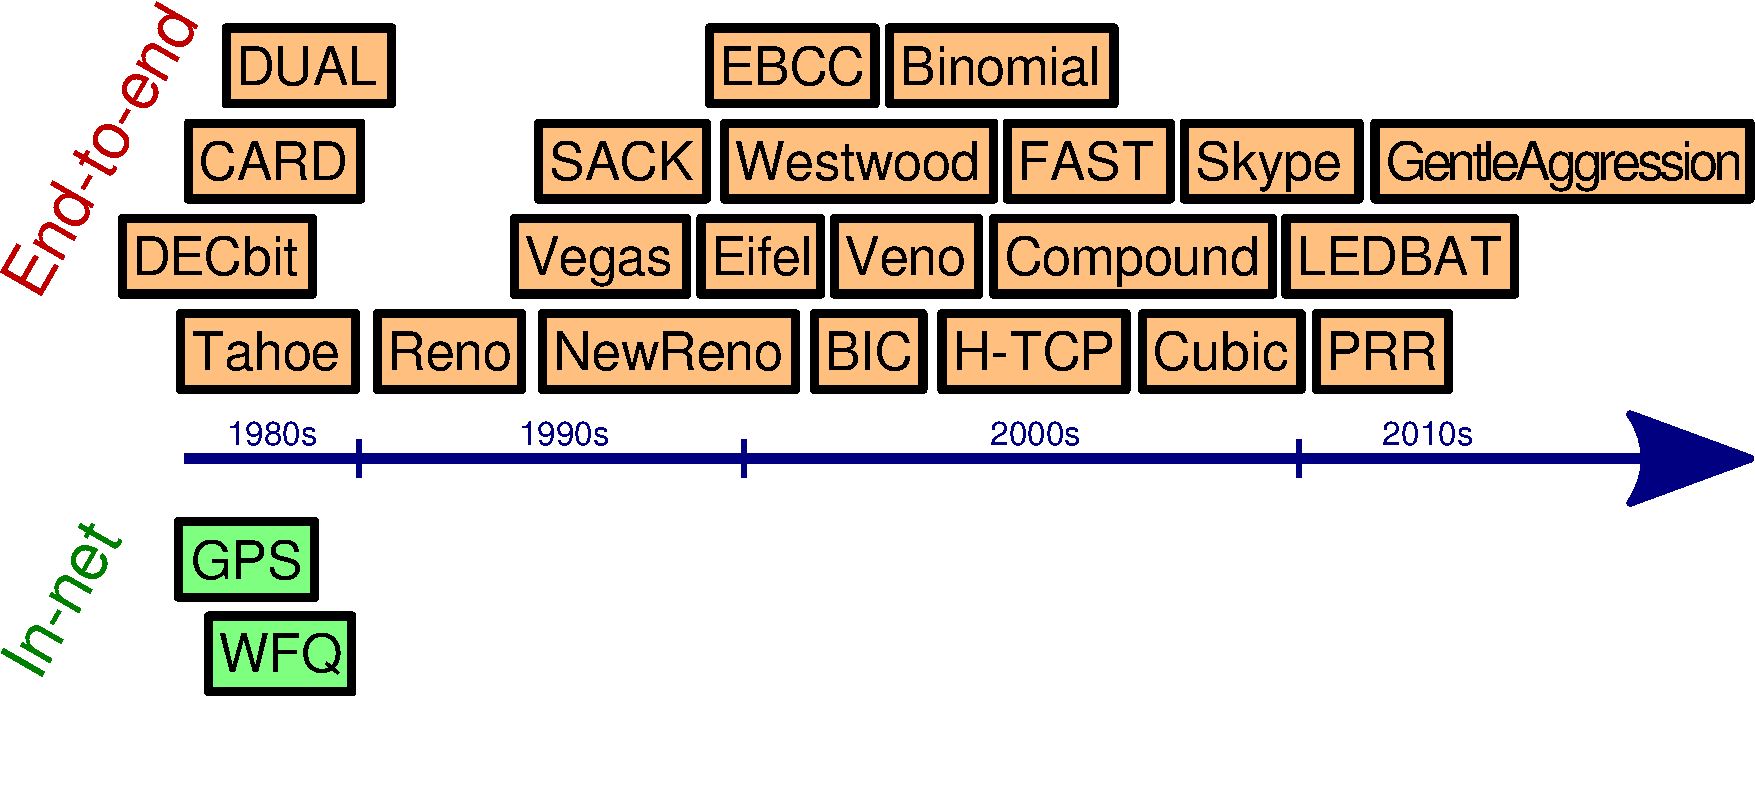
\includegraphics[width=1.1\textwidth]{march2-6.pdf}

}
\only<8>{\noindent \hspace{-.75 cm} 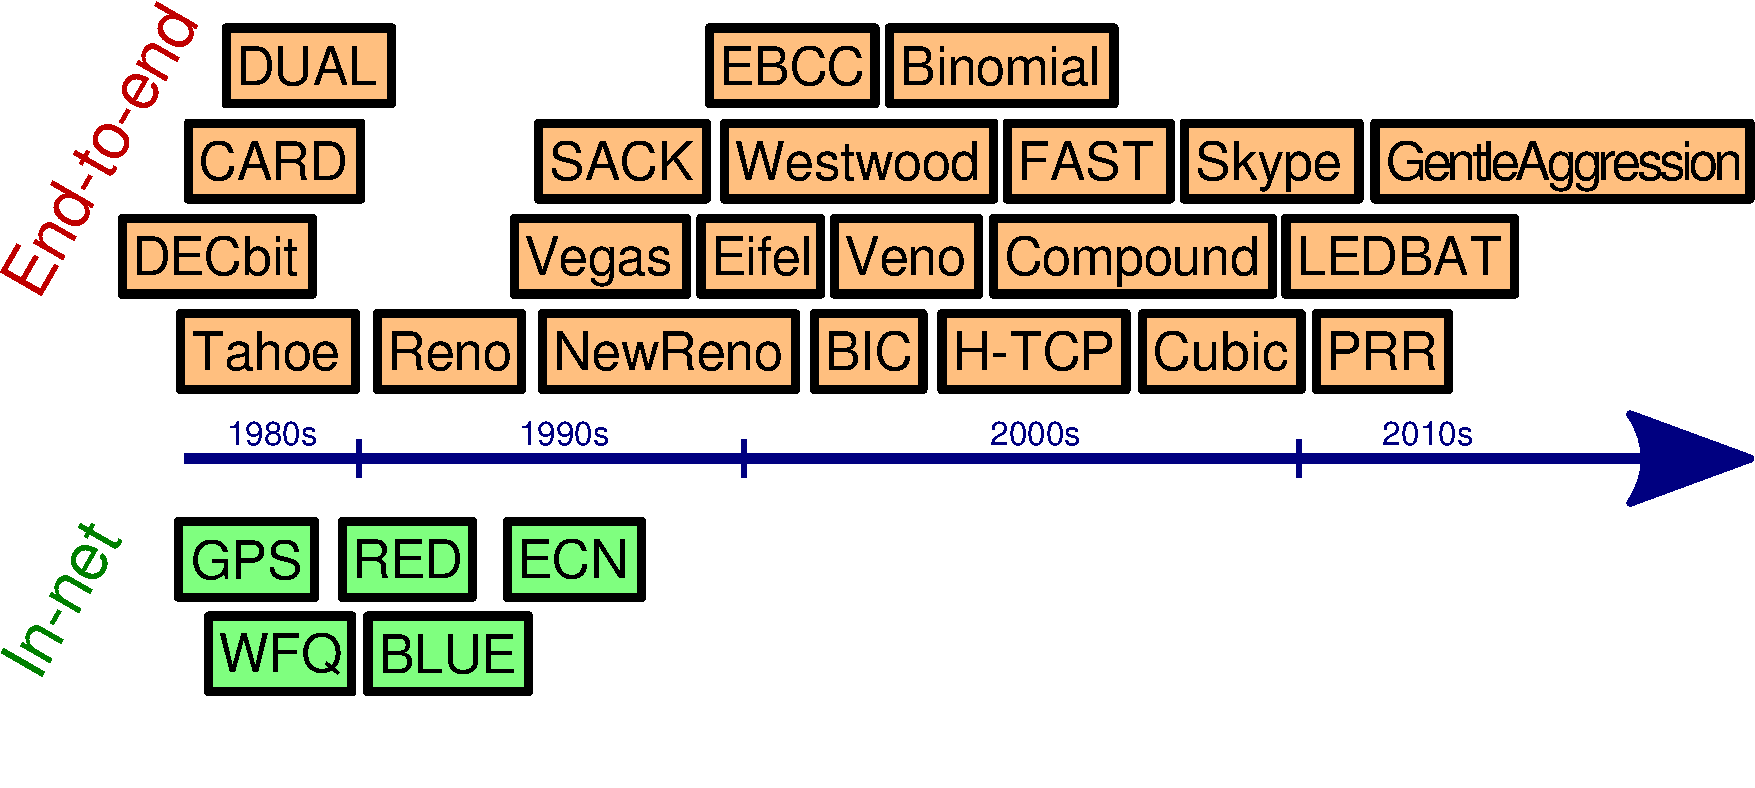
\includegraphics[width=1.1\textwidth]{march2-7.pdf}

}
\only<9>{\noindent \hspace{-.75 cm} 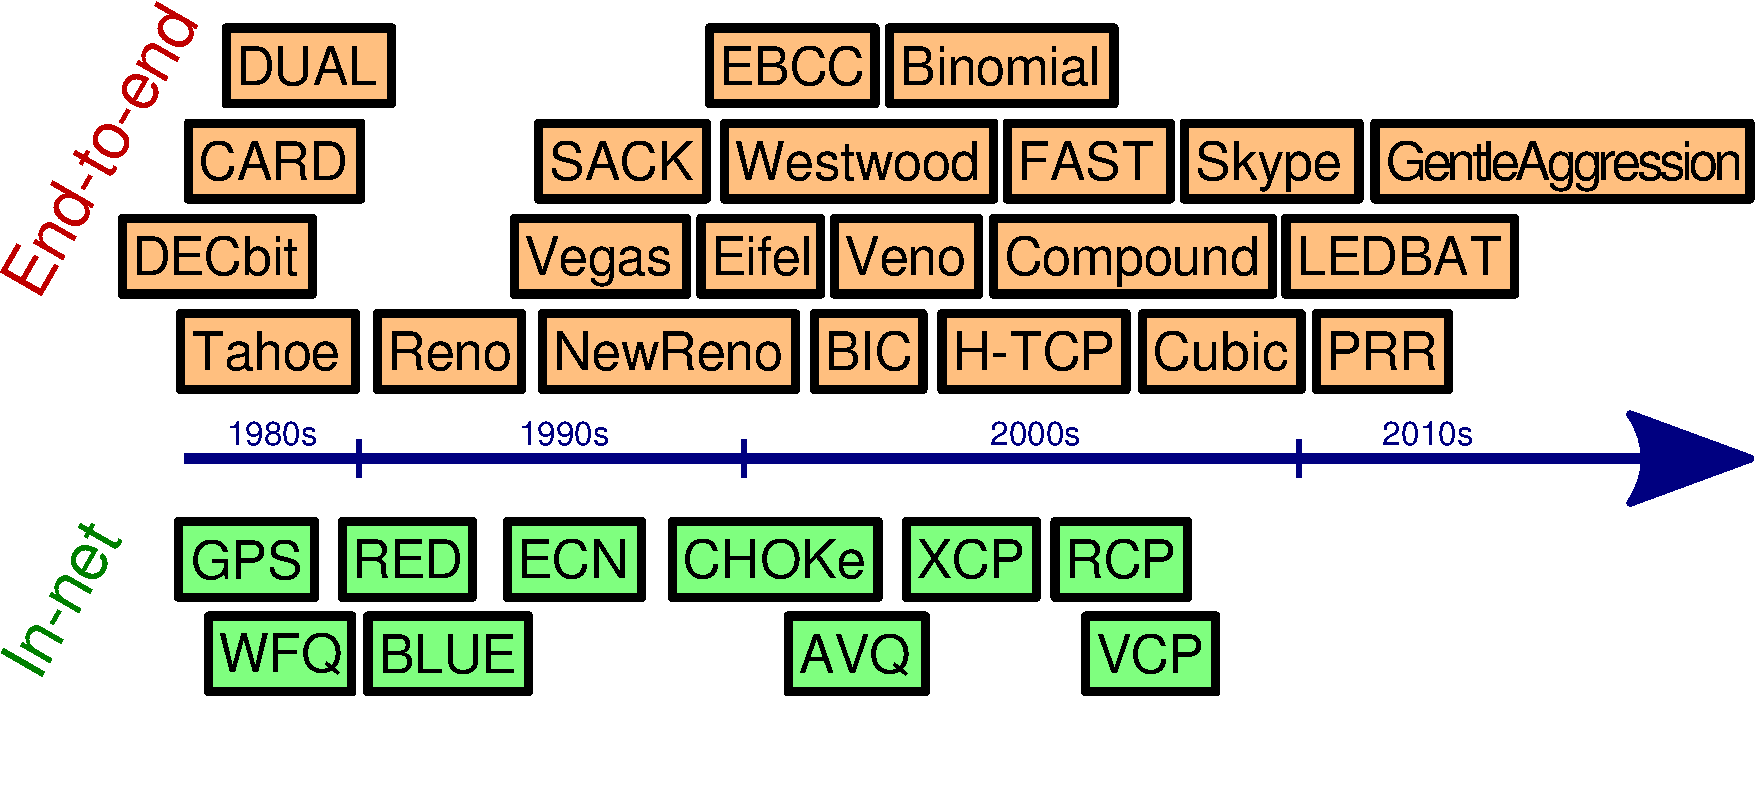
\includegraphics[width=1.1\textwidth]{march2-8.pdf}

}
\only<10>{\noindent \hspace{-.75 cm} 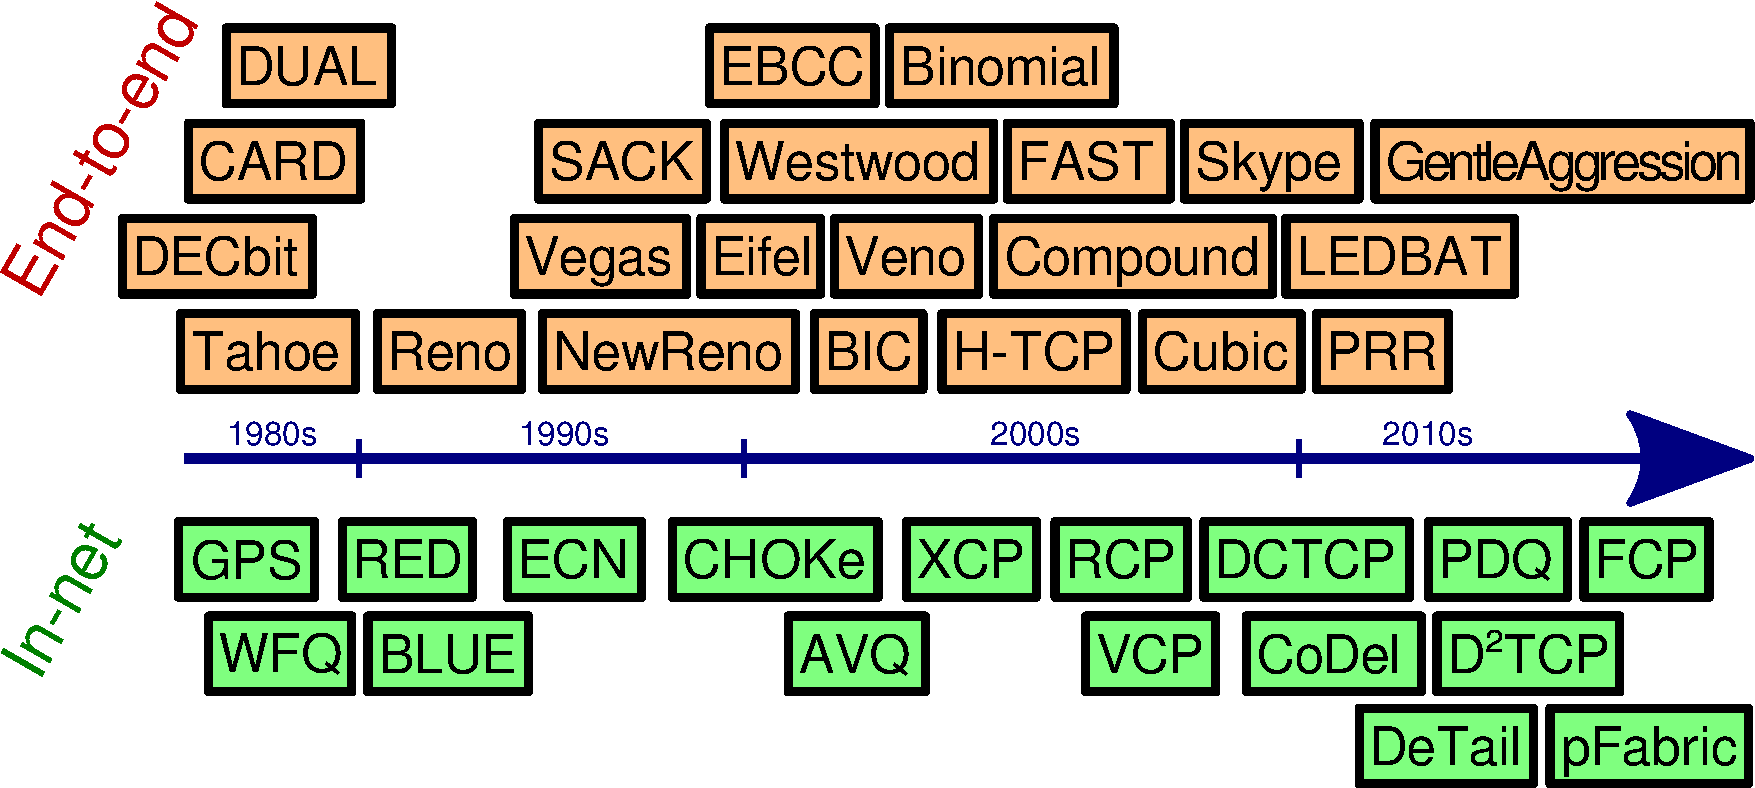
\includegraphics[width=1.1\textwidth]{march2-9.pdf}

}
\end{frame}

%\begin{frame}
%\begin{centering}
%\LARGE One size does not fit all.
%
%\end{centering}
%\end{frame}

\begin{frame}

\frametitle{Our work}

\begin{centering}

\LARGE \textcolor{DarkGreen}{If congestion control is the answer,\\what's the question?}

\vspace{\baselineskip}

\pause

\LARGE \textcolor{NavyBlue}{Are there better answers?}

\end{centering}

\end{frame}

\begin{frame}
\frametitle{Rational choice of scheme is challenging}

\begin{centering}

\includegraphics[height=20 pt]{cubic.pdf}\hspace{8 pt}{\bf vs.}\hspace{8 pt}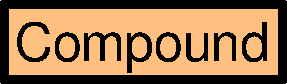
\includegraphics[height=20 pt]{compound.pdf}

\end{centering}

\ssline
\ssline
\ssline

\begin{itemize}

\Large

\item Different goals?

\item Different assumptions about network?

\item One scheme just plain better?

\end{itemize}

\end{frame}

%\begin{frame}
%\frametitle{What are the ends that TCP tries to achieve?}
%
%\begin{itemize}
%
%\Large
%
%\item ``Teleology of TCP'' is mostly unknown
%
%\item Asymptotic solutions for long-running flows
%
%\item Dynamical behavior is complex
%
%\end{itemize}
%
%\end{frame}

\begin{frame}
\frametitle{Networks constrained by a fuzzy idea of TCP's assumptions}

\Large

On today's Internet:

\begin{columns}

\begin{column}{0.66\textwidth}

\begin{itemize}
\item Mask stochastic loss
\item[] \hspace{1 cm}$\rightarrow$ {\bf \textcolor{Maroon}{bufferbloat}}
%\item Bufferbloat

\item No out-of-order delivery
\item[] \hspace{1 cm}$\rightarrow$ {\bf \textcolor{Maroon}{no parallel routing}}
\end{itemize}

\end{column}

\begin{column}{0.33\textwidth}

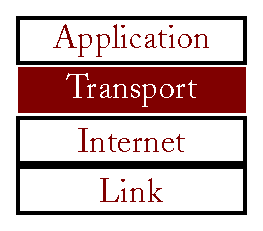
\includegraphics[width=\textwidth]{transport.pdf}

\end{column}

\end{columns}

\vspace{\baselineskip}

{\it Advice for Internet Subnetwork Designers}\\ (RFC 3819) is 21,000 words!

\end{frame}

\begin{frame}
\frametitle{Apps hack around TCP}

\Large

\begin{itemize}
\item Open lots of flows \hspace{1.9 cm} \only<2->{
\includegraphics[width=0.5cm]{firefox.png} \hspace{0.001 cm} 
\includegraphics[width=0.5cm]{chrome-64.png} \hspace{0.001 cm} 
\includegraphics[width=0.5cm]{Internet_Explorer_10_logo.png} \hspace{0.02 cm} 
\includegraphics[width=0.5cm]{safari.jpg} \hspace{0.02 cm} 
\includegraphics[width=0.5cm]{mozilladino.png}}

\item Goose slow start \only<3->{\hspace{2.18 cm} \raisebox{-0.6ex}{
\includegraphics[height=14 pt]{Google_Logo_Old.PNG}} \raisebox{-.125 ex}{
\includegraphics[height=10 pt]{mslogo.png}}}

\item Add pacing \hspace{3.3 cm} \only<4->{\raisebox{-.4 ex}{
\includegraphics[height=14 pt]{youtube.png}}}

\item Give up and do it yourself

\visible<5>{
\small
\hspace{5.95 cm}\begin{minipage}{3.5 cm}
{\bf Chrome} \textcolor{DarkBlue}{(QUIC)} \\
{\bf BitTorrent} \textcolor{DarkBlue}{($\mu$TP)} \\
{\bf Mosh} \textcolor{DarkBlue}{(SSP)} \\
{\bf Aspera} \textcolor{DarkBlue}{(fasp)} \\
\end{minipage}
}

\end{itemize}

\end{frame}

\begin{frame}
\frametitle{\textbf{Idea}: computer-synthesized transport}

\Large Transport layer should adapt to \textbf{whatever}

\begin{columns}

\begin{column}{0.66 \textwidth}

\begin{itemize}
\item network may do (\textbf{\textcolor{DarkBlue}{model}})

\item application wants (\textbf{\textcolor{DarkGreen}{mission}})

\end{itemize}

\end{column}

\begin{column}{0.33\textwidth}

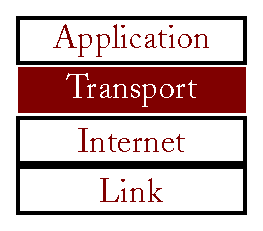
\includegraphics[width=\textwidth]{transport.pdf}

\end{column}

\end{columns}

\end{frame}

\begin{frame}
\frametitle{What we built}

\colorbox{Bisque}{
\begin{centering}
\noindent \begin{tabular}{ll}
\Large \textcolor{DarkRed}{\bf Remy}: & \Large a program that synthesizes \\ & \Large congestion-control schemes offline
\end{tabular}

\end{centering}}

\ssline
\ssline

\textcolor{DarkBlue}{\bf Input:}

\begin{itemize}
\item Assumptions about network and workload (\textbf{\textcolor{DarkBlue}{model}})

\item Application's objective (\textbf{\textcolor{DarkGreen}{mission}})
\end{itemize}

\textcolor{DarkBlue}{\bf Output:} CC algorithm for a TCP sender \hspace{0.177 cm}\textcolor{DarkBlue}{(RemyCC)}

\ssline

\textcolor{DarkBlue}{\bf Time:} hours to days

\vspace{\baselineskip}
\vspace{\baselineskip}
\vspace{\baselineskip}

\scriptsize

%KW and Hari Balakrishnan, \textbf{TCP ex Machina: Computer-Generated Congestion Control}, \textit{SIGCOMM 2013}

\end{frame}

\begin{frame}
\frametitle{The basic question of congestion control}

\section{The problem}

\begin{centering}
\fbox{
\begin{minipage}{6 cm}
\LARGE At this moment, do I:

\begin{itemize}

\item send a packet
\item not send a packet?

\end{itemize}

\end{minipage}
}

\end{centering}

\end{frame}

%\begin{frame}
%\frametitle{The goal}
%
%\Large
%
%\begin{itemize}
%
%\item Tradeoff between \textbf{efficiency} and \textbf{fairness}
%
%\item Tradeoff between \textbf{throughput} and \textbf{delay}
%
%\end{itemize}
%
%\end{frame}

\begin{frame}
\frametitle{Objectives of congestion control}

\textbf{Maximize}

\begin{itemize}

\item \begin{minipage}{3.75 cm}
\[\sum_i \log \left[ \textsf{throughput}_i \right]\]
\end{minipage} \textsf{\textcolor{DarkBlue}{(proportionally fair throughput)}}

\pause

\item
\begin{minipage}{3.75 cm}
\begin{tabular}{l}
\cellcolor{Bisque}\raisebox{0.75 cm}{\begin{minipage}{3.75 cm}
\[\sum_i \log \left[ \frac{\textsf{throughput}_i}{\visible<3->{
\textcolor{DarkBlue}{\big(}
}\textsf{delay}_i\visible<3->{
\textcolor{DarkBlue}{\big)^{\bm \delta}}}} \right]\]
\end{minipage} \textsf{\textcolor{DarkBlue}{(proportionally fair throughput/delay)}}}
\end{tabular}
\end{minipage}

\visible<4>{

\item \begin{minipage}{3.75 cm}
$\min_i \textsf{throughput}_i$
\end{minipage} \textsf{\textcolor{DarkBlue}{(max-min throughput)}}
}
\end{itemize}

\visible<4>{
\textbf{Minimize}

\begin{itemize}
\item average flow completion time

\item page load time

\item tail completion time

\end{itemize}
}

\end{frame}

\begin{frame}
\frametitle{Prior assumptions}

\begin{itemize}

\Large

\item Model of network uncertainty

\begin{itemize}
\item Link speed distribution
\item Delay distribution
\end{itemize}

\item Traffic model

\begin{itemize}
\item Web browsing, MapReduce, videoconferencing
\end{itemize}

\end{itemize}

\end{frame}

\begin{frame}
\frametitle{Dumbbell network}

\only<1>{\noindent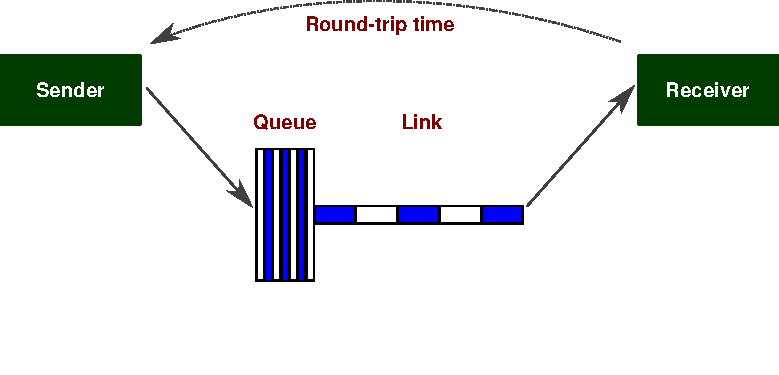
\includegraphics[width=\textwidth]{dumbbell-2.pdf}}\only<2>{\noindent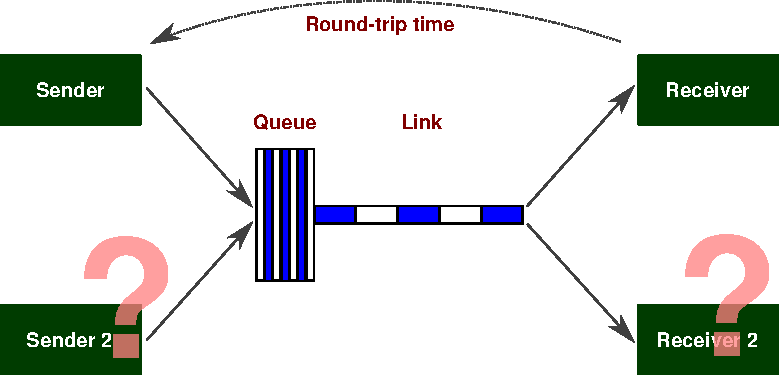
\includegraphics[width=\textwidth]{dumbbell-1.pdf}}\only<3>{\noindent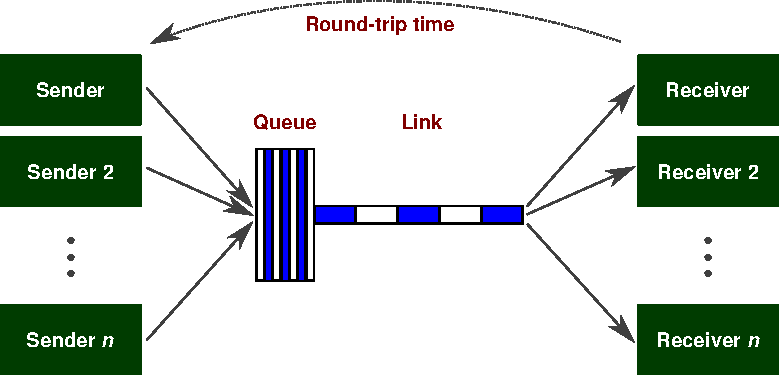
\includegraphics[width=\textwidth]{dumbbell.pdf}}

\end{frame}

%\begin{frame}
%\frametitle{Statement of the problem}
%
%\Large
%
%\begin{itemize}
%
%\item Endpoints have no control over routing
%
%\item Each sender only gets own receiver's acks
%
%\item Goal: \textbf{\textcolor{DarkBlue}{optimize expected value of objective}}
%
%\item[] \normalsize $\Rightarrow$ decentralized partially-observable Markov decision process
%
%\end{itemize}
%
%\end{frame}

\begin{frame}
\frametitle{Superrational congestion control}

\begin{centering}
\fbox{
\begin{minipage}{6 cm}
\LARGE At this moment,\textcolor{DarkBlue}{\bf *} do I:

\begin{itemize}

\item send a packet
\item not send a packet?

\end{itemize}

\end{minipage}
}

\ssline
\ssline
\ssline

\end{centering}

\Large \noindent \hspace{-.5cm} \mbox{\textcolor{DarkBlue}{\textbf{*} Assuming every node is running the same algorithm.}}

\end{frame}

\begin{frame}
\frametitle{Internet congestion control as a Dec-POMDP}

\begin{itemize}

\item[$I$:] independent endpoint computers

\pause

\item[$S$:] packets in net + whether each computer has data to send now

\pause

\item[$A_i$:] \{ send a packet, don't send a packet \}

\pause

\item[$\Omega$:] \mbox{acks from corresponding receiver ($O$ = deterministic)}

\pause

\item[$T$:] the \textbf{\textcolor{DarkBlue}{model}}

\pause

\item[$R$:] the \textbf{\textcolor{DarkGreen}{mission}}

\item[]

\item[] \fbox{\textcolor{DarkGreen}{\textbf{Complexity in general:}} undecidable}

\end{itemize}

\end{frame}

\begin{frame}
\frametitle{Remy: search for super\textcolor{Black}{rat}ionality}

\section{Remy}

\large

\begin{itemize}

\item Remy searches for the best congestion-control algorithm

\item[]

\item Optimizes expected objective over prior assumptions

\item[]

\item Makes tractable by \textcolor{DarkBlue}{limiting available state}

\end{itemize}

\end{frame}

\begin{frame}
\frametitle{A RemyCC tracks four congestion signals}

\large

\hspace{0.5 cm}\begin{minipage}{10.0 cm}
\begin{itemize}

\item[$rec\_rate_\alpha$:] \textcolor{Red}{\textit{``How fast are packets arriving (now)?''}}

\item[$rec\_rate_\beta$:] \textcolor{Red}{\textit{``How fast are packets arriving (smoothed)?''}}

\item[]

\item[$send\_rate$:] \textcolor{Red}{\textit{``How fast have I been sending?''}}

\item[]

\item[$rtt\_ratio$:] ratio of last RTT to smallest RTT so far

\textcolor{Red}{\textit{``How long is the queue?''}}

\end{itemize}
\end{minipage}

\end{frame}

\begin{frame}
\frametitle{Why these four features?}

\Large

\begin{itemize}

\item We can measure the benefit of each!

\item[]

\item Removing any one hurts

\begin{itemize}
\item losing $rec\_rate_\alpha$ hurts the most
\end{itemize}

\item[]

\item More signals increase search time

\item[]

\item[] \ldots but others might help on some networks

\end{itemize}

\end{frame}

\begin{frame}
\frametitle{A RemyCC maps each state to an action}

\Large

\[\textsc{RemyCC}( \textcolor{DarkBlue}{r\_ewma}, \textcolor{DarkBlue}{s\_ewma}, \textcolor{DarkBlue}{rtt\_ratio} ) \rightarrow \langle \textcolor{Red}{m}, \textcolor{Red}{b}, \textcolor{Red}{\tau} \rangle \]

\ssline
\ssline

\begin{tabular}{ll}

\textcolor{Red}{$m$} & Multiple to congestion window \\

\textcolor{Red}{$b$} & Increment to congestion window \\

\textcolor{Red}{$\tau$} & Minimum interval between two outgoing packets \\

\end{tabular}

\end{frame}

\begin{frame}
\frametitle{Runtime for a RemyCC}

\large

\textbf{On ack:}

\begin{itemize}
\item $\langle \textcolor{Red}{m}, \textcolor{Red}{b}, \textcolor{Red}{\tau}\rangle \leftarrow \textsc{RemyCC}( \textcolor{DarkBlue}{r\_ewma}, \textcolor{DarkBlue}{s\_ewma}, \textcolor{DarkBlue}{rtt\_ratio} )$

\item $\texttt{cwnd} \leftarrow \textcolor{Red}{m} \cdot \texttt{cwnd} + \textcolor{Red}{b}$
\end{itemize}

\textbf{Send packet if:}

\begin{itemize}
\item $\texttt{cwnd} > \texttt{FlightSize}$, and

\item last packet sent $> \textcolor{Red}{\tau}$ ago
\end{itemize}

\end{frame}

\begin{frame}
\frametitle{Remy's job}

\Large

\colorbox{Bisque}{
\begin{minipage}{\textwidth}
Find piecewise-continuous \textsc{RemyCC}() that \\ optimizes expected value of objective function

\end{minipage}}

\end{frame}

\begin{frame}
\frametitle{Remy example: 2D state space}

\large

\textbf{On ack:}

\vspace{\baselineskip}

\noindent \mbox{$\langle \textcolor{Red}{m}, \textcolor{Red}{b}, \textcolor{Red}{\tau}\rangle \leftarrow \textsc{\footnotesize RemyCC}( send\_rate, rec\_rate_{\alpha},\begin{tabular}{l}\only<2>{\cellcolor{DarkBlue}}\textcolor{DarkBlue}{$rec\_rate_{\beta}, rtt\_ratio$}\end{tabular} )$}

\end{frame}

\begin{frame}
\frametitle{Remy example: \textbf{\textcolor{DarkBlue}{model}}}

\large

\begin{tabular}{llll}
\bf Quantity & & \bf Distribution & \bf Units \\

\hline \\

Link speed & & Uniform(10, 20) & Mbps \\

\\

RTT & & Uniform(100, 200) & ms \\

\\

$n$ & & Uniform(1, 16) & how many flows? \\

\\

``On'' process & & $\mathrm{exp}[\mu = 5]$ & seconds \\

``Off'' process & & same \\

\end{tabular}

\end{frame}

\begin{frame}
\frametitle{Remy example: \textbf{\textcolor{DarkGreen}{mission}}}

\LARGE

\[\sum_i \log \left[ \frac{\textsf{throughput}_i}{\textsf{delay}_i} \right]\]

\end{frame}

\begin{frame}
\frametitle{Optimize default action}
\begin{centering}
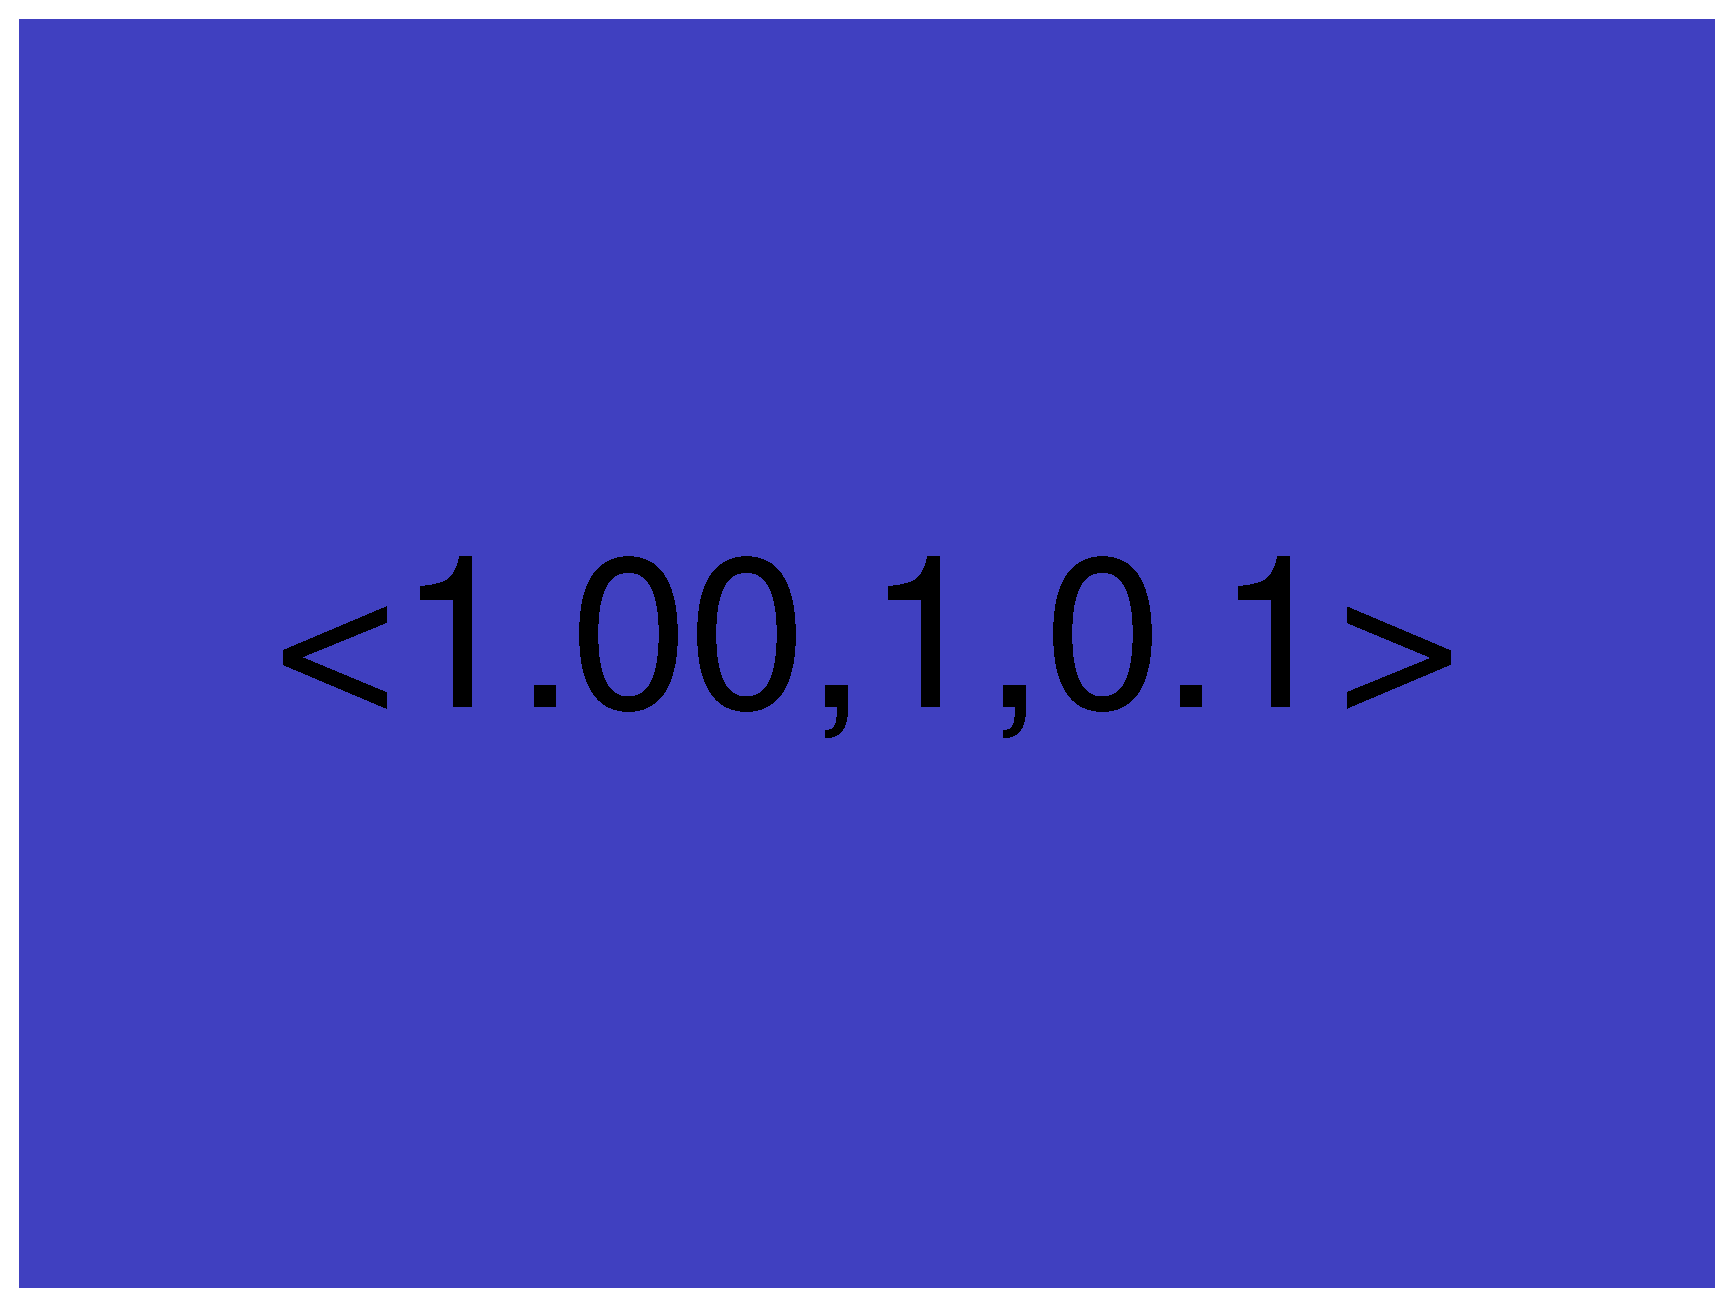
\includegraphics[width=8.5 cm]{remy-graph/graph/test0.pdf}

\end{centering}
\end{frame}

\begin{frame}
\frametitle{Split and duplicate at median query}
\begin{centering}
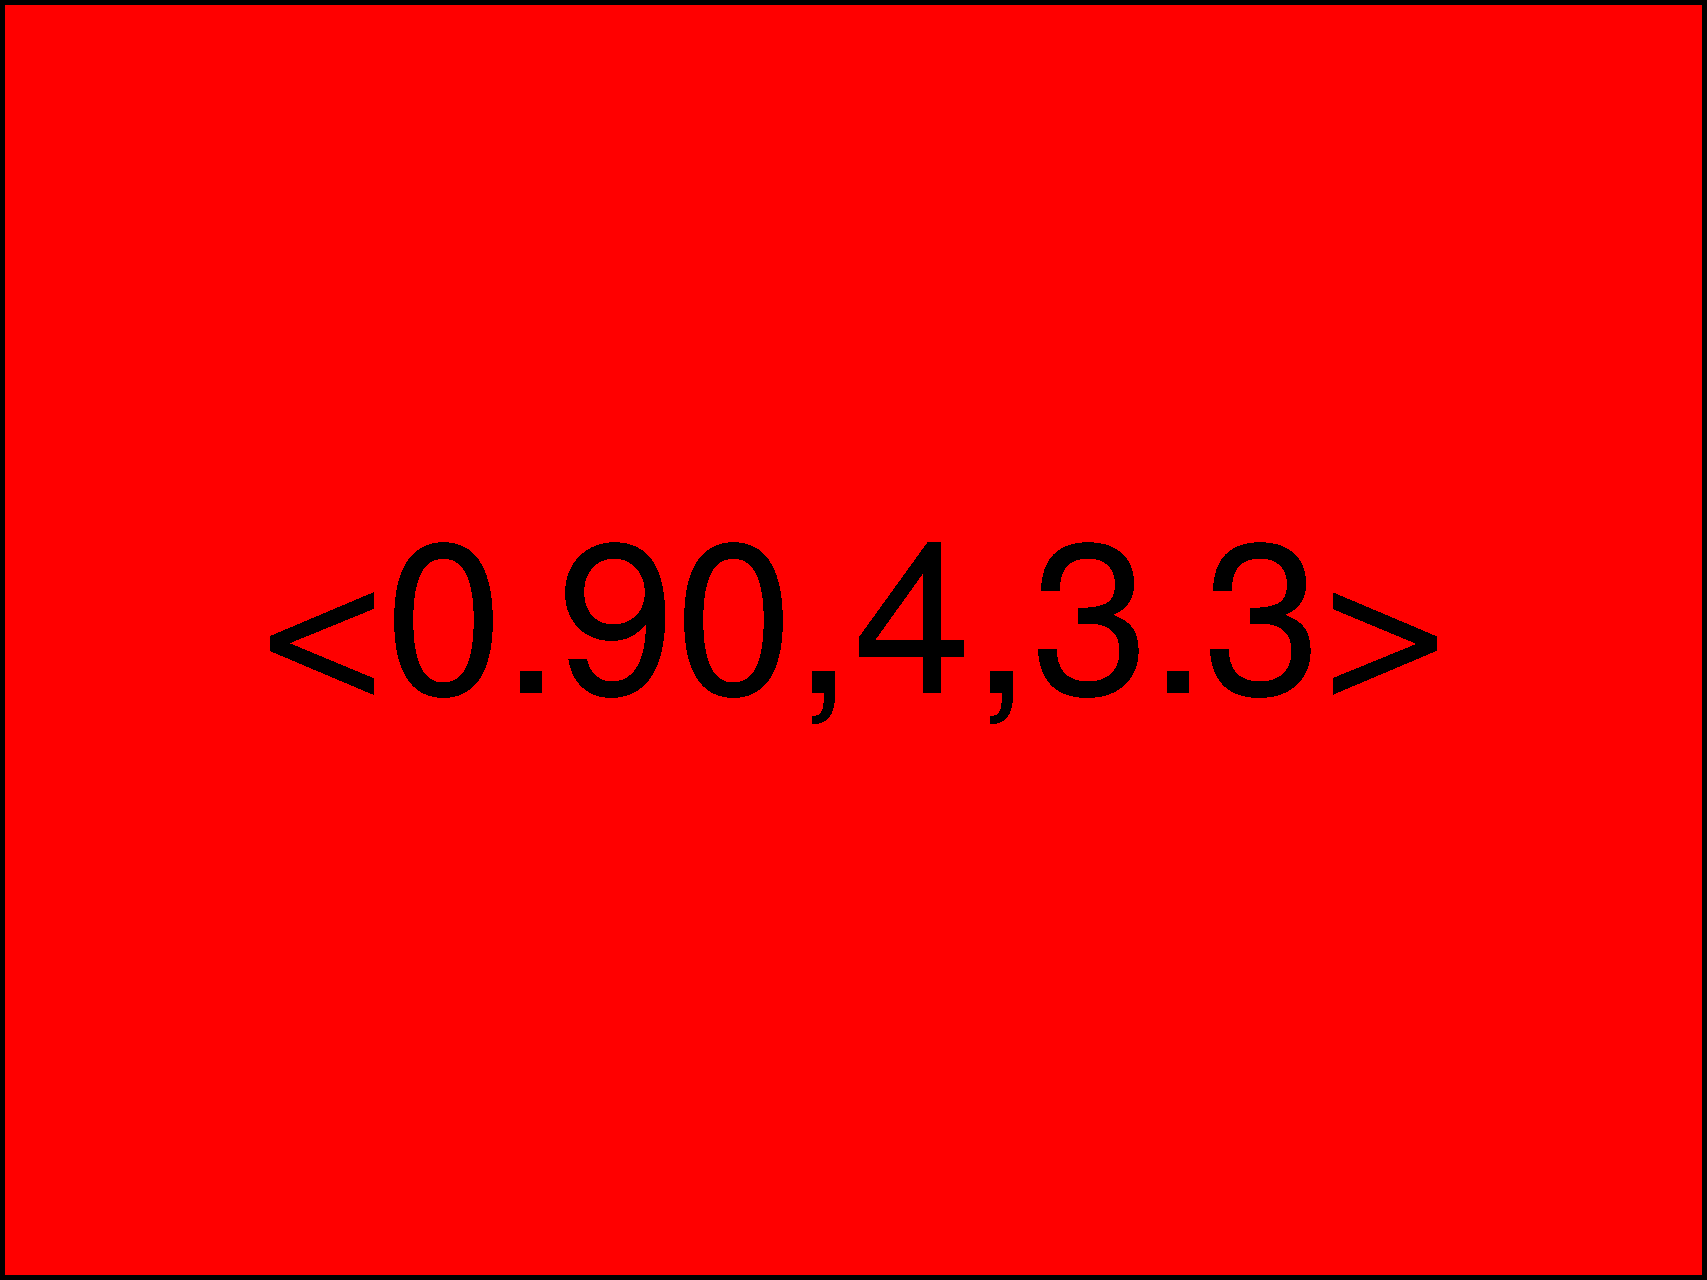
\includegraphics[width=8.5 cm]{remy-graph/graph/test1.pdf}

\end{centering}
\end{frame}

\begin{frame}
\frametitle{Run in simulation}
\begin{centering}
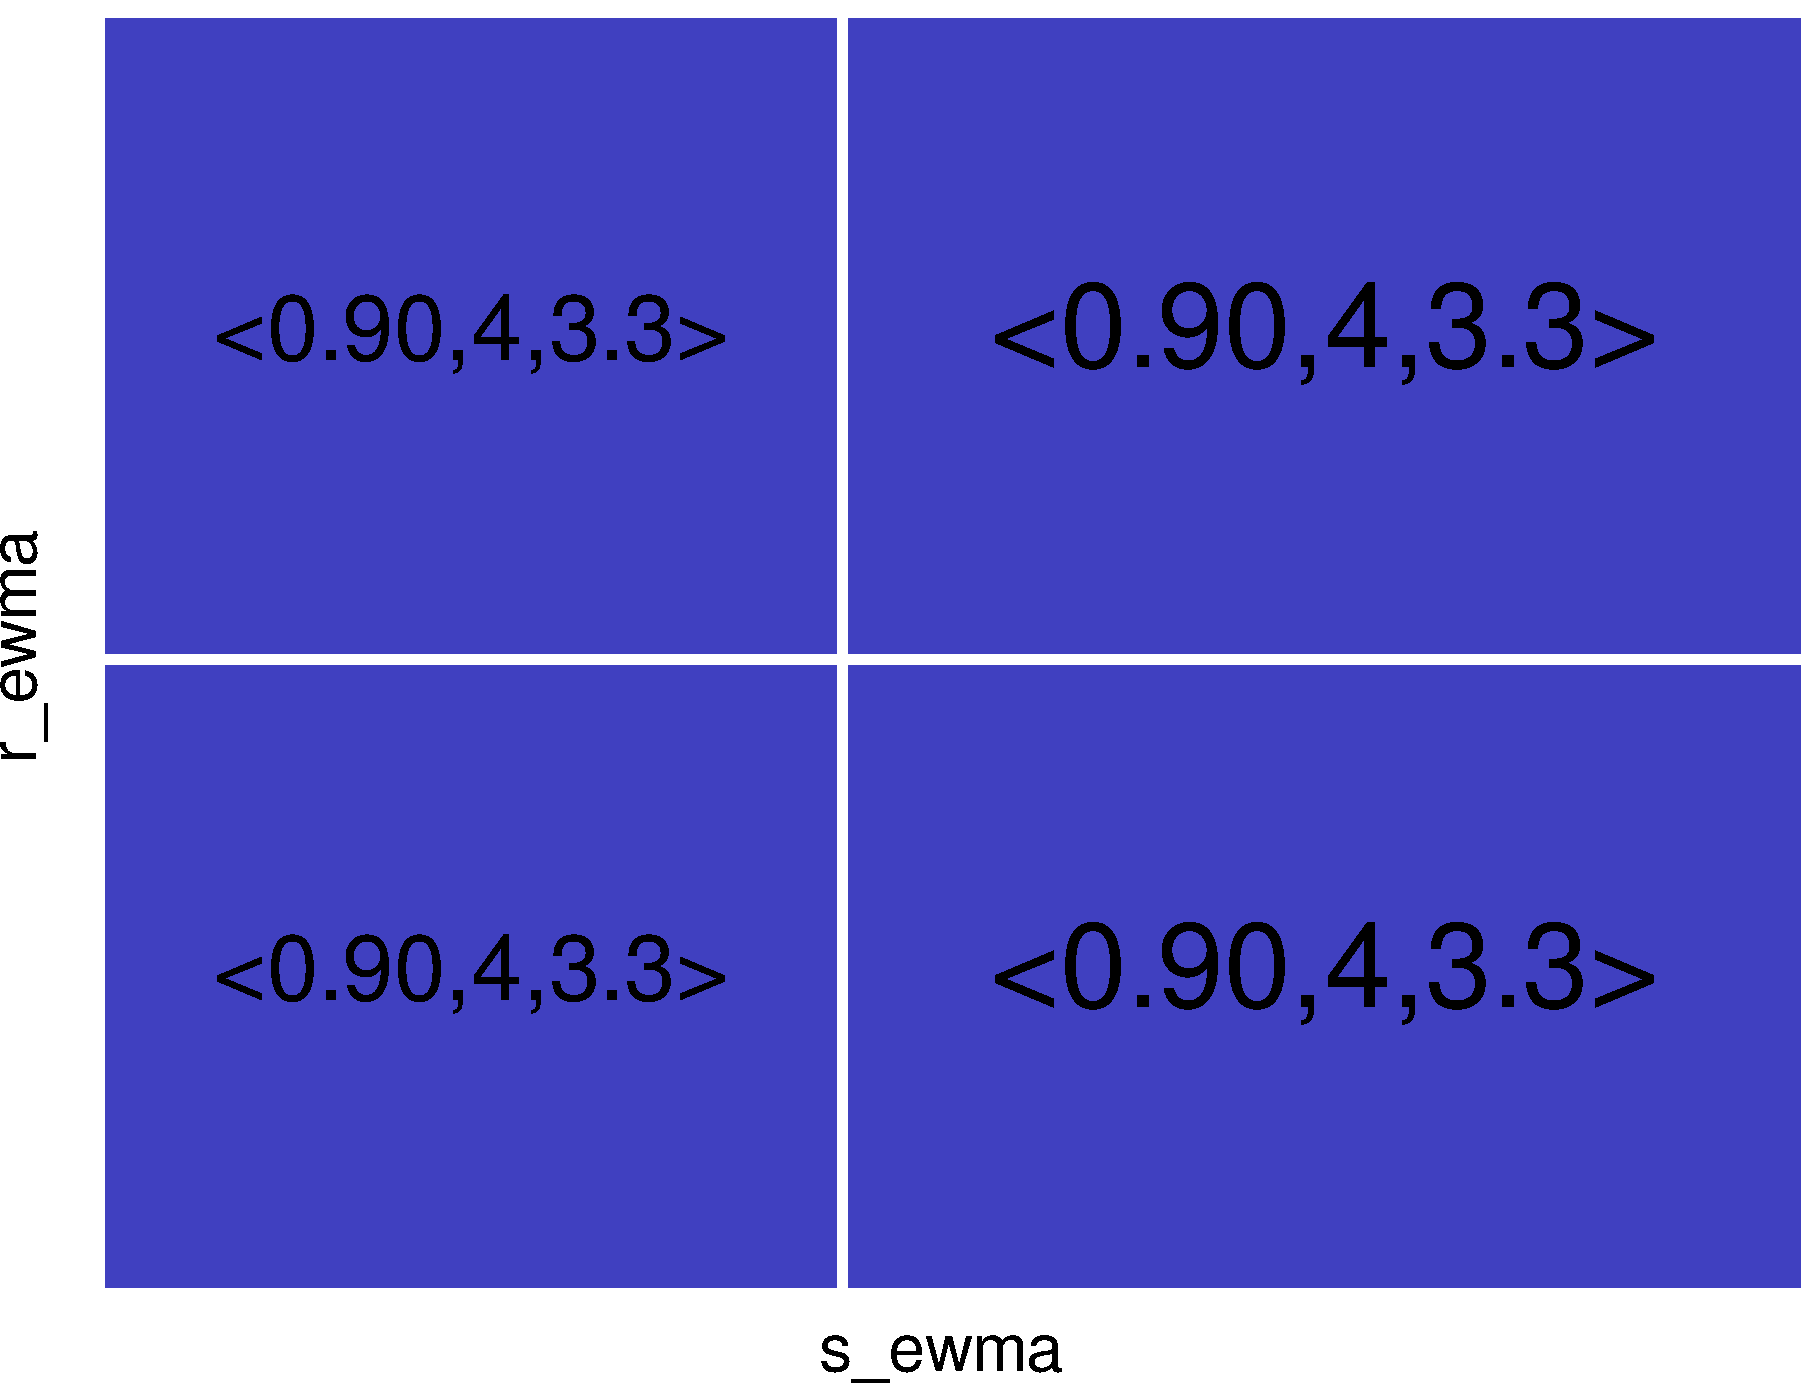
\includegraphics[width=8.5 cm]{remy-graph/graph/test2.pdf}

\end{centering}
\end{frame}

\begin{frame}
\frametitle{Optimize all actions}
\begin{centering}
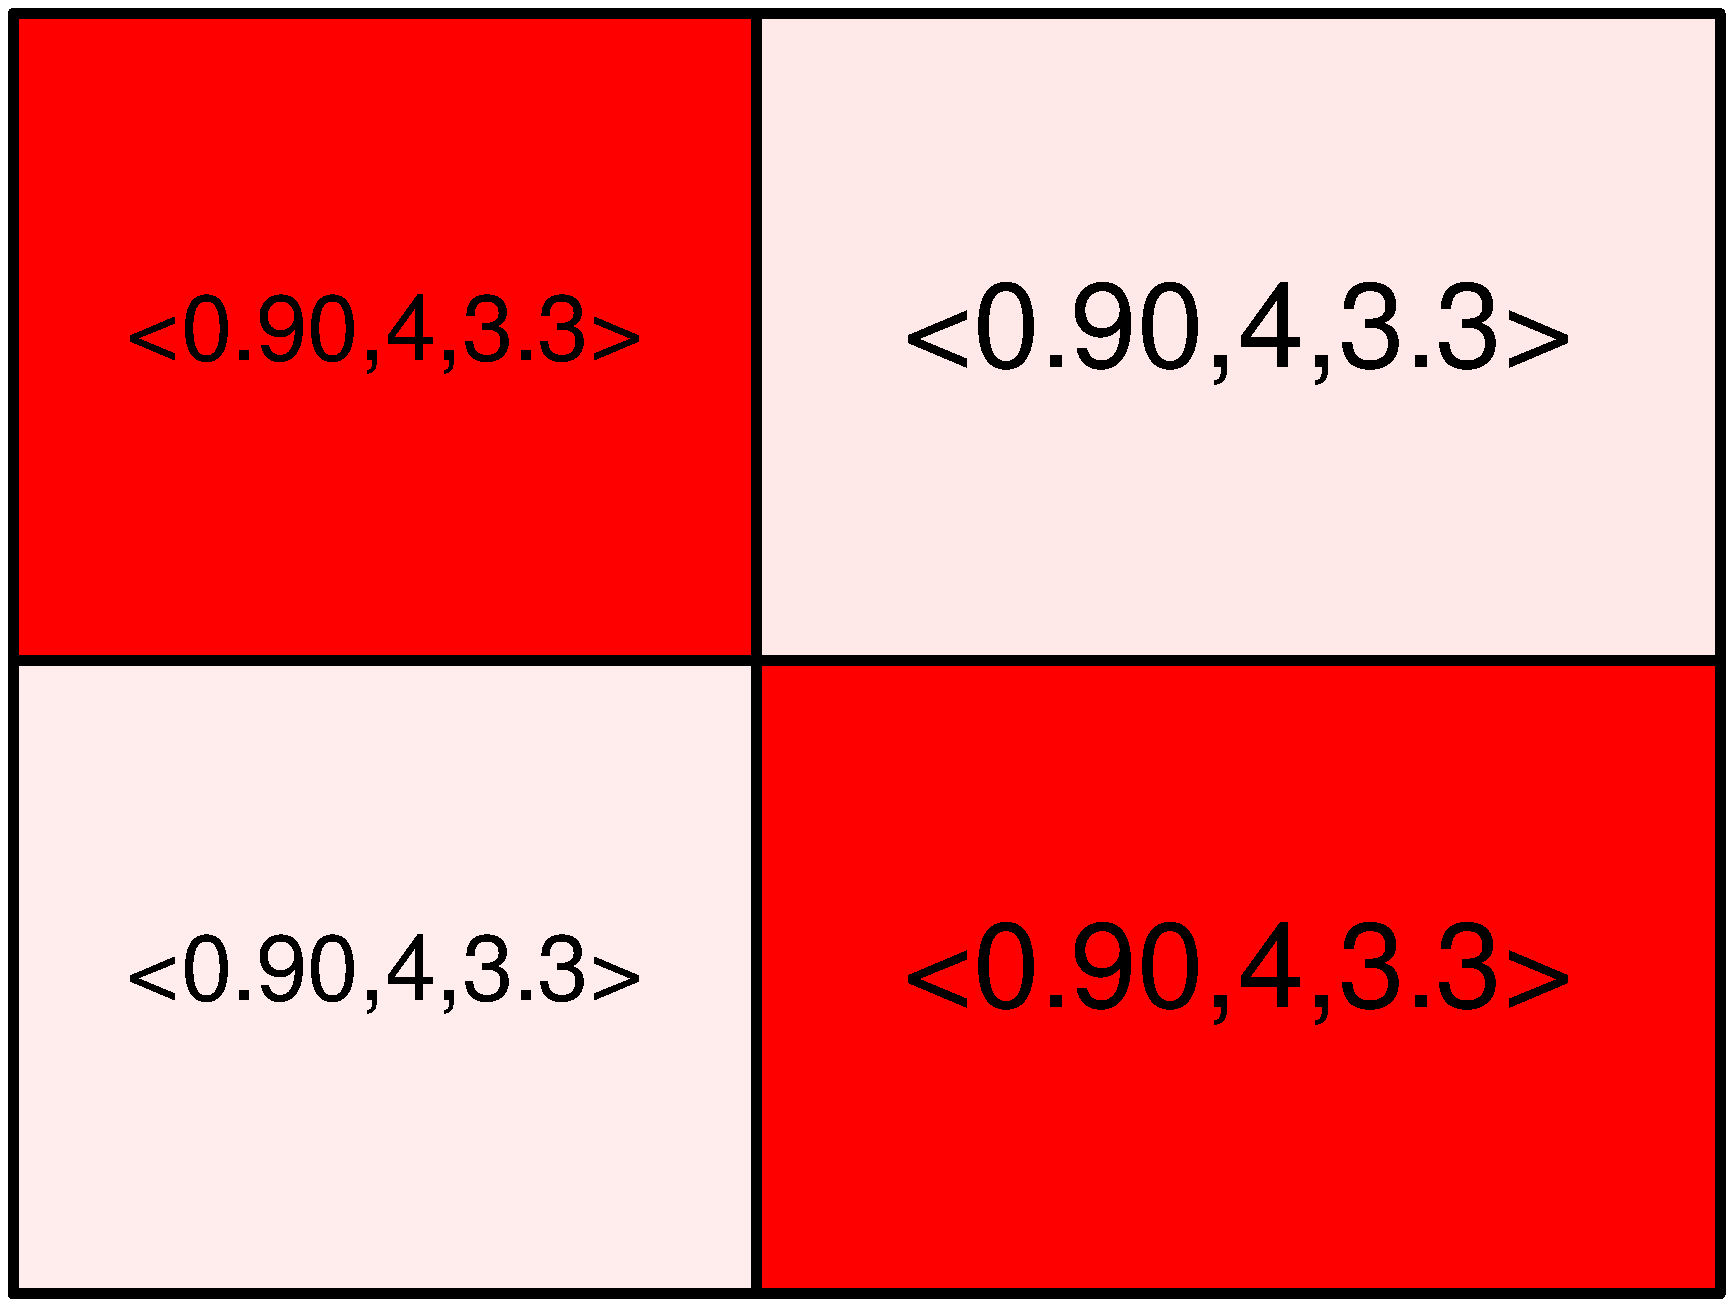
\includegraphics[width=8.5 cm]{remy-graph/graph/test3.pdf}

\end{centering}
\end{frame}

\begin{frame}
\frametitle{Split most-used rule}
\begin{centering}
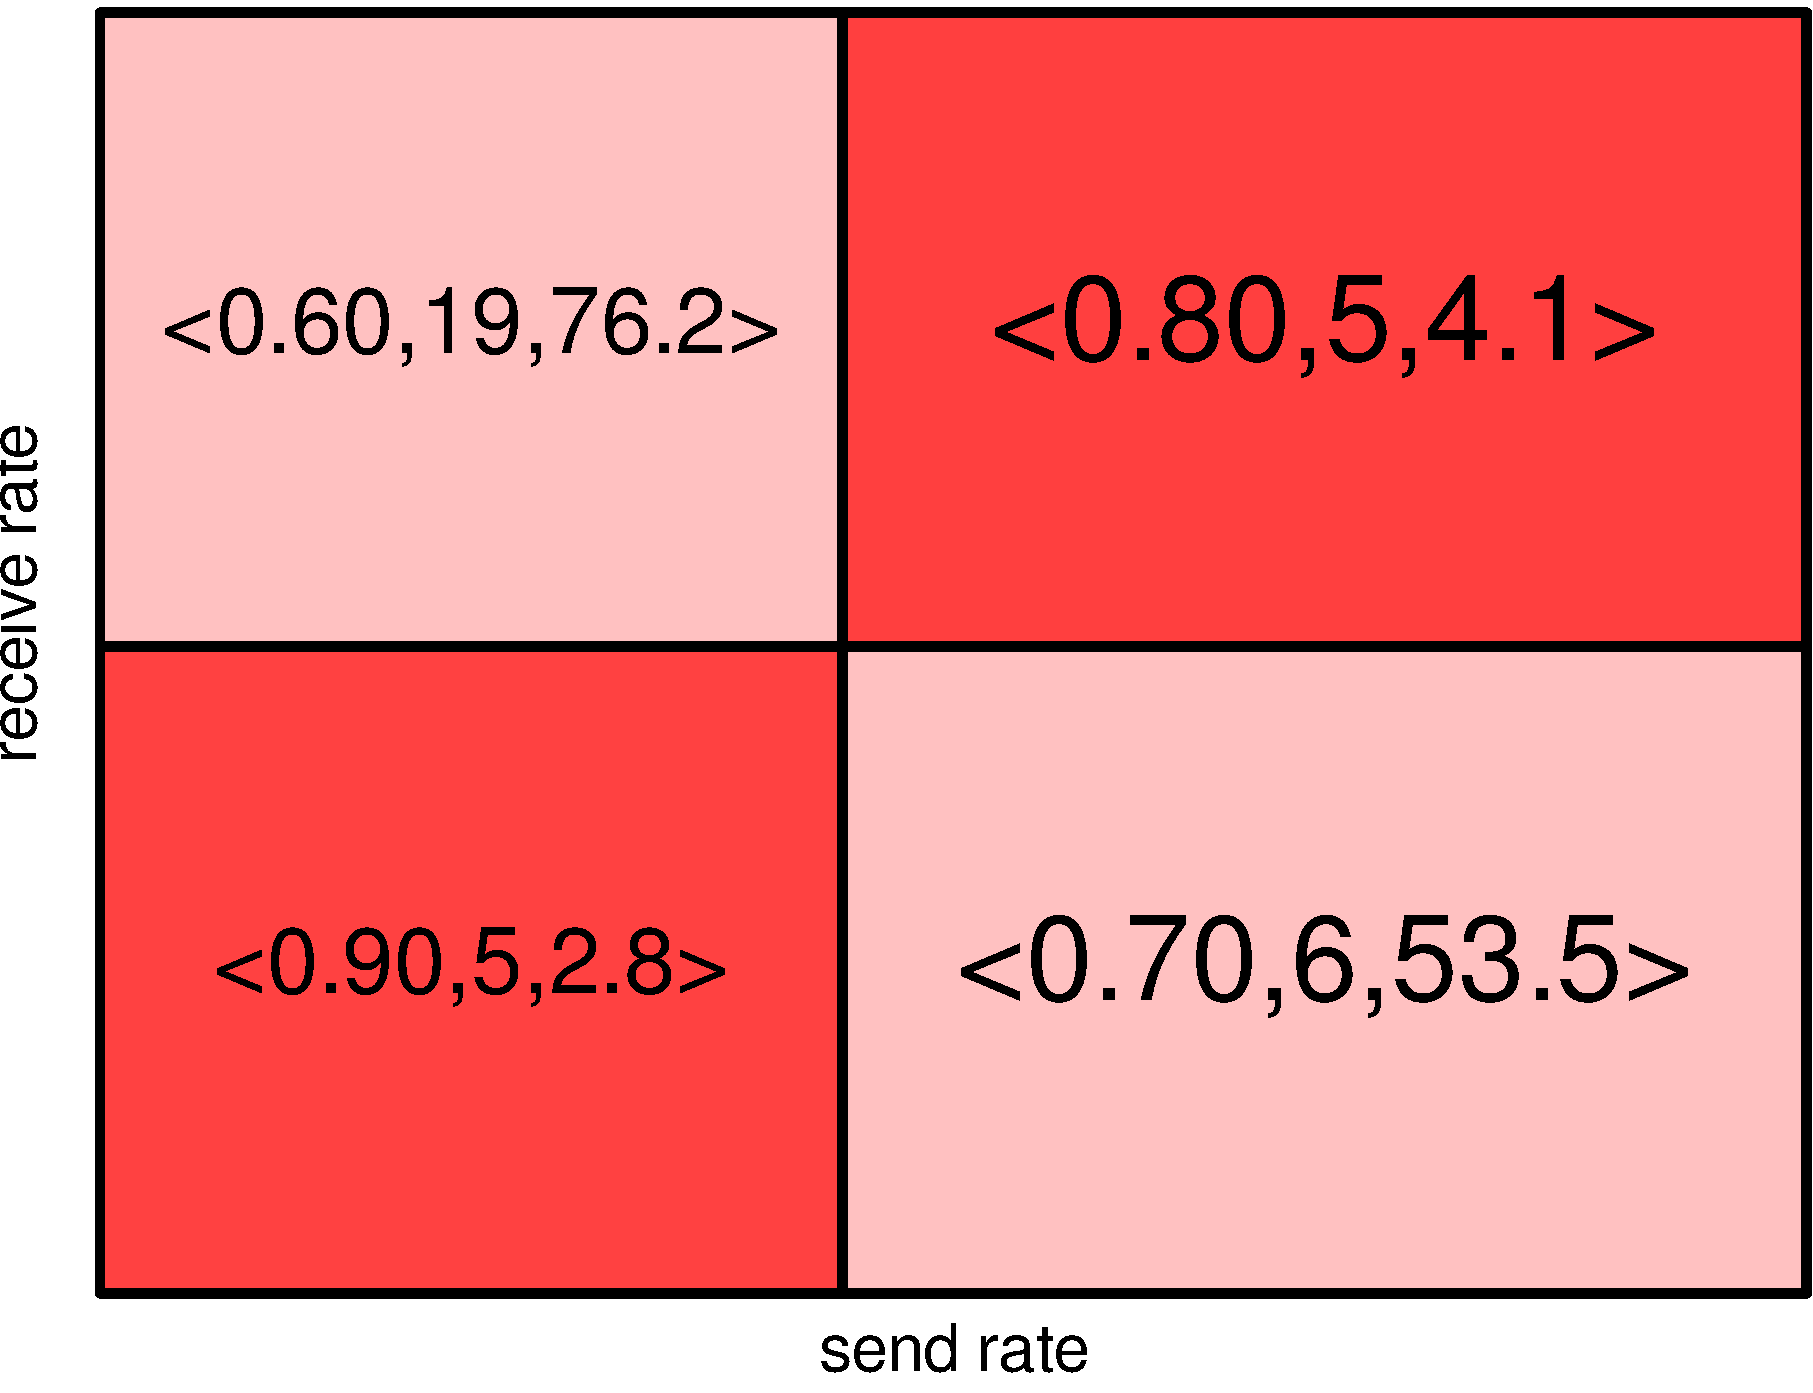
\includegraphics[width=8.5 cm]{remy-graph/graph/test4.pdf}

\end{centering}
\end{frame}

\begin{frame}
\frametitle{Iterate}
\begin{centering}
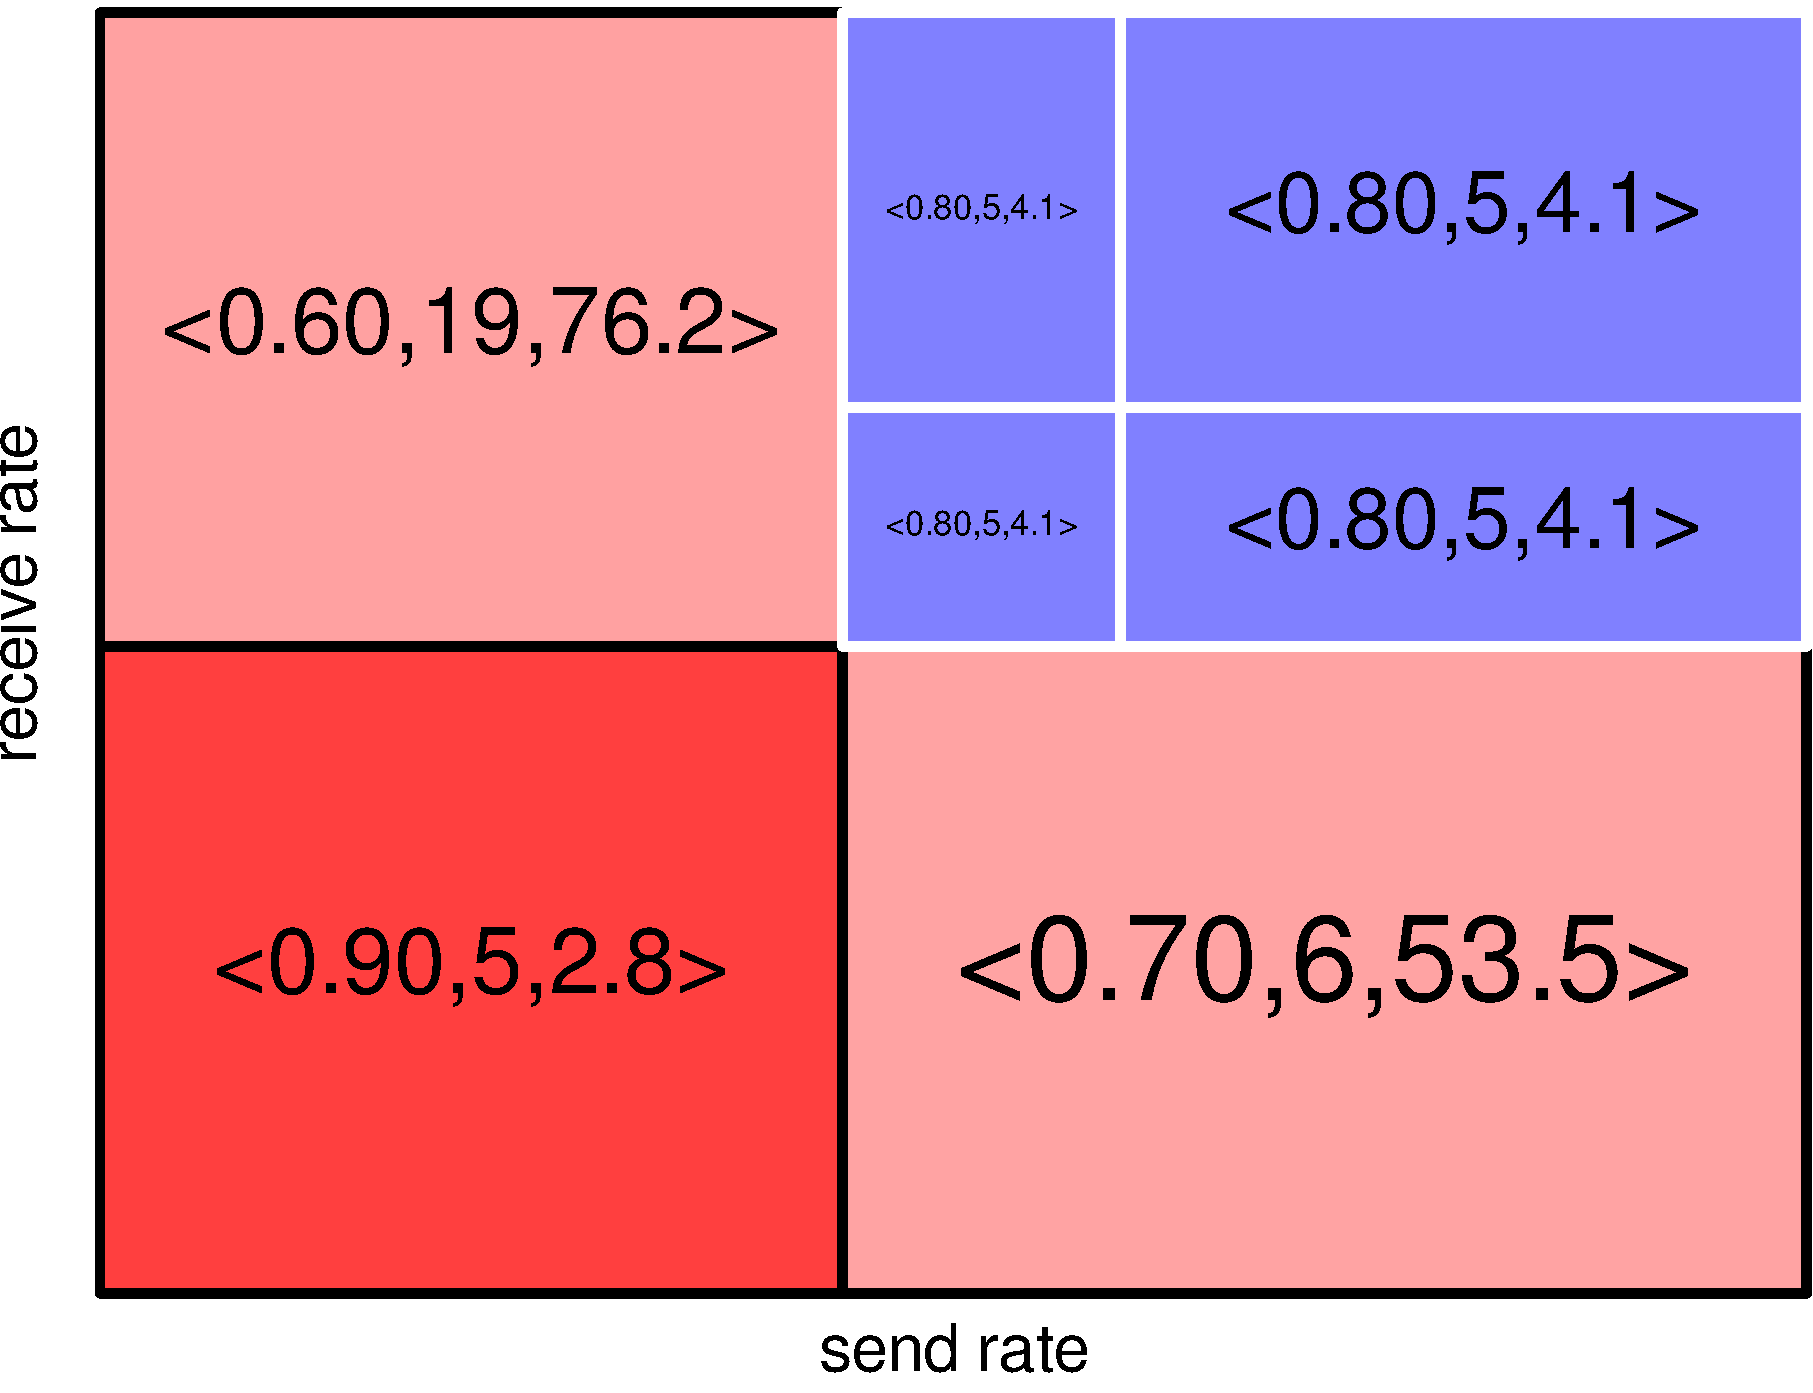
\includegraphics[width=8.5 cm]{remy-graph/graph/test5.pdf}

\end{centering}
\end{frame}

\begin{frame}
\frametitle{Iterate}
\begin{centering}
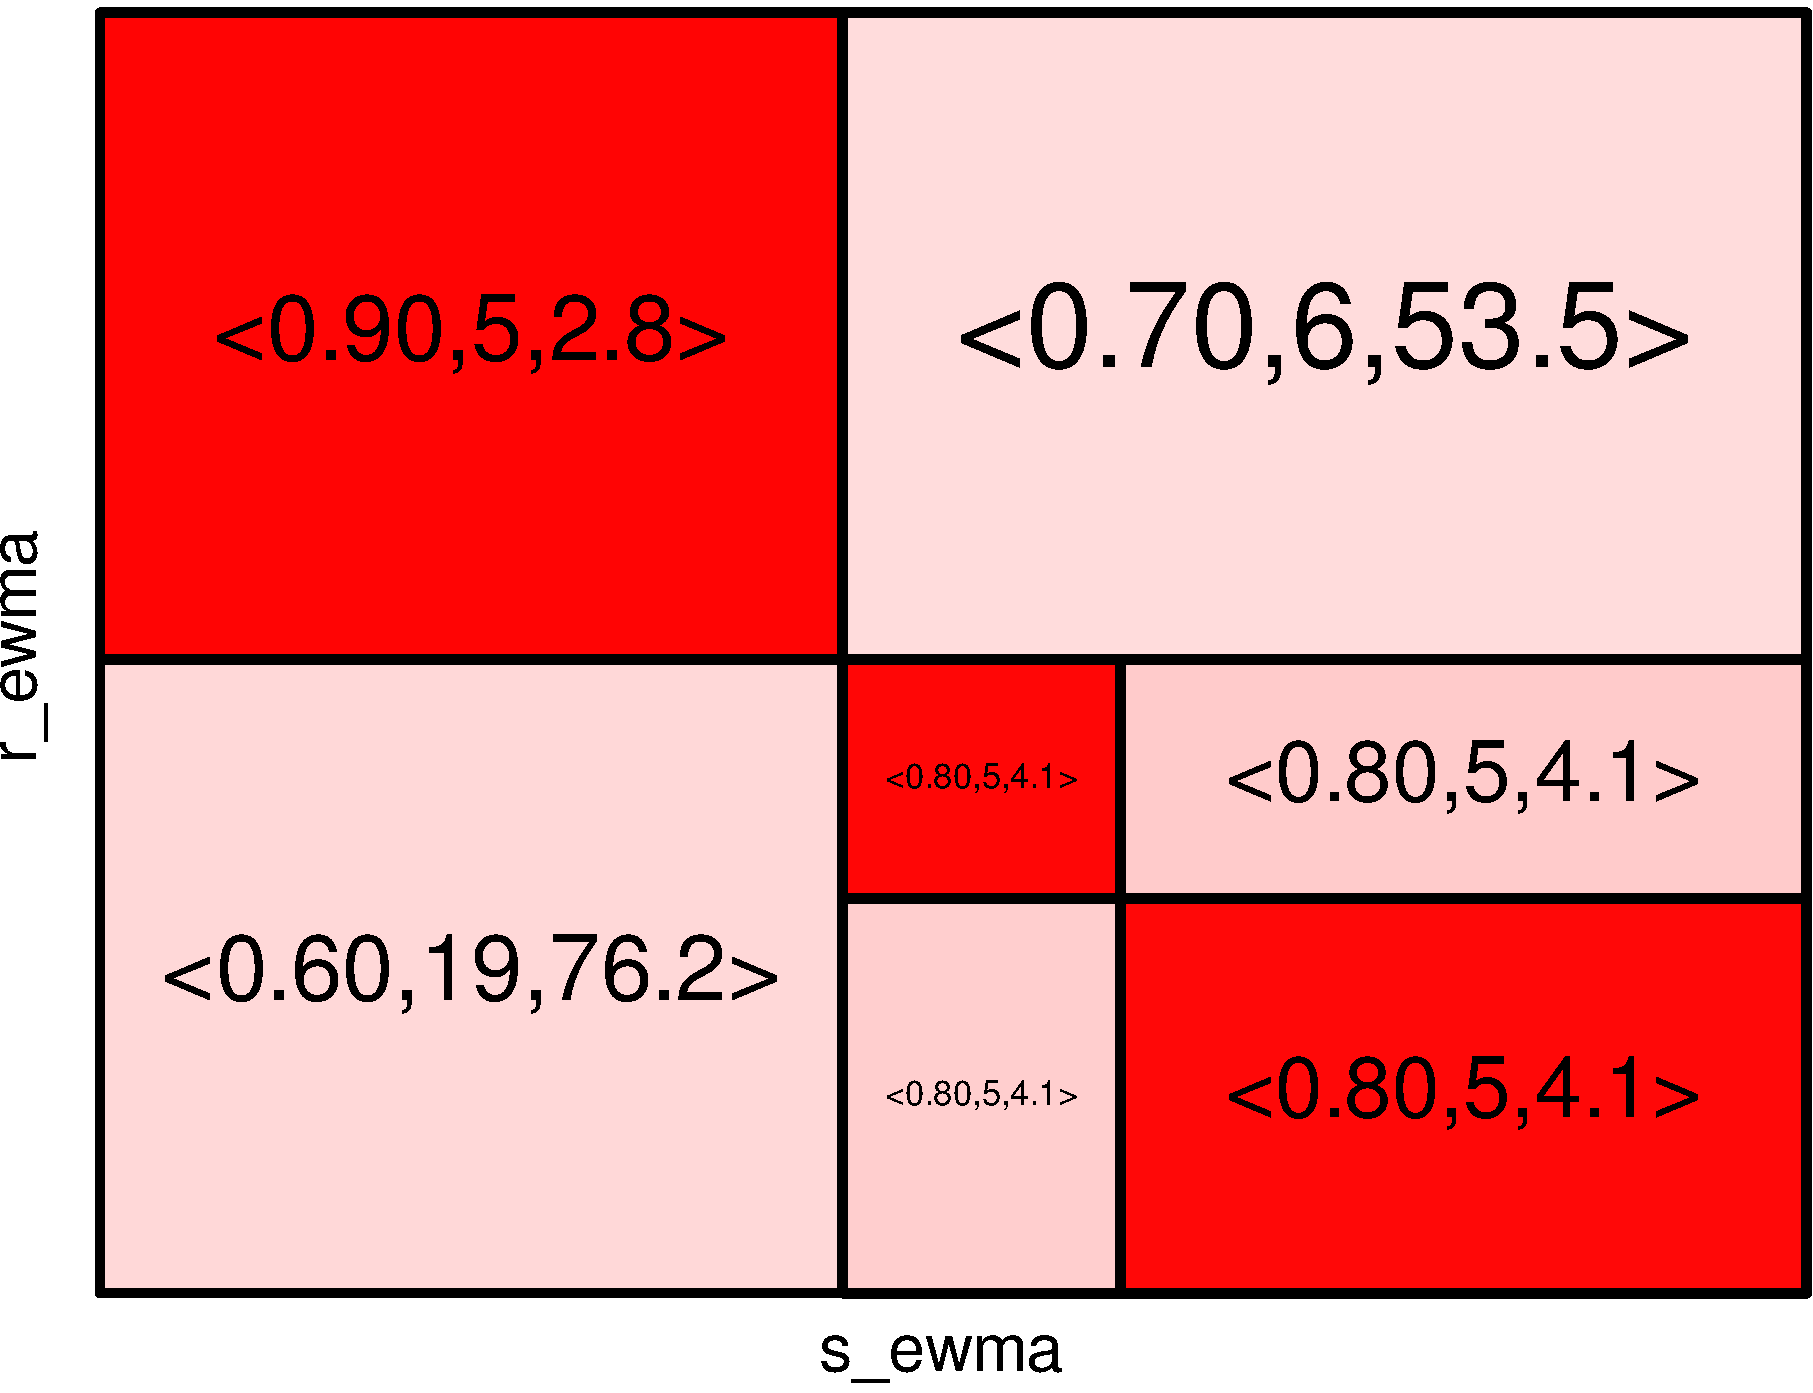
\includegraphics[width=8.5 cm]{remy-graph/graph/test6.pdf}

\end{centering}
\end{frame}
\begin{frame}
\frametitle{Iterate}\begin{centering}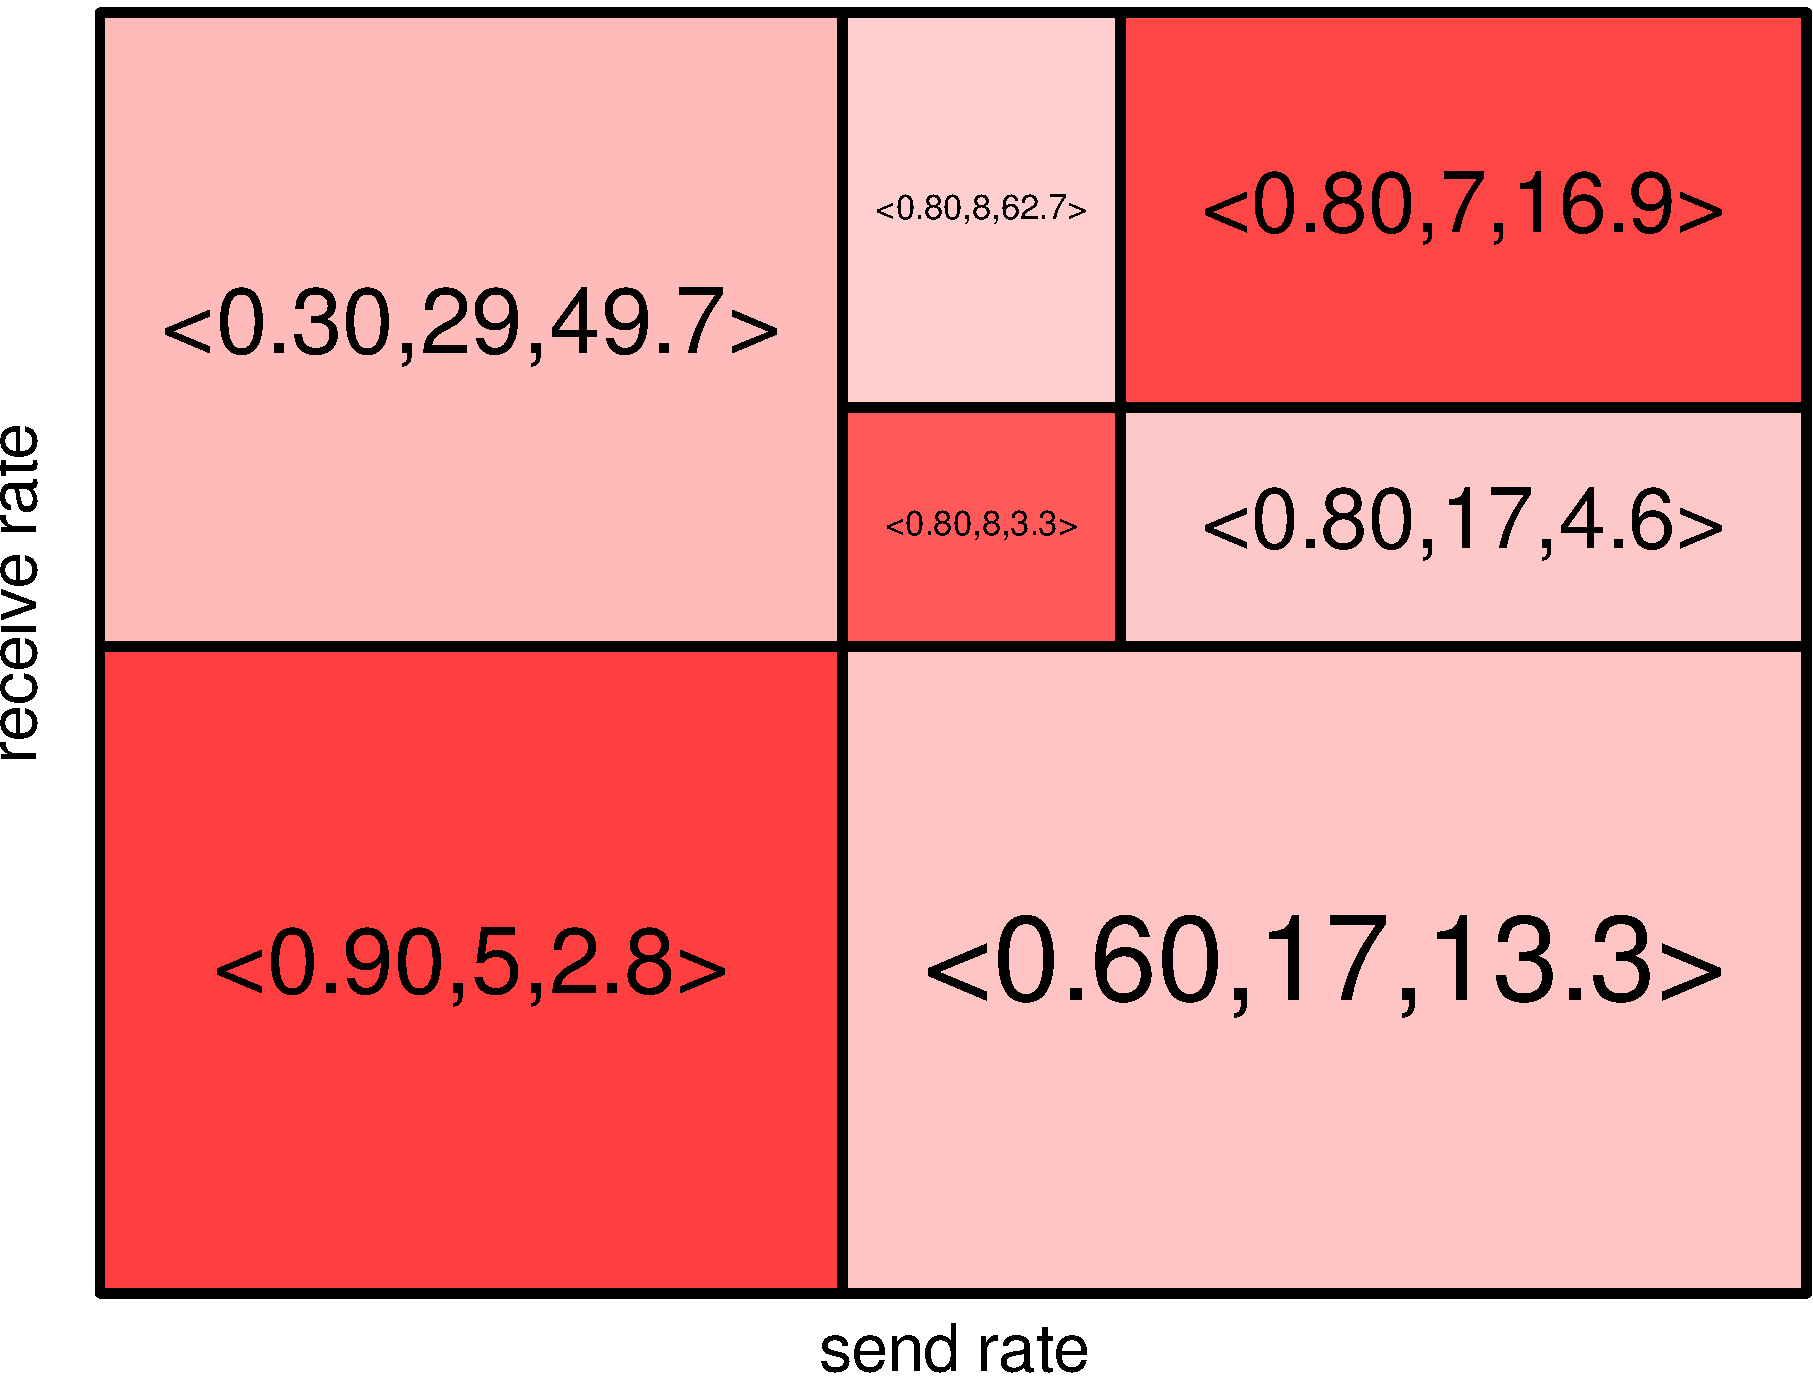
\includegraphics[width=8.5 cm]{remy-graph/graph/test7.pdf}

\end{centering}\end{frame}


\begin{frame}
\frametitle{Iterate}\begin{centering}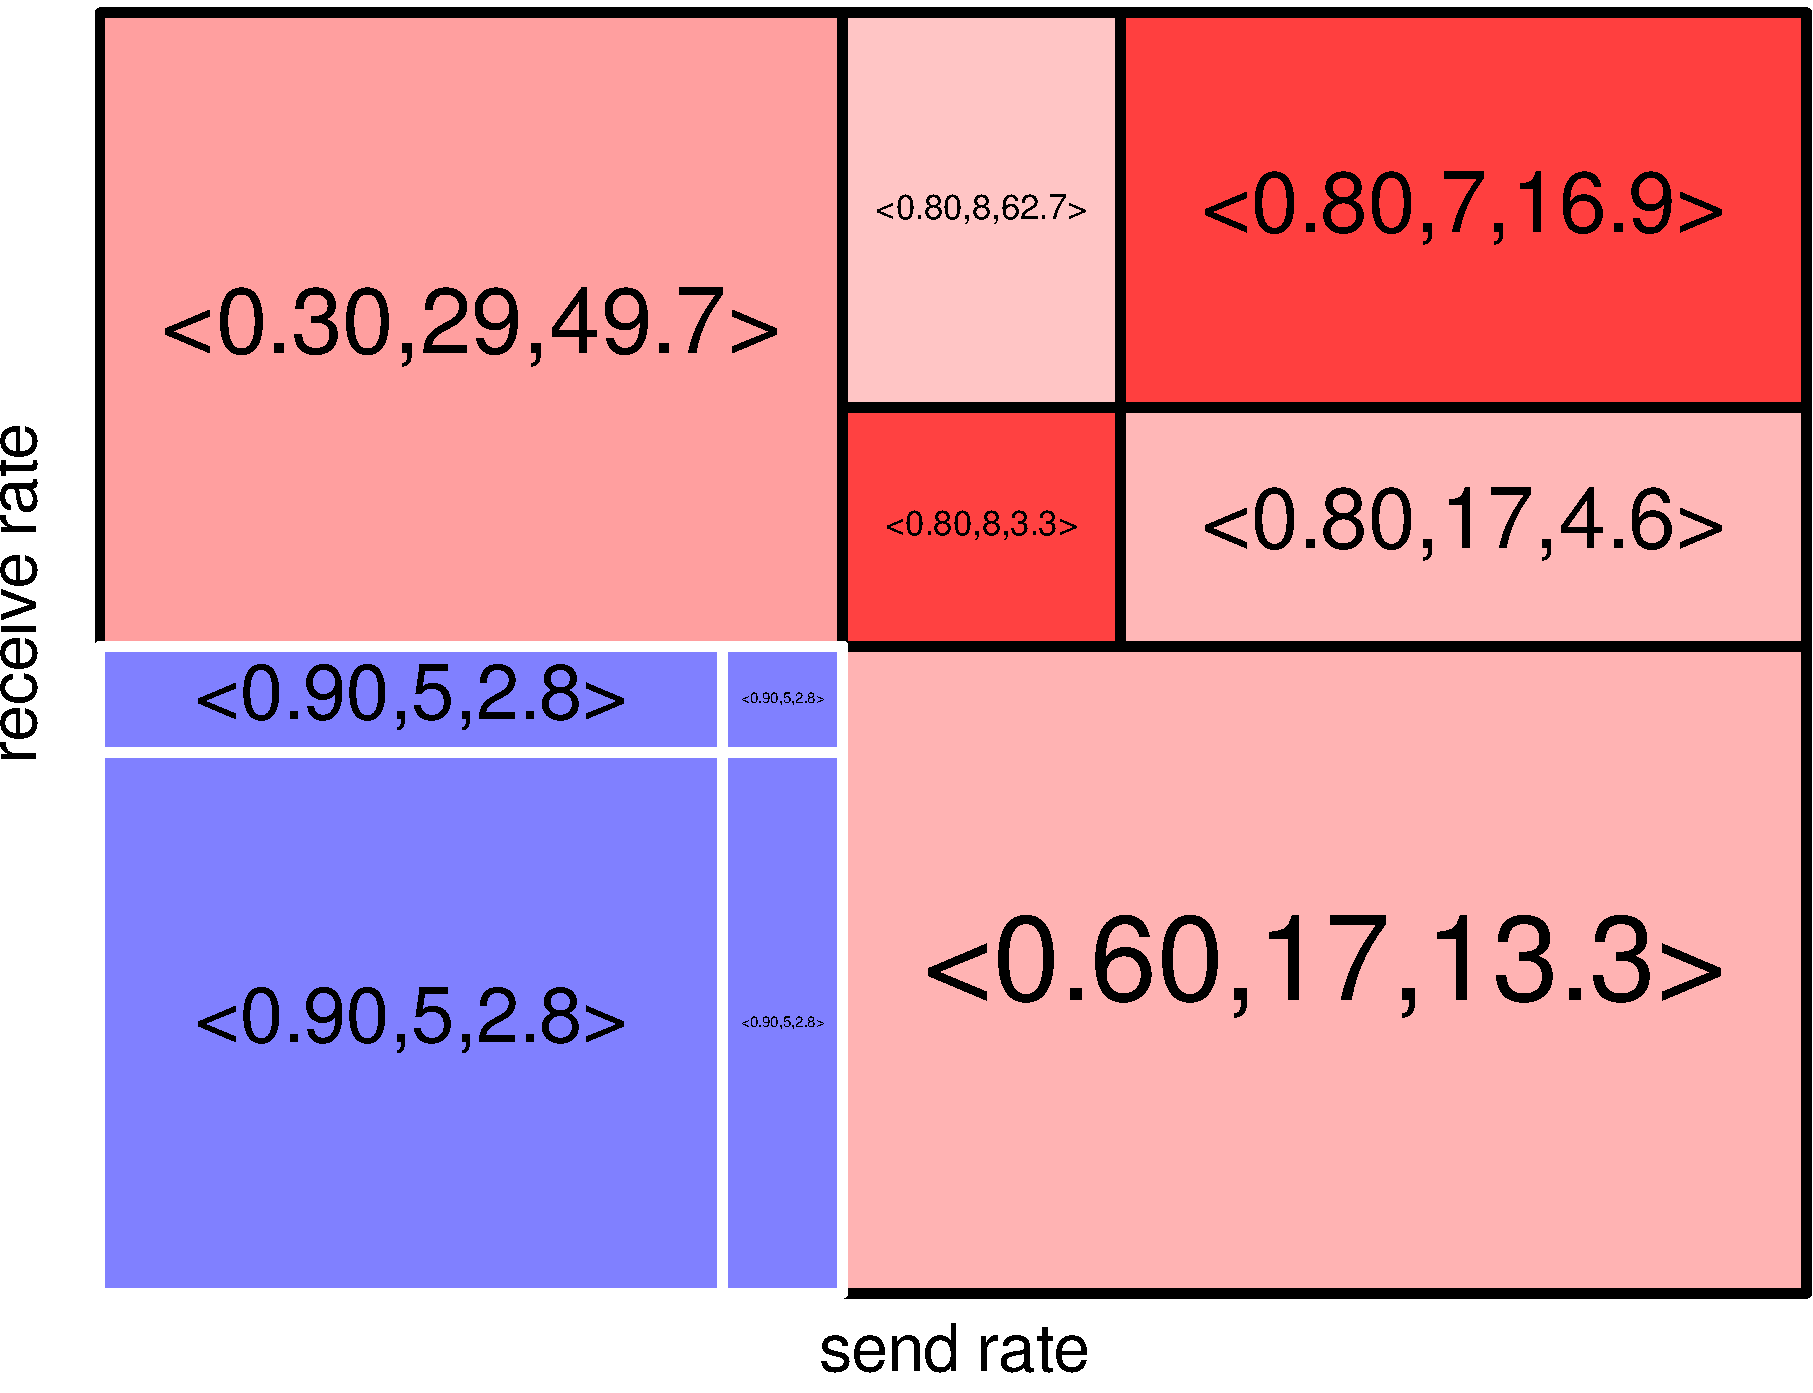
\includegraphics[width=8.5 cm]{remy-graph/graph/test8.pdf}

\end{centering}\end{frame}


\begin{frame}
\frametitle{Iterate}\begin{centering}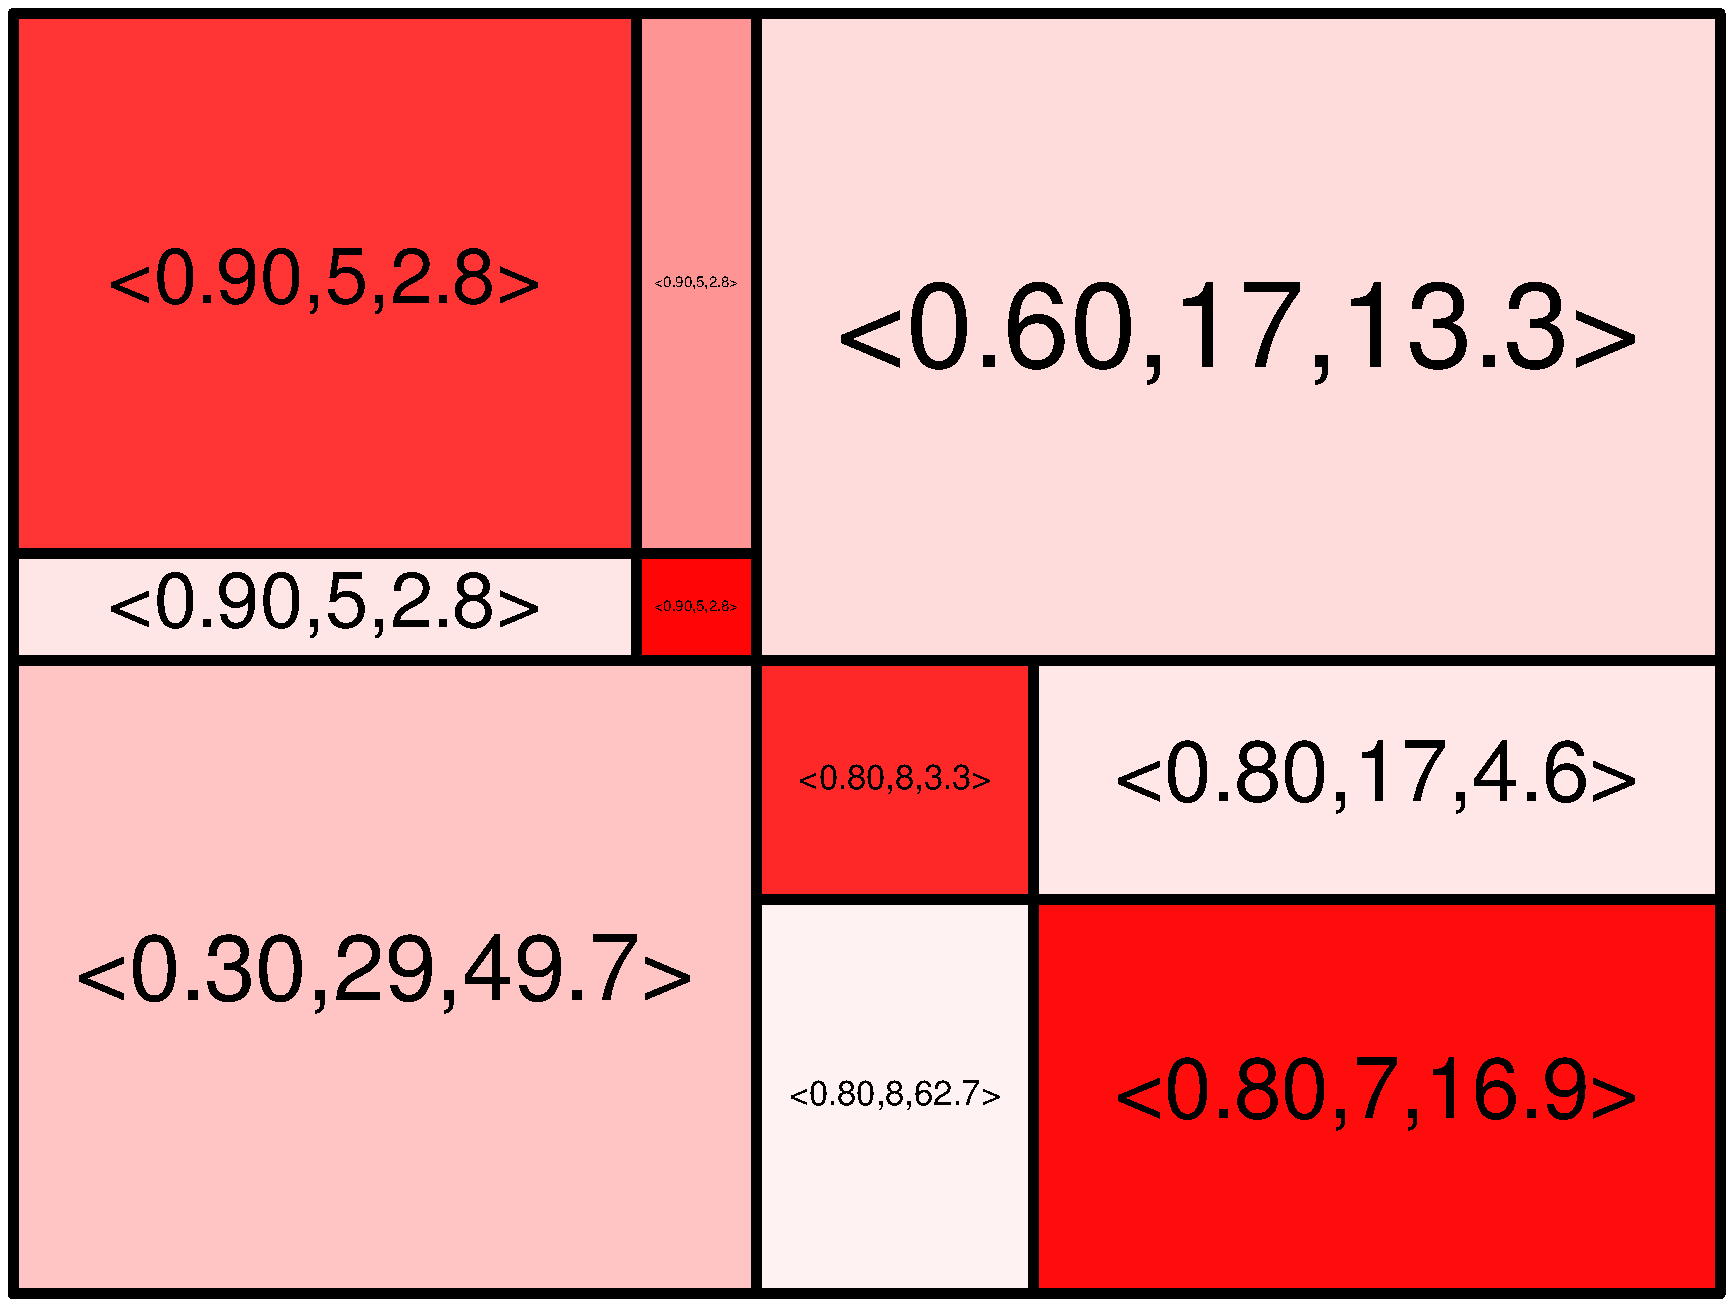
\includegraphics[width=8.5 cm]{remy-graph/graph/test9.pdf}

\end{centering}\end{frame}


\begin{frame}
\frametitle{Iterate}\begin{centering}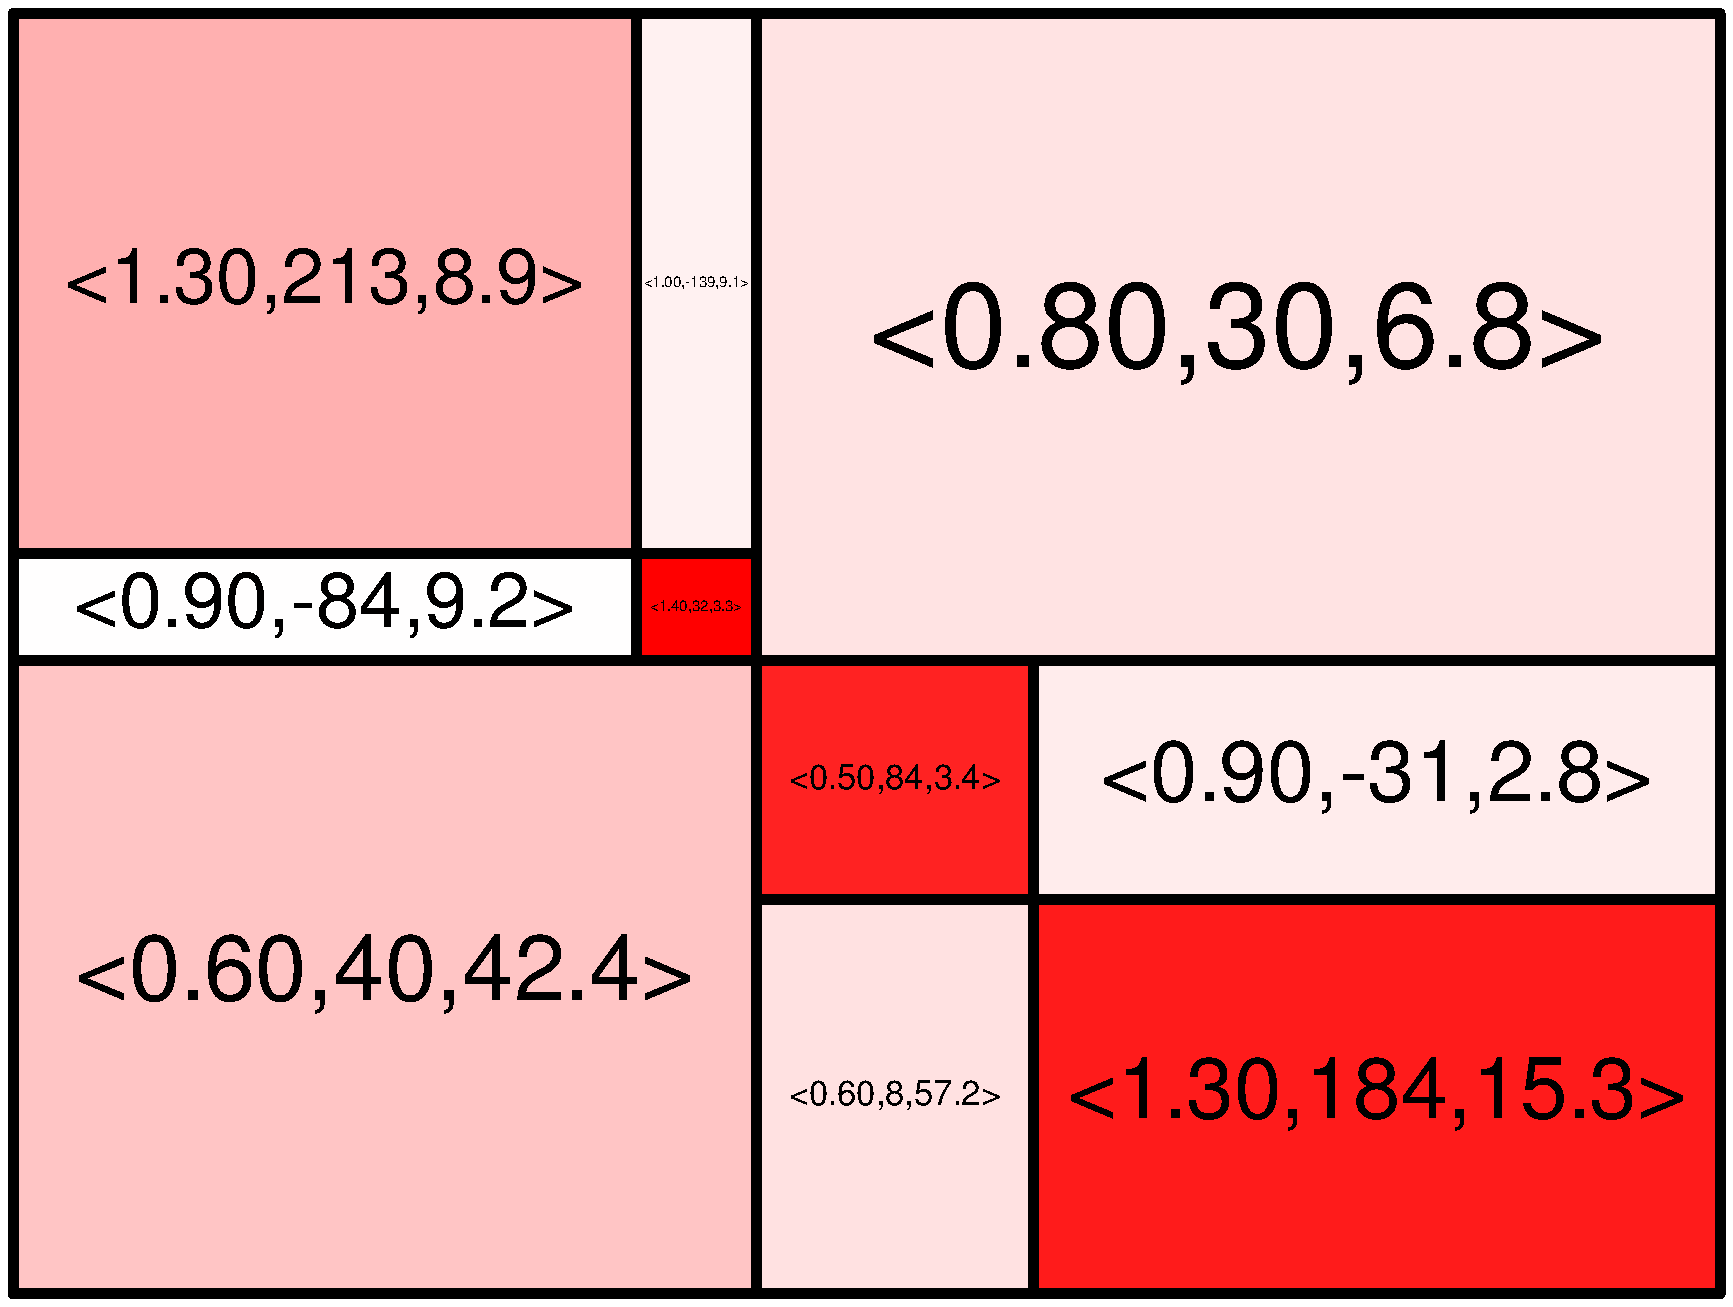
\includegraphics[width=8.5 cm]{remy-graph/graph/test10.pdf}

\end{centering}\end{frame}


\begin{frame}
\frametitle{Iterate}\begin{centering}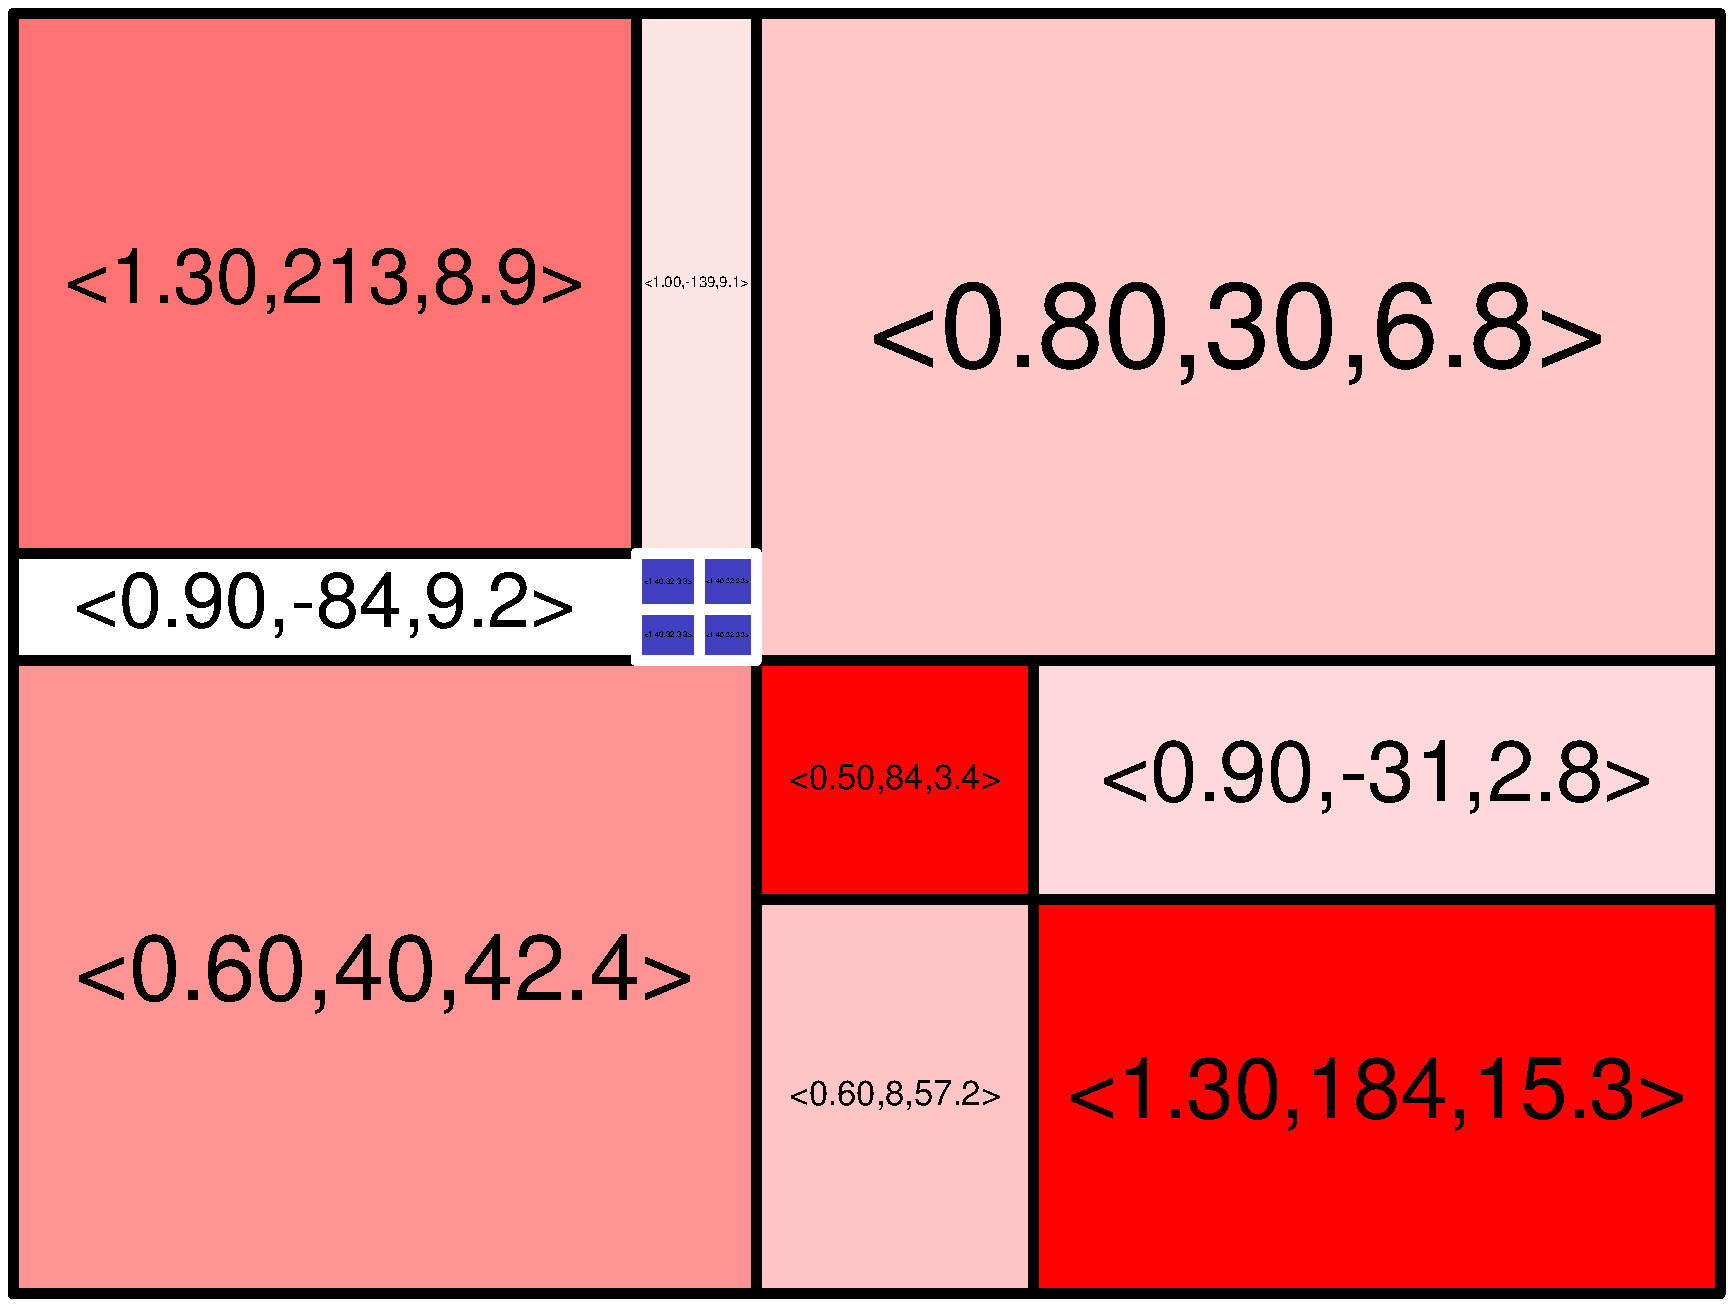
\includegraphics[width=8.5 cm]{remy-graph/graph/test11.pdf}

\end{centering}\end{frame}


\begin{frame}
\frametitle{Iterate}\begin{centering}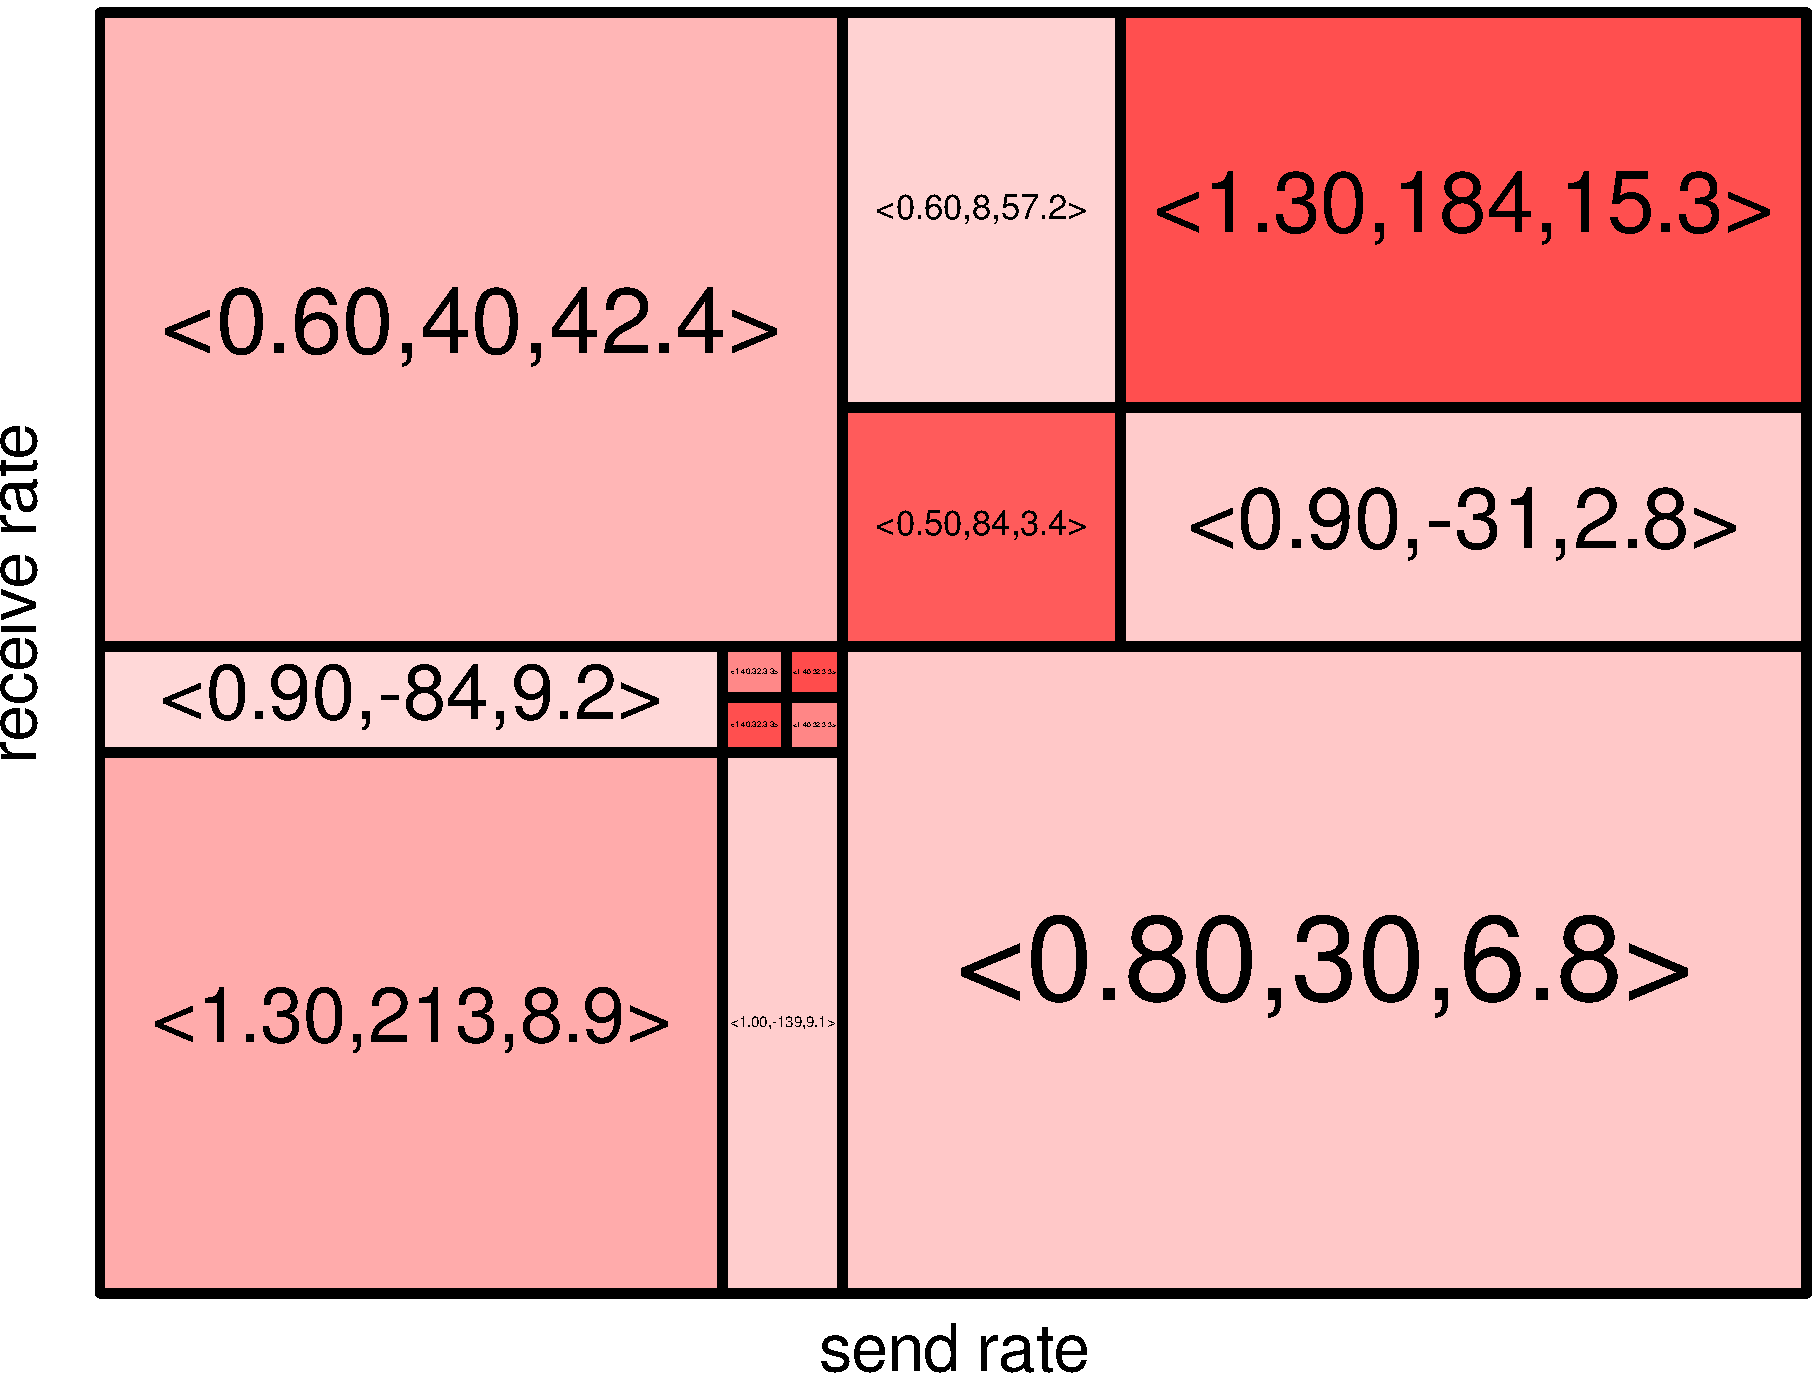
\includegraphics[width=8.5 cm]{remy-graph/graph/test12.pdf}

\end{centering}\end{frame}


\begin{frame}
\frametitle{Iterate}\begin{centering}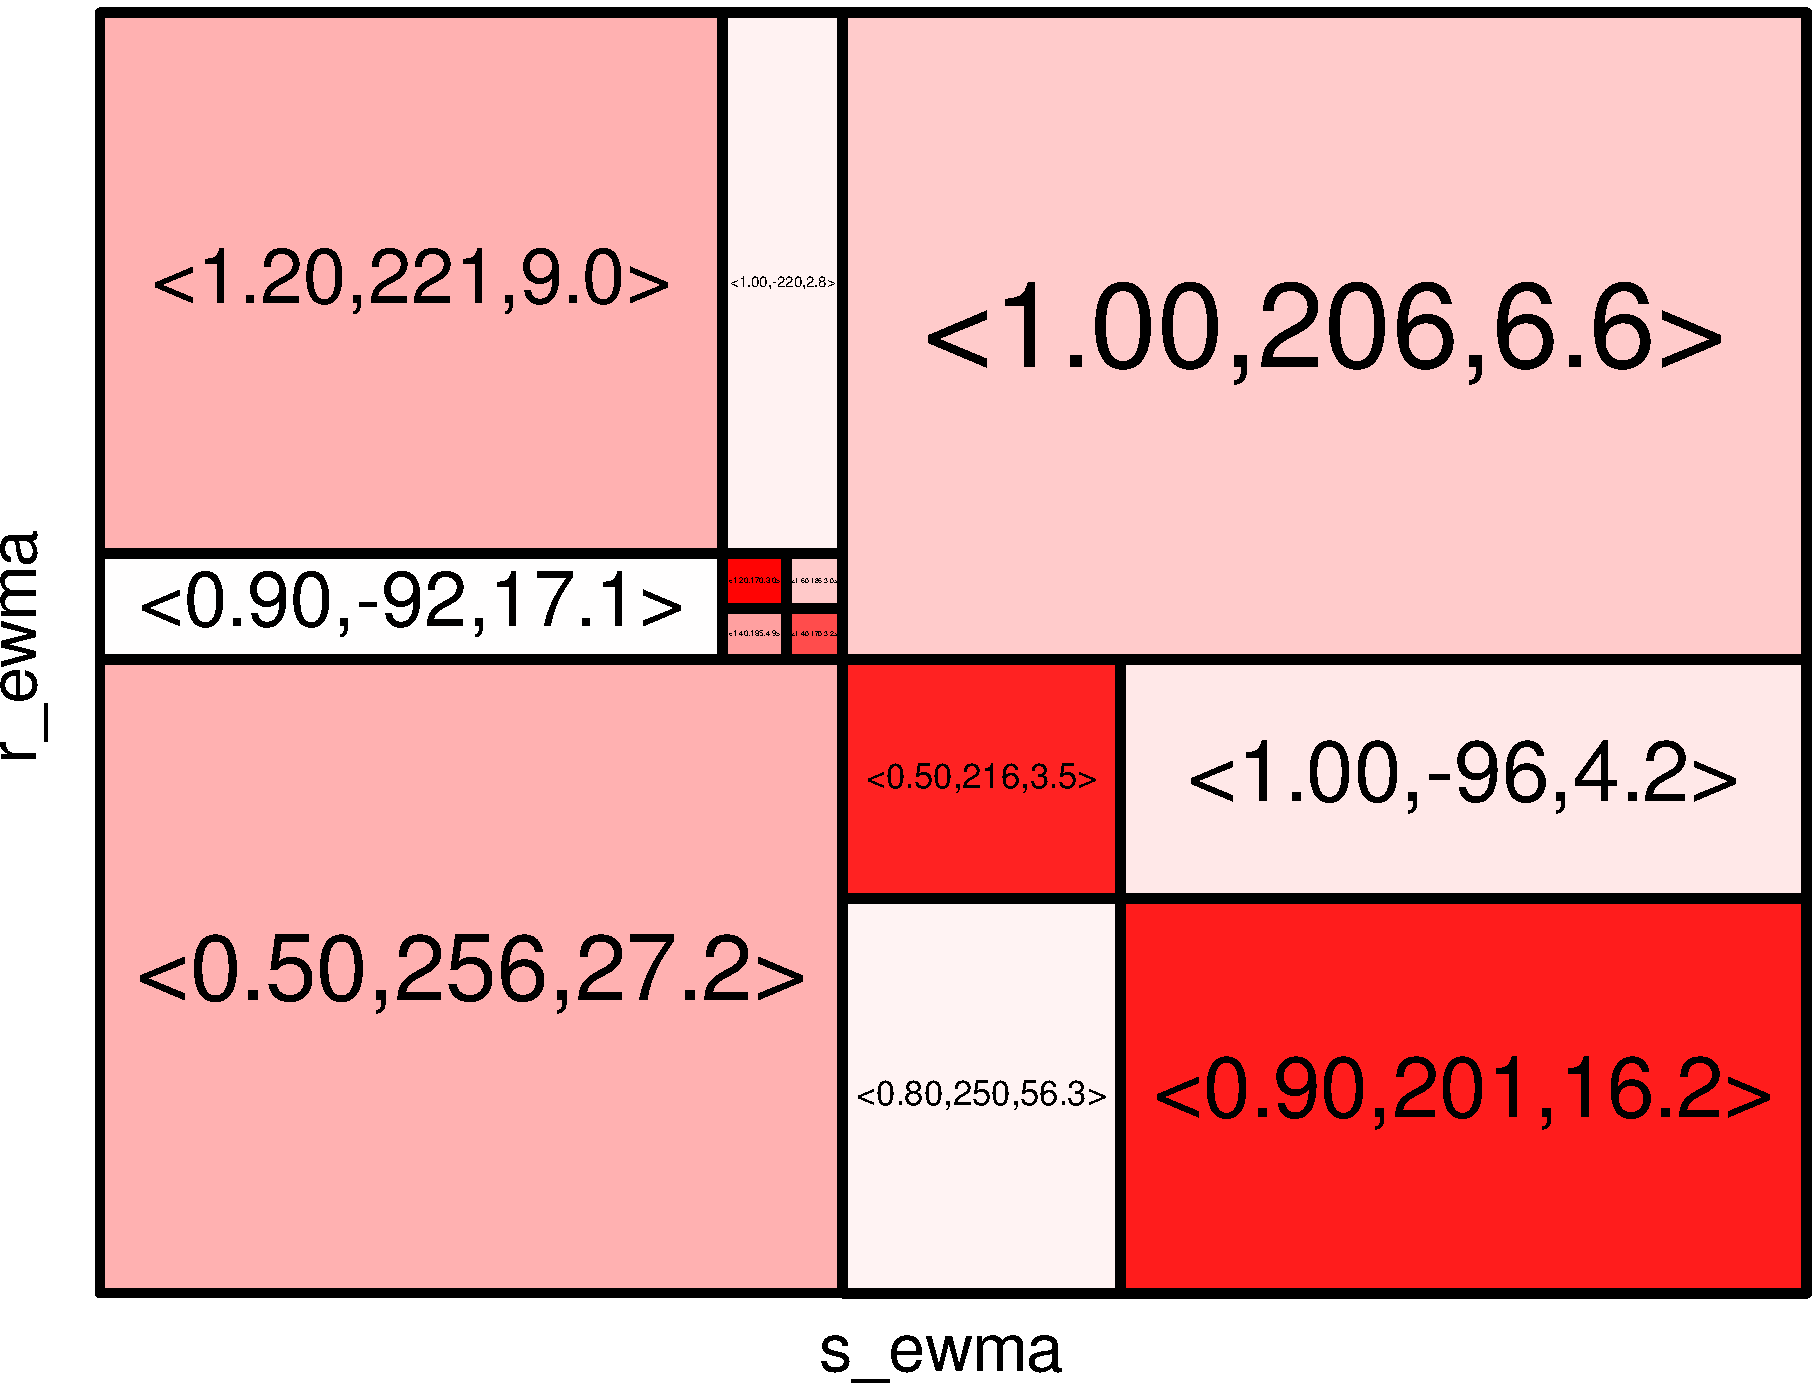
\includegraphics[width=8.5 cm]{remy-graph/graph/test13.pdf}

\end{centering}\end{frame}


\begin{frame}
\frametitle{Iterate}\begin{centering}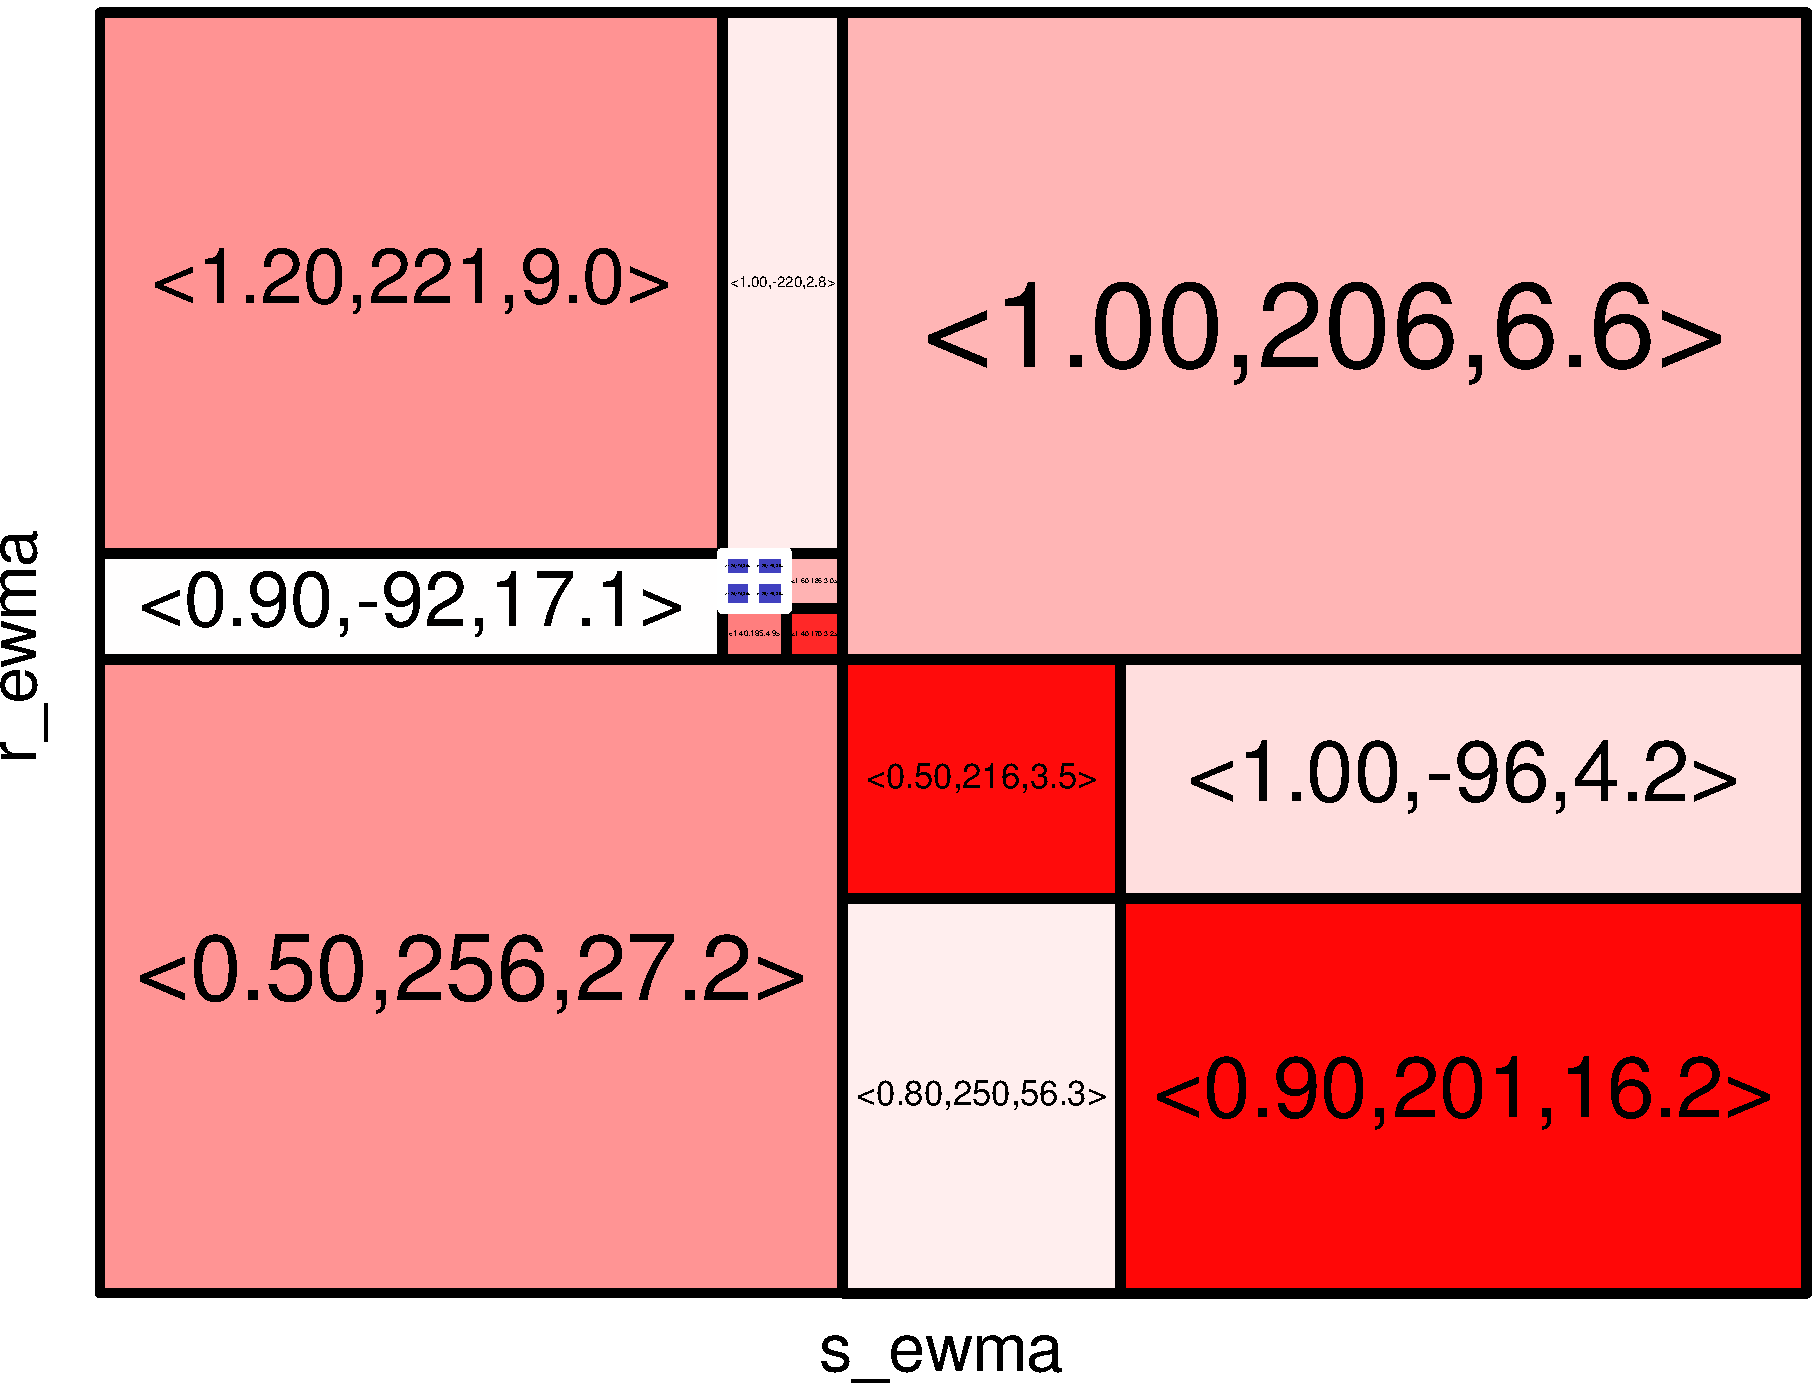
\includegraphics[width=8.5 cm]{remy-graph/graph/test14.pdf}

\end{centering}\end{frame}


\begin{frame}
\frametitle{Iterate}\begin{centering}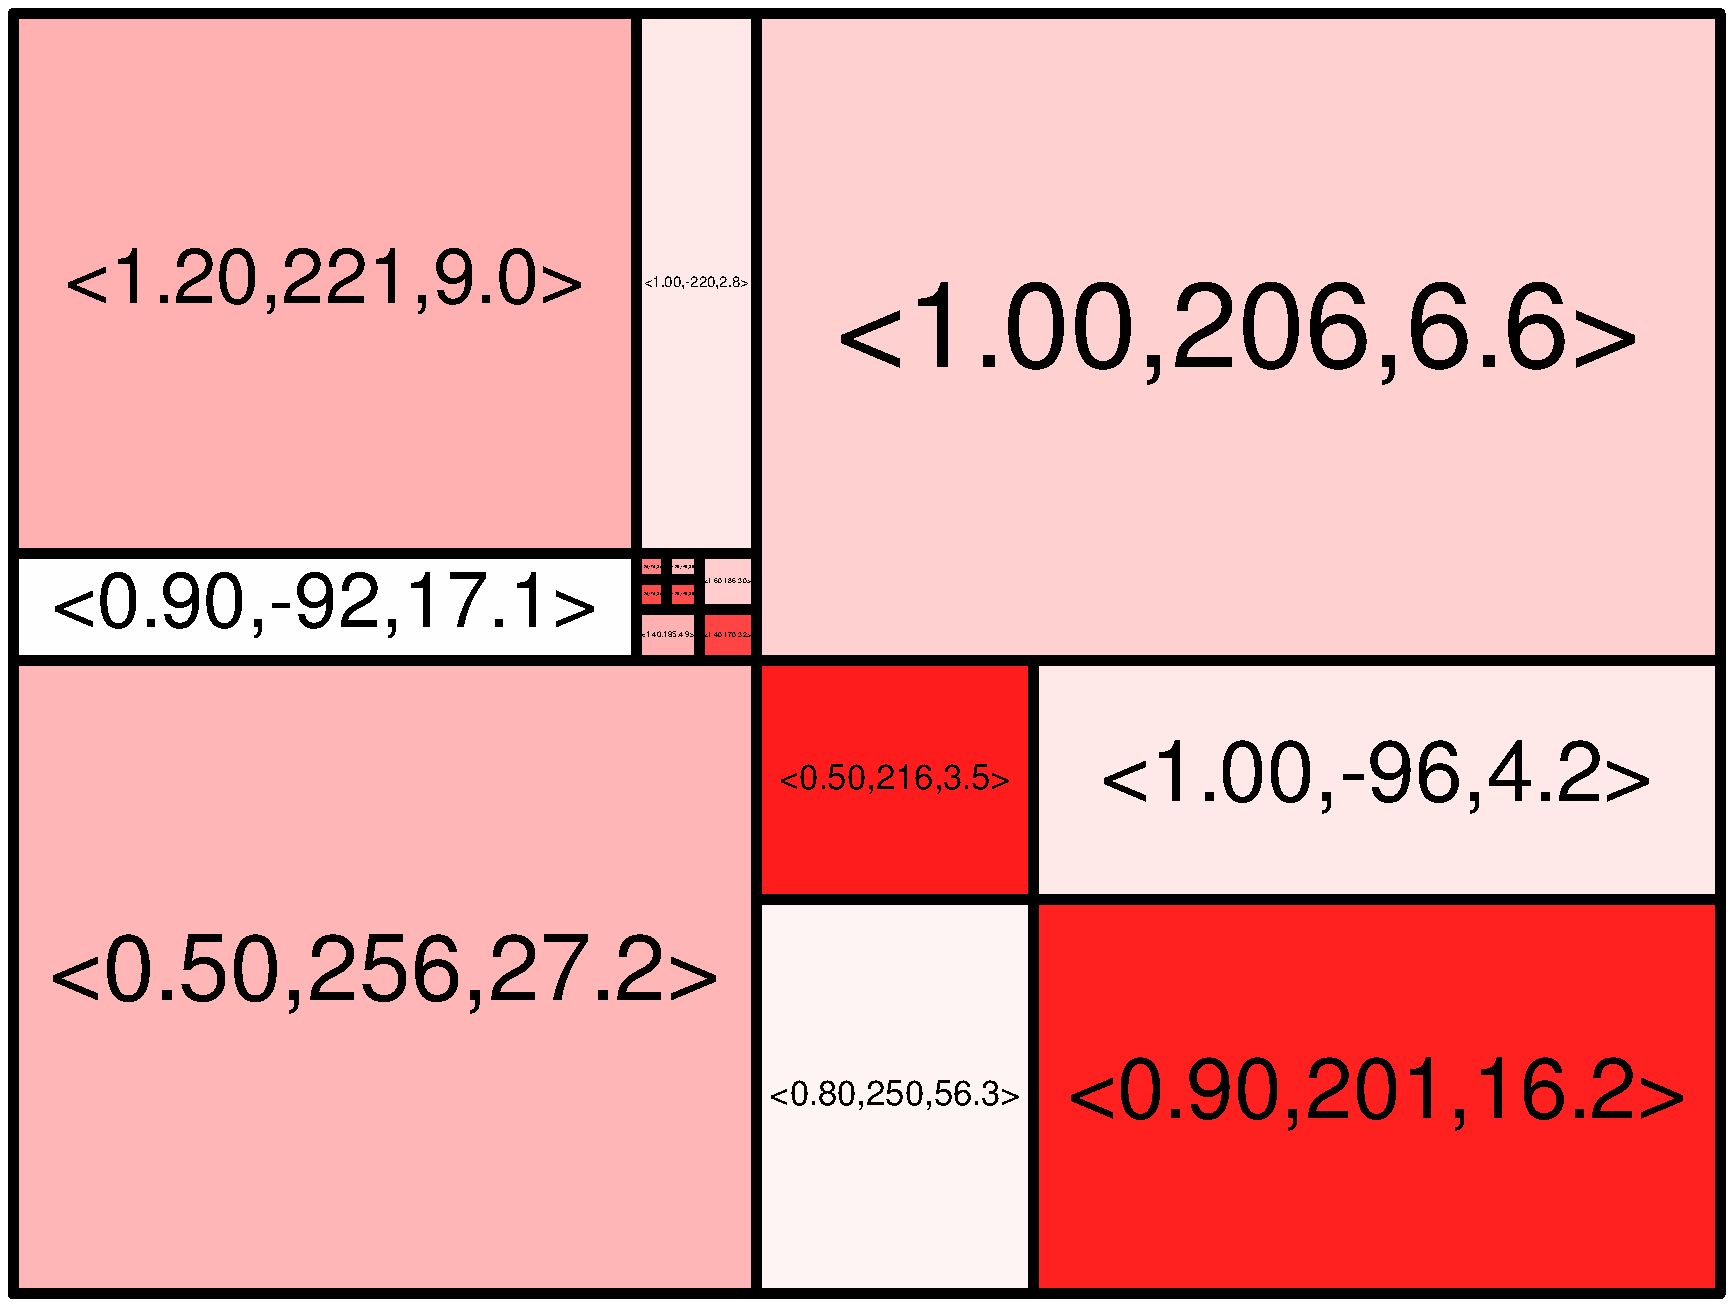
\includegraphics[width=8.5 cm]{remy-graph/graph/test15.pdf}

\end{centering}\end{frame}


\begin{frame}
\frametitle{Iterate}\begin{centering}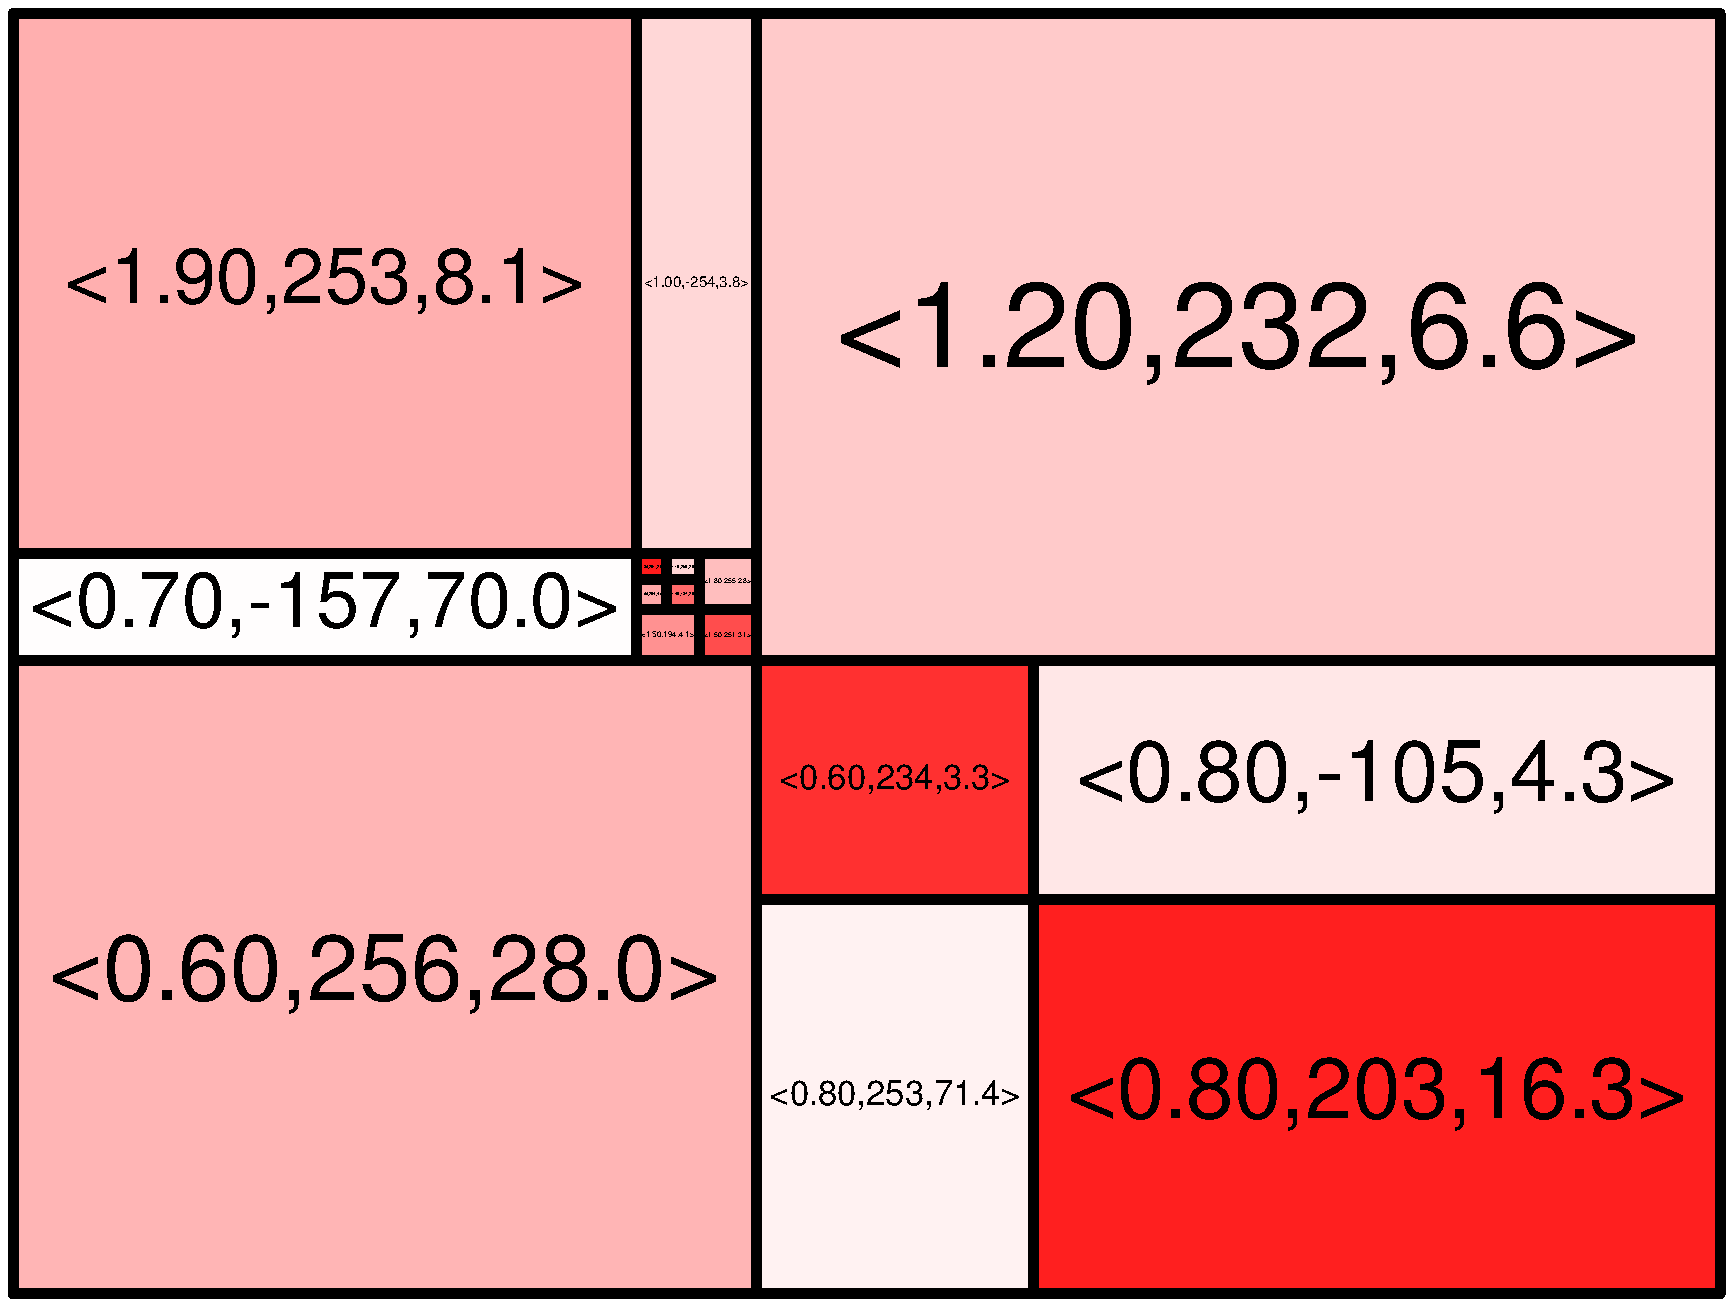
\includegraphics[width=8.5 cm]{remy-graph/graph/test16.pdf}

\end{centering}\end{frame}


\begin{frame}
\frametitle{Iterate}\begin{centering}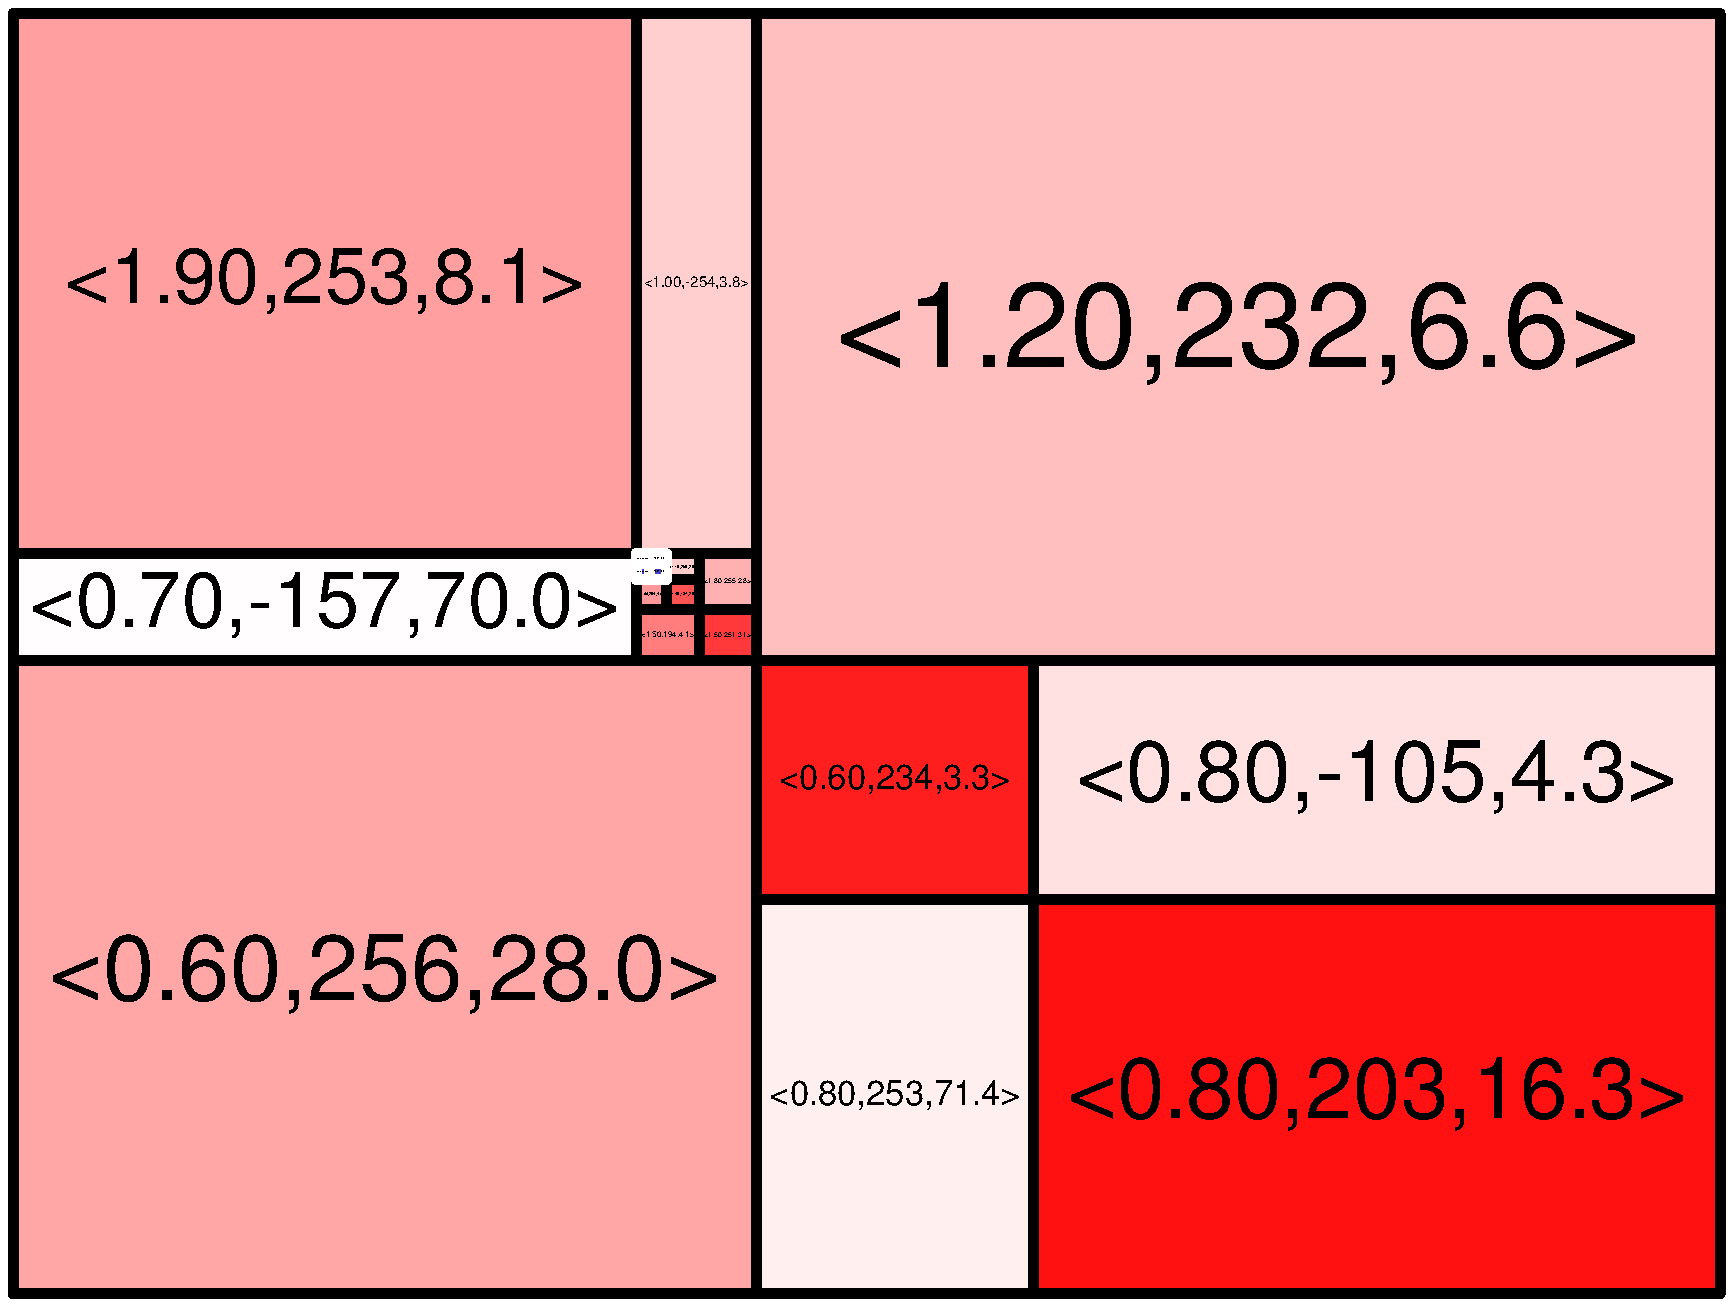
\includegraphics[width=8.5 cm]{remy-graph/graph/test17.pdf}

\end{centering}\end{frame}


\begin{frame}
\frametitle{Iterate}\begin{centering}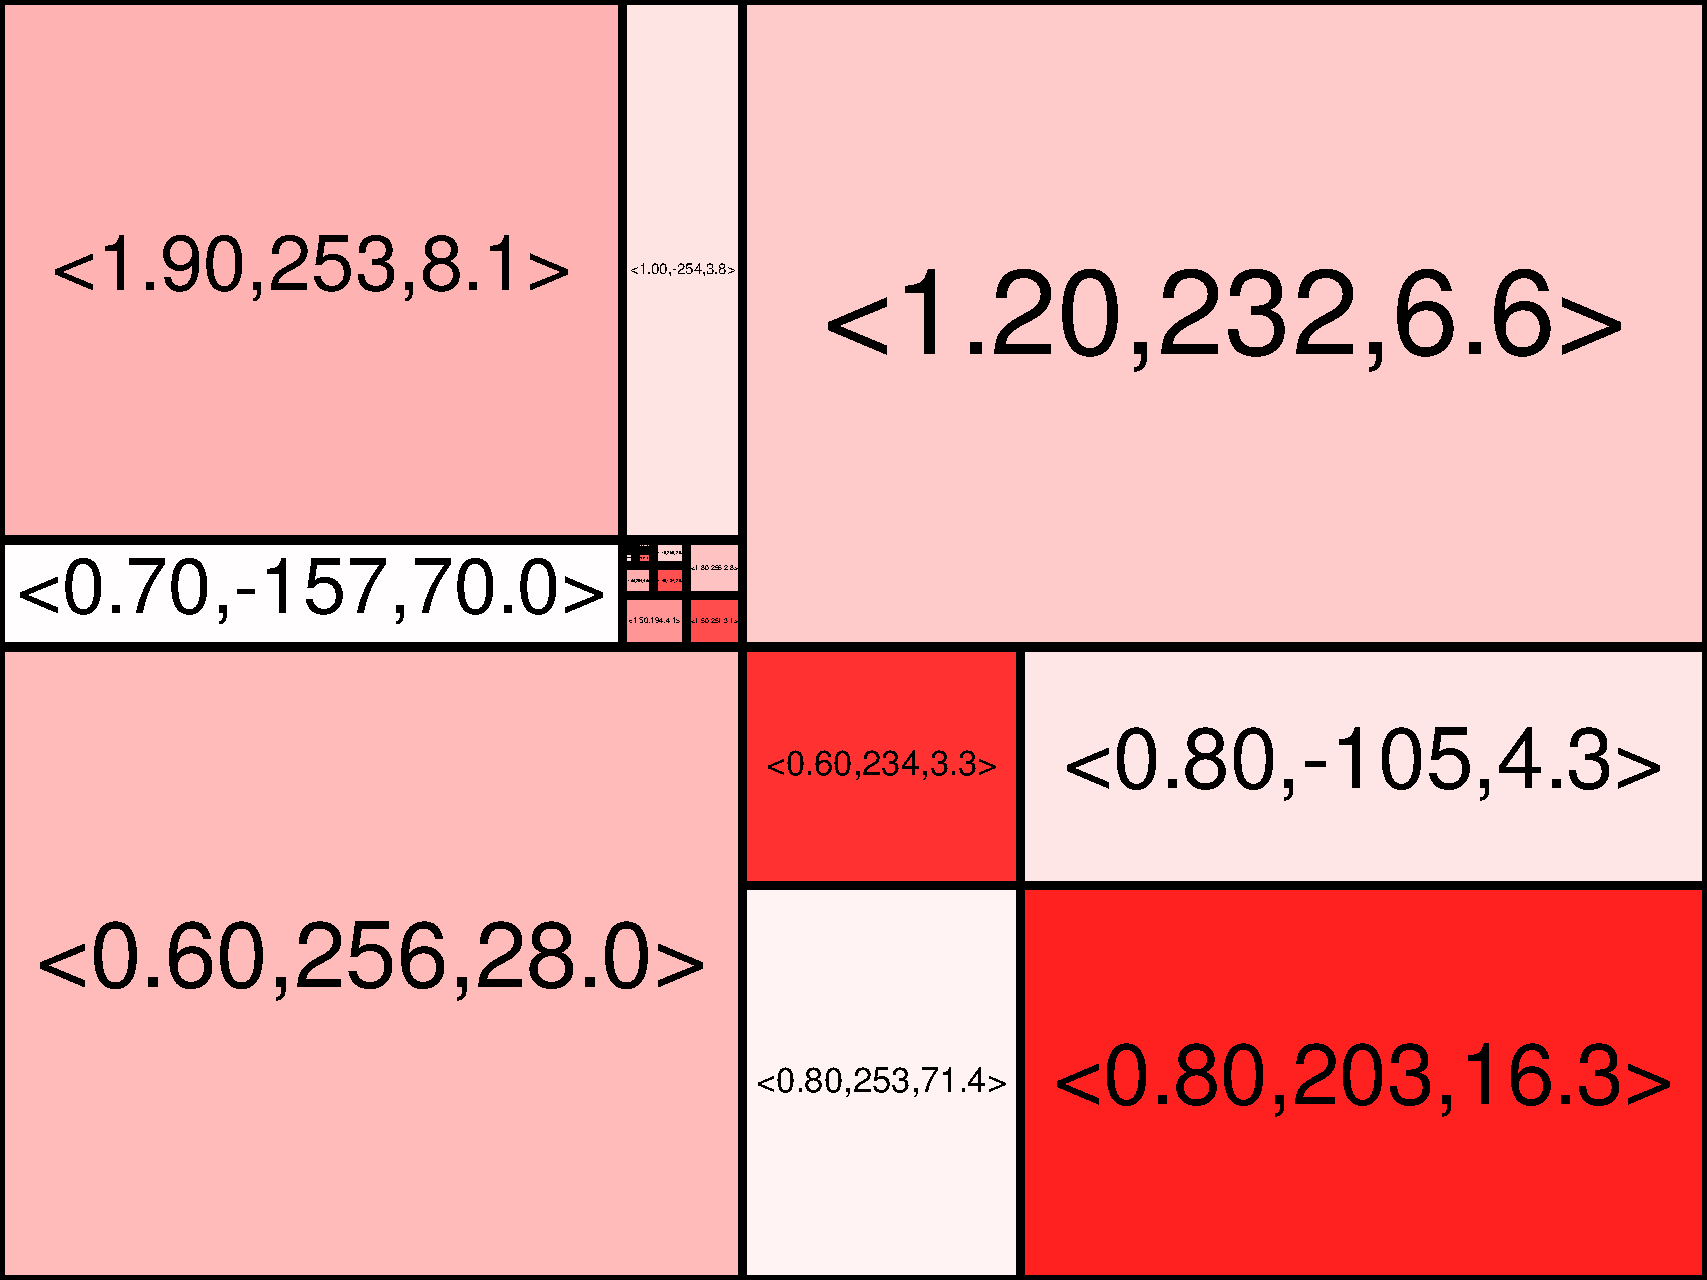
\includegraphics[width=8.5 cm]{remy-graph/graph/test18.pdf}

\end{centering}\end{frame}


\begin{frame}
\frametitle{Iterate}\begin{centering}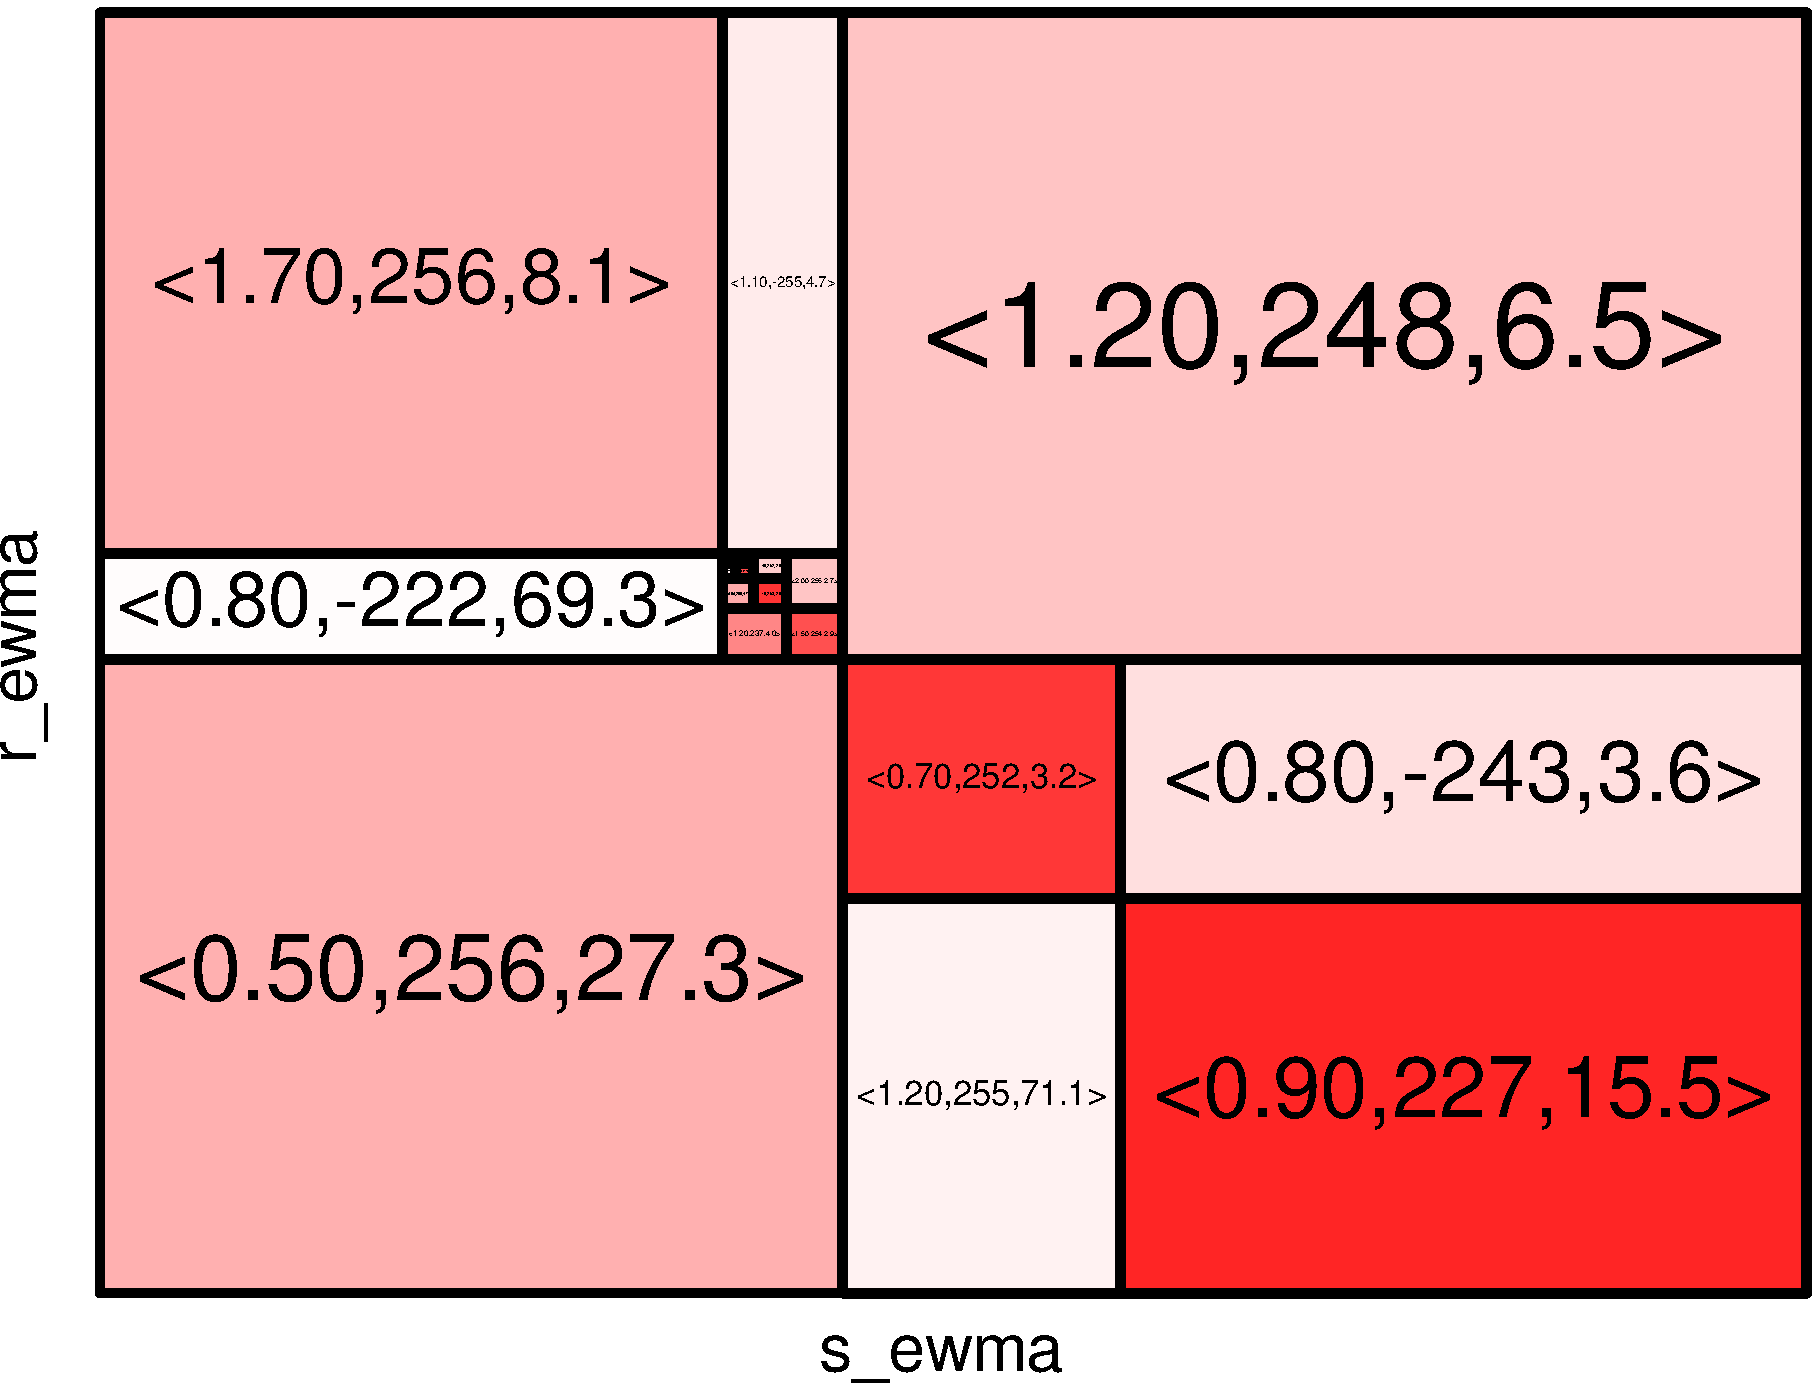
\includegraphics[width=8.5 cm]{remy-graph/graph/test19.pdf}

\end{centering}\end{frame}


\begin{frame}
\frametitle{Iterate}\begin{centering}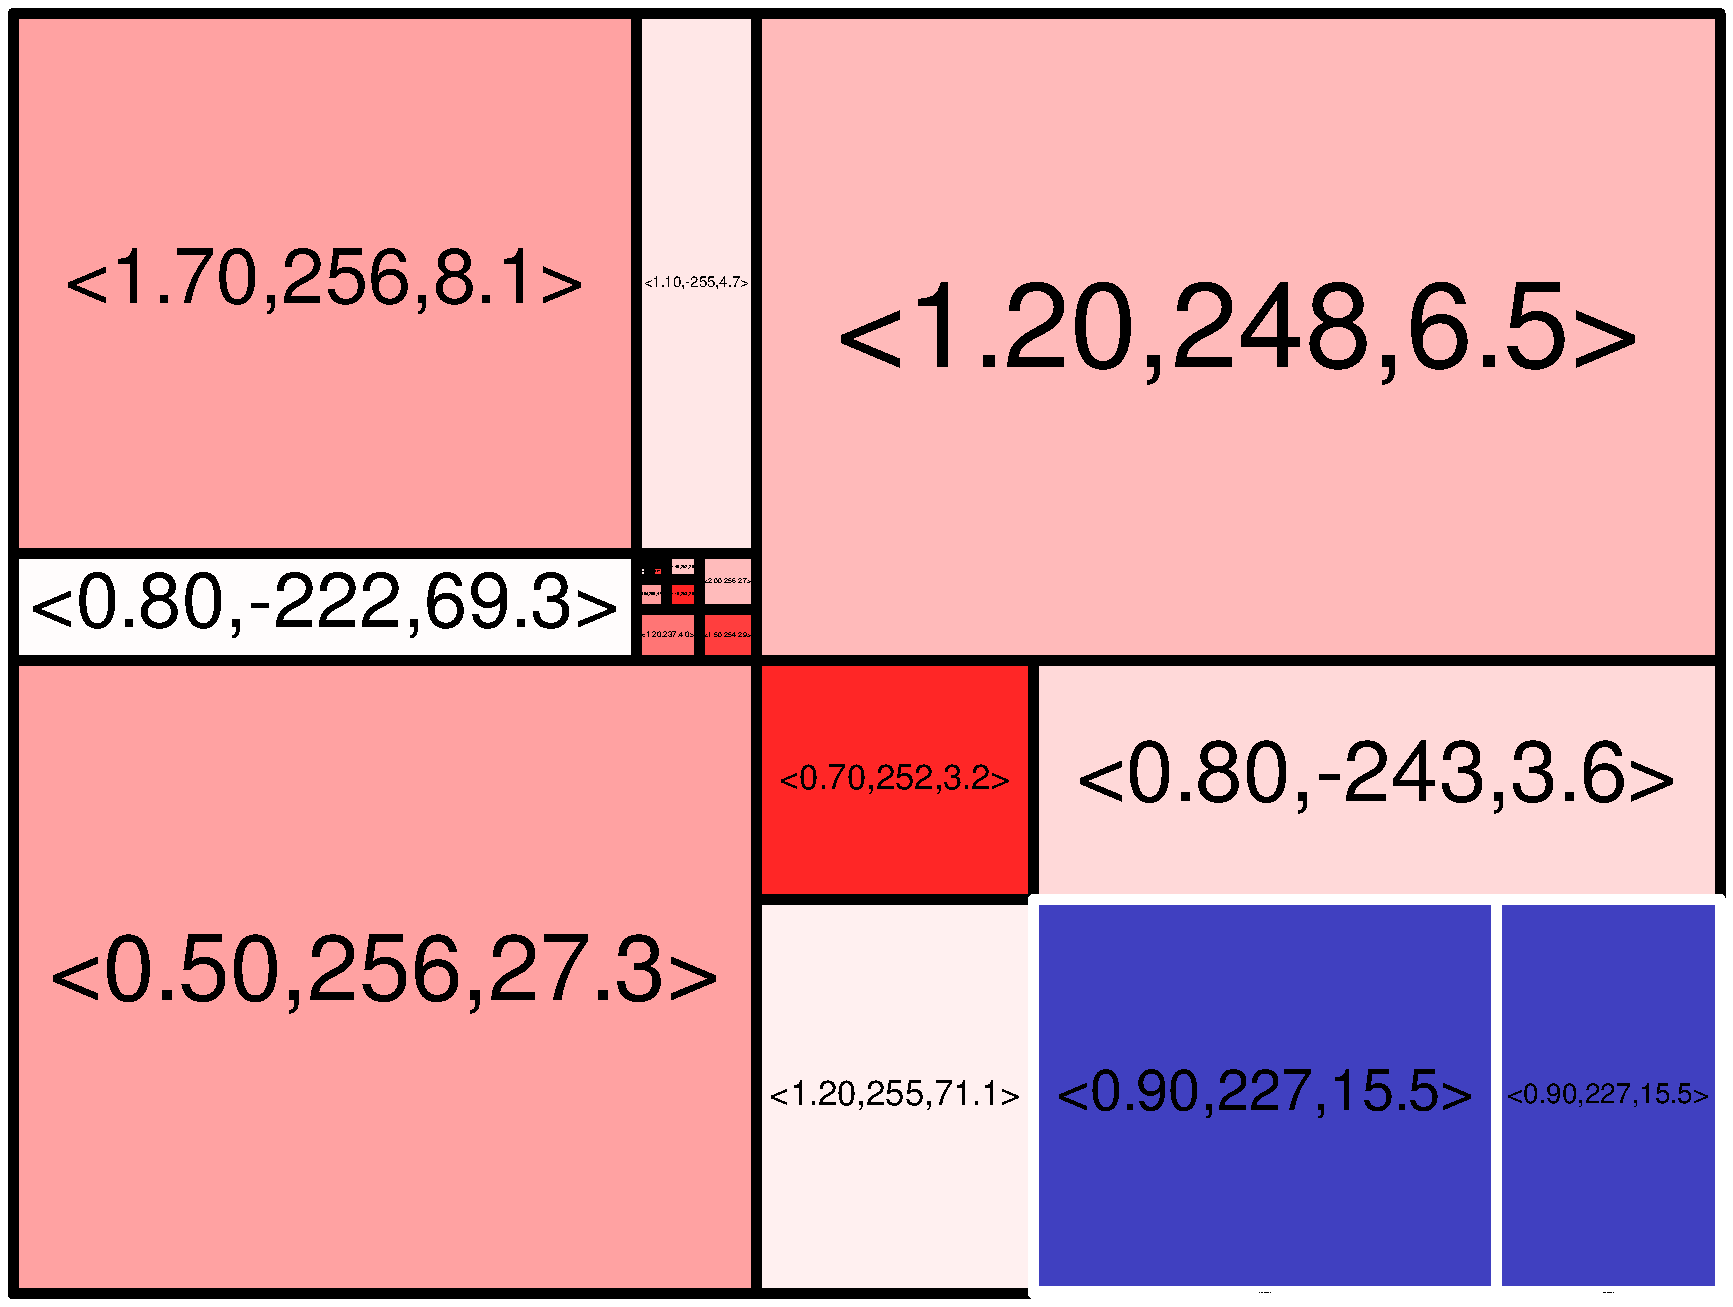
\includegraphics[width=8.5 cm]{remy-graph/graph/test20.pdf}

\end{centering}\end{frame}


\begin{frame}
\frametitle{Iterate}\begin{centering}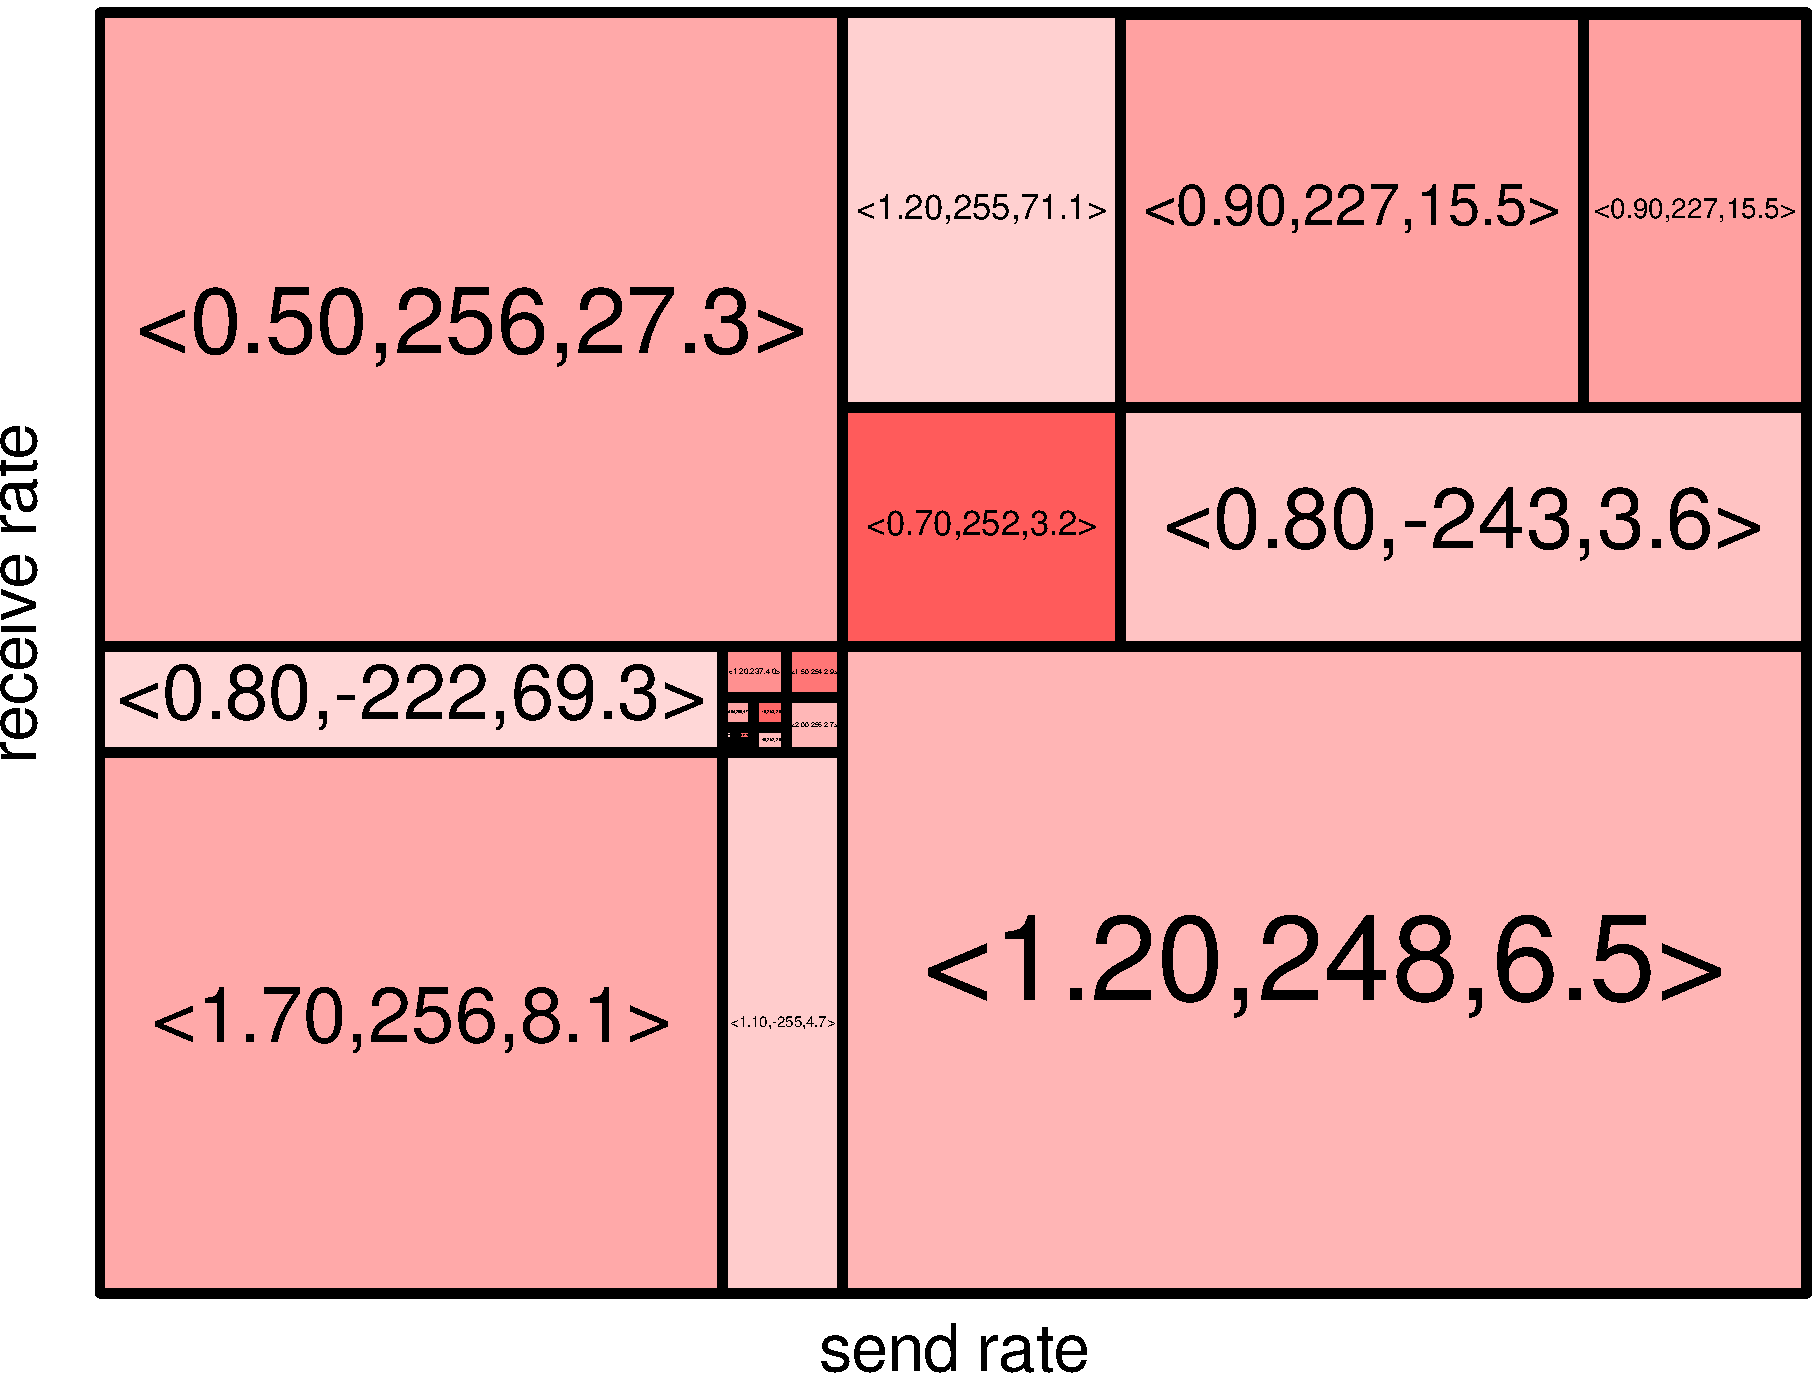
\includegraphics[width=8.5 cm]{remy-graph/graph/test21.pdf}

\end{centering}\end{frame}


\begin{frame}
\frametitle{Iterate}\begin{centering}\includegraphics[width=8.5 cm]{remy-graph/graph/test22.pdf}

\end{centering}\end{frame}


\begin{frame}
\frametitle{Iterate}\begin{centering}\includegraphics[width=8.5 cm]{remy-graph/graph/test23.pdf}

\end{centering}\end{frame}


\begin{frame}
\frametitle{Iterate}\begin{centering}\includegraphics[width=8.5 cm]{remy-graph/graph/test24.pdf}

\end{centering}\end{frame}


\begin{frame}
\frametitle{Iterate}\begin{centering}\includegraphics[width=8.5 cm]{remy-graph/graph/test25.pdf}

\end{centering}\end{frame}


\begin{frame}
\frametitle{Iterate}\begin{centering}\includegraphics[width=8.5 cm]{remy-graph/graph/test26.pdf}

\end{centering}\end{frame}


\begin{frame}
\frametitle{Iterate}\begin{centering}\includegraphics[width=8.5 cm]{remy-graph/graph/test27.pdf}

\end{centering}\end{frame}


\begin{frame}
\frametitle{Iterate}\begin{centering}\includegraphics[width=8.5 cm]{remy-graph/graph/test28.pdf}

\end{centering}\end{frame}


\begin{frame}
\frametitle{Iterate}\begin{centering}\includegraphics[width=8.5 cm]{remy-graph/graph/test29.pdf}

\end{centering}\end{frame}


\begin{frame}
\frametitle{Iterate}\begin{centering}\includegraphics[width=8.5 cm]{remy-graph/graph/test30.pdf}

\end{centering}\end{frame}


\begin{frame}
\frametitle{Iterate}\begin{centering}\includegraphics[width=8.5 cm]{remy-graph/graph/test31.pdf}

\end{centering}\end{frame}


\begin{frame}
\frametitle{Iterate}\begin{centering}\includegraphics[width=8.5 cm]{remy-graph/graph/test32.pdf}

\end{centering}\end{frame}


\begin{frame}
\frametitle{Iterate}\begin{centering}\includegraphics[width=8.5 cm]{remy-graph/graph/test33.pdf}

\end{centering}\end{frame}


\begin{frame}
\frametitle{Iterate}\begin{centering}\includegraphics[width=8.5 cm]{remy-graph/graph/test34.pdf}

\end{centering}\end{frame}


\begin{frame}
\frametitle{Iterate}\begin{centering}\includegraphics[width=8.5 cm]{remy-graph/graph/test35.pdf}

\end{centering}\end{frame}


\begin{frame}
\frametitle{Iterate}\begin{centering}\includegraphics[width=8.5 cm]{remy-graph/graph/test36.pdf}

\end{centering}\end{frame}


\begin{frame}
\frametitle{Iterate}\begin{centering}\includegraphics[width=8.5 cm]{remy-graph/graph/test37.pdf}

\end{centering}\end{frame}


\begin{frame}
\frametitle{Iterate}\begin{centering}\includegraphics[width=8.5 cm]{remy-graph/graph/test38.pdf}

\end{centering}\end{frame}


\begin{frame}
\frametitle{Iterate}\begin{centering}\includegraphics[width=8.5 cm]{remy-graph/graph/test39.pdf}

\end{centering}\end{frame}


\begin{frame}
\frametitle{Iterate}\begin{centering}\includegraphics[width=8.5 cm]{remy-graph/graph/test40.pdf}

\end{centering}\end{frame}


\begin{frame}
\frametitle{Iterate}\begin{centering}\includegraphics[width=8.5 cm]{remy-graph/graph/test41.pdf}

\end{centering}\end{frame}


\begin{frame}
\frametitle{Iterate}\begin{centering}\includegraphics[width=8.5 cm]{remy-graph/graph/test42.pdf}

\end{centering}\end{frame}


\begin{frame}
\frametitle{Iterate}\begin{centering}\includegraphics[width=8.5 cm]{remy-graph/graph/test43.pdf}

\end{centering}\end{frame}


\begin{frame}
\frametitle{Iterate}\begin{centering}\includegraphics[width=8.5 cm]{remy-graph/graph/test44.pdf}

\end{centering}\end{frame}


\begin{frame}
\frametitle{Iterate}\begin{centering}\includegraphics[width=8.5 cm]{remy-graph/graph/test45.pdf}

\end{centering}\end{frame}


\begin{frame}
\frametitle{Iterate}\begin{centering}\includegraphics[width=8.5 cm]{remy-graph/graph/test46.pdf}

\end{centering}\end{frame}


\begin{frame}
\frametitle{Iterate}\begin{centering}\includegraphics[width=8.5 cm]{remy-graph/graph/test47.pdf}

\end{centering}\end{frame}


\begin{frame}
\frametitle{Iterate}\begin{centering}\includegraphics[width=8.5 cm]{remy-graph/graph/test48.pdf}

\end{centering}\end{frame}


\begin{frame}
\frametitle{Iterate}\begin{centering}\includegraphics[width=8.5 cm]{remy-graph/graph/test49.pdf}

\end{centering}\end{frame}


\begin{frame}
\frametitle{Iterate}\begin{centering}\includegraphics[width=8.5 cm]{remy-graph/graph/test50.pdf}

\end{centering}\end{frame}


\begin{frame}
\frametitle{Iterate}\begin{centering}\includegraphics[width=8.5 cm]{remy-graph/graph/test51.pdf}

\end{centering}\end{frame}


\begin{frame}
\frametitle{Iterate}\begin{centering}\includegraphics[width=8.5 cm]{remy-graph/graph/test52.pdf}

\end{centering}\end{frame}


\begin{frame}
\frametitle{Iterate}\begin{centering}\includegraphics[width=8.5 cm]{remy-graph/graph/test53.pdf}

\end{centering}\end{frame}


\begin{frame}
\frametitle{Iterate}\begin{centering}\includegraphics[width=8.5 cm]{remy-graph/graph/test54.pdf}

\end{centering}\end{frame}


\begin{frame}
\frametitle{Iterate}\begin{centering}\includegraphics[width=8.5 cm]{remy-graph/graph/test55.pdf}

\end{centering}\end{frame}


\begin{frame}
\frametitle{Iterate}\begin{centering}\includegraphics[width=8.5 cm]{remy-graph/graph/test56.pdf}

\end{centering}\end{frame}


\begin{frame}
\frametitle{Iterate}\begin{centering}\includegraphics[width=8.5 cm]{remy-graph/graph/test57.pdf}

\end{centering}\end{frame}


\begin{frame}
\frametitle{Iterate}\begin{centering}\includegraphics[width=8.5 cm]{remy-graph/graph/test58.pdf}

\end{centering}\end{frame}


\begin{frame}
\frametitle{Iterate}\begin{centering}\includegraphics[width=8.5 cm]{remy-graph/graph/test59.pdf}

\end{centering}\end{frame}


\begin{frame}
\frametitle{Iterate}\begin{centering}\includegraphics[width=8.5 cm]{remy-graph/graph/test60.pdf}

\end{centering}\end{frame}


\begin{frame}
\frametitle{Iterate}\begin{centering}\includegraphics[width=8.5 cm]{remy-graph/graph/test61.pdf}

\end{centering}\end{frame}


\begin{frame}
\frametitle{Iterate}\begin{centering}\includegraphics[width=8.5 cm]{remy-graph/graph/test62.pdf}

\end{centering}\end{frame}


\begin{frame}
\frametitle{Iterate}\begin{centering}\includegraphics[width=8.5 cm]{remy-graph/graph/test63.pdf}

\end{centering}\end{frame}


\begin{frame}
\frametitle{Iterate}\begin{centering}\includegraphics[width=8.5 cm]{remy-graph/graph/test64.pdf}

\end{centering}\end{frame}


\begin{frame}
\frametitle{Iterate}\begin{centering}\includegraphics[width=8.5 cm]{remy-graph/graph/test65.pdf}

\end{centering}\end{frame}


\begin{frame}
\frametitle{Iterate}\begin{centering}\includegraphics[width=8.5 cm]{remy-graph/graph/test66.pdf}

\end{centering}\end{frame}


\begin{frame}
\frametitle{Iterate}\begin{centering}\includegraphics[width=8.5 cm]{remy-graph/graph/test67.pdf}

\end{centering}\end{frame}


\begin{frame}
\frametitle{Iterate}\begin{centering}\includegraphics[width=8.5 cm]{remy-graph/graph/test68.pdf}

\end{centering}\end{frame}


\begin{frame}
\frametitle{Iterate}\begin{centering}\includegraphics[width=8.5 cm]{remy-graph/graph/test69.pdf}

\end{centering}\end{frame}


\begin{frame}
\frametitle{Iterate}\begin{centering}\includegraphics[width=8.5 cm]{remy-graph/graph/test70.pdf}

\end{centering}\end{frame}


\begin{frame}
\frametitle{Iterate}\begin{centering}\includegraphics[width=8.5 cm]{remy-graph/graph/test71.pdf}

\end{centering}\end{frame}


\begin{frame}
\frametitle{Iterate}\begin{centering}\includegraphics[width=8.5 cm]{remy-graph/graph/test72.pdf}

\end{centering}\end{frame}


\begin{frame}
\frametitle{Iterate}\begin{centering}\includegraphics[width=8.5 cm]{remy-graph/graph/test73.pdf}

\end{centering}\end{frame}


\begin{frame}
\frametitle{Iterate}\begin{centering}\includegraphics[width=8.5 cm]{remy-graph/graph/test74.pdf}

\end{centering}\end{frame}


\begin{frame}
\frametitle{Iterate}\begin{centering}\includegraphics[width=8.5 cm]{remy-graph/graph/test75.pdf}

\end{centering}\end{frame}


\begin{frame}
\frametitle{Iterate}\begin{centering}\includegraphics[width=8.5 cm]{remy-graph/graph/test76.pdf}

\end{centering}\end{frame}


\begin{frame}
\frametitle{Iterate}\begin{centering}\includegraphics[width=8.5 cm]{remy-graph/graph/test77.pdf}

\end{centering}\end{frame}


\begin{frame}
\frametitle{Iterate}\begin{centering}\includegraphics[width=8.5 cm]{remy-graph/graph/test78.pdf}

\end{centering}\end{frame}


\begin{frame}
\frametitle{Iterate}\begin{centering}\includegraphics[width=8.5 cm]{remy-graph/graph/test79.pdf}

\end{centering}\end{frame}


\begin{frame}
\frametitle{Iterate}\begin{centering}\includegraphics[width=8.5 cm]{remy-graph/graph/test80.pdf}

\end{centering}\end{frame}


\begin{frame}
\frametitle{Iterate}\begin{centering}\includegraphics[width=8.5 cm]{remy-graph/graph/test81.pdf}

\end{centering}\end{frame}


\begin{frame}
\frametitle{Iterate}\begin{centering}\includegraphics[width=8.5 cm]{remy-graph/graph/test82.pdf}

\end{centering}\end{frame}


\begin{frame}
\frametitle{Iterate\hspace{10 cm}.}\begin{centering}\includegraphics[width=8.5 cm]{remy-graph/graph/test83.pdf}

\end{centering}\end{frame}


\begin{frame}
\frametitle{Iterate\hspace{10 cm}.}\begin{centering}\includegraphics[width=8.5 cm]{remy-graph/graph/test84.pdf}

\end{centering}\end{frame}


\begin{frame}
\frametitle{Iterate\hspace{10 cm}.}\begin{centering}\includegraphics[width=8.5 cm]{remy-graph/graph/test85.pdf}

\end{centering}\end{frame}


\begin{frame}
\frametitle{Iterate}\begin{centering}\includegraphics[width=8.5 cm]{remy-graph/graph/test86.pdf}

\end{centering}\end{frame}


\begin{frame}
\frametitle{Iterate\hspace{10 cm}*}\begin{centering}\includegraphics[width=8.5 cm]{remy-graph/graph/test87.pdf}

\end{centering}\end{frame}


\begin{frame}
\frametitle{Iterate}\begin{centering}\includegraphics[width=8.5 cm]{remy-graph/graph/test88.pdf}

\end{centering}\end{frame}


\begin{frame}
\frametitle{Evaluation in ns-2}

\section{Evaluation}

\begin{itemize}

\item End-to-end comparators: \textcolor{Red}{NewReno, Cubic, Compound, Vegas}

\item In-net comparators: \textcolor{DarkGreen}{Cubic-over-sfqCoDel, XCP}

\item Simulation setup published for replication

\end{itemize}

\begin{centering}
\includegraphics[width=9 cm]{reproducethis.png}

\end{centering}

\end{frame}

\begin{frame}
\frametitle{Scenario 1: fixed-rate network, homogenous senders}

\includegraphics[width=\textwidth]{dumbbell.pdf}

\end{frame}

\begin{frame}
\frametitle{Scenario 1: model \& mission}

\begin{tabular}{lllll}
\bf Quantity & & \bf Simulation parameter & \bf Remy \textcolor{DarkBlue}{model} \\

\hline Link speed & & 15~Mbps & Uniform(10, 20)~Mbps \\

RTT & & 150~ms & Uniform(100, 200)~ms \\

$n$ & & 8 & Uniform(1, 16) \\

``On'' process & & $\mathrm{exp}[\mu = 100]\,\textbf{\textcolor{DarkBlue}{kB}}$ & $\mathrm{exp}[\mu = 5]\,\textbf{\textcolor{DarkBlue}{s}}$ \\

``Off'' process & & $\mathrm{exp}\left[\mu = \textcolor{DarkBlue}{\bm {\frac{1}{2}}}\right]\,\textsf{s}$ & $\mathrm{exp}[\mu = \textcolor{DarkBlue}{\bm 5} ]\,\textsf{s}$ \\

\end{tabular}

\ssline
\ssline

\textbf{Remy \textcolor{DarkGreen}{missions}:} \[\sum_i \log \left[ \frac{\textsf{throughput}_i}{\big(\textsf{delay}_i\big)^{\textcolor{DarkBlue}{{\bm \delta}}}} \right]\]

\[\textcolor{DarkBlue}{{\bm \delta}} \in \bigg\{ \frac{1}{10}, 1, 10 \bigg\} \]

\end{frame}

\begin{frame}
\frametitle{Scenario 1: throughput-delay plot}

\begin{centering}
\only<1>{\includegraphics[width=8.5 cm]{eth8-annotated-11.pdf}}\only<2>{\includegraphics[width=8.5 cm]{eth8-annotated-10.pdf}}\only<3>{\includegraphics[width=8.5 cm]{eth8-annotated-9.pdf}}\only<4>{\includegraphics[width=8.5 cm]{eth8-annotated-8.pdf}}\only<5>{\includegraphics[width=8.5 cm]{eth8-annotated-7.pdf}}\only<6>{\includegraphics[width=8.5 cm]{eth8-annotated-6.pdf}}\only<7>{\includegraphics[width=8.5 cm]{eth8-annotated-7.pdf}}\only<8>{\includegraphics[width=8.5 cm]{eth8-annotated-5.pdf}}\only<9>{\includegraphics[width=8.5 cm]{eth8-annotated-4.pdf}}\only<10>{\includegraphics[width=8.5 cm]{eth8-annotated-3.pdf}}\only<11>{\includegraphics[width=8.5 cm]{eth8-annotated-1.pdf}}\only<12>{\includegraphics[width=8.5 cm]{eth8-annotated.pdf}}

\end{centering}
\end{frame}

%\begin{frame}
%\frametitle{Scenario 2: $n = 12$, heavy-tailed flow lengths}
%
%\begin{centering}
%\includegraphics[width=8.5 cm]{eth12-final-flowcdf.pdf}
%
%\end{centering}
%
%\end{frame}

\begin{comment}
\begin{frame}
\frametitle{Scenario 2: Verizon LTE, $n = 8$}

\begin{centering}
\includegraphics[width=8.5 cm]{vzw-8-final.pdf}

\end{centering}
\end{frame}
\end{comment}

\begin{frame}
\frametitle{The effect of prior knowledge}

\begin{centering}

\noindent \only<1>{\includegraphics[width=3.1 in]{oprange-1.pdf}}\only<2>{\includegraphics[width=3.1 in]{oprange-2.pdf}}\only<3>{\includegraphics[width=3.1 in]{oprange-3.pdf}}\only<4>{\includegraphics[width=3.1 in]{oprange-4.pdf}}\only<5>{\includegraphics[width=3.1 in]{oprange-5.pdf}}\only<6>{\includegraphics[width=3.1 in]{oprange-6.pdf}}\only<7>{\includegraphics[width=3.1 in]{oprange-all.pdf}}

\end{centering}

\end{frame}

\begin{frame}
\frametitle{Safety and effectiveness of congestion control}

\Large

What is safety?

\begin{itemize}

\item Bound \textbf{worst-case} performance
  
\item System always converges to cycle

\item Quick convergence time

\item Can we verify this programmatically?

\end{itemize}

\end{frame}

\begin{frame}

\includegraphics[width=\textwidth]{absolute-intersend-plot.pdf}

\end{frame}

\begin{frame}
\frametitle{Formalizing systems design}

\section{Big picture?}

\begin{itemize}
 
\item Many design choices represent a tradeoff

\item[]

\item \emph{``Which choice did we make?''}

\item[]

\item \emph{``What were the alternatives?''}

\end{itemize}
\end{frame}

\begin{frame}
\frametitle{Human-designed congestion control, Stanford CS244}

\begin{itemize}
\item A.~Sivaraman and I developed a rate-control scheme for cellular networks (NSDI '13)

\item[]

\item Alterman \& Quach reproduced some of our measurements

\item[]

\item {\scriptsize\texttt{http://ReproducingNetworkResearch.wordpress.com/2013/03/12/1216/}}

\item[]

\item Won best project award in Stanford CS244 (March 2013)!

\end{itemize}

\end{frame}

\begin{frame}
\frametitle{M.I.T.~6.829 contest (March--April 2013)}

\begin{itemize}
\item Turnkey network emulator, evaluation

\item Sender, receiver run in Linux containers

\item 4th prize: \$20

\item 3rd prize: \$30

\item 2nd prize: \$40

\item (If beat Sprout) 1st prize: \pause {\color{DarkBlue}{\bf Co-authorship on future paper}}

\end{itemize}

\vspace{\baselineskip}
\vspace{\baselineskip}
\vspace{\baselineskip}

\visible<3>{\scriptsize Anirudh Sivaraman, KW, Pauline Varley, Somak
  Das, Joshua Ma, Ameesh Goyal, Jo\~{a}o Batalha, and Hari Balakrishnan,
  \textbf{Protocol Design Contests}, \textit{Computer Communications Review} (July 2014)}

\end{frame}

\begin{frame}
\frametitle{Baseline}

\begin{centering}
\includegraphics[width=0.9\columnwidth]{pointplot-nostudents.png}

\end{centering}

\end{frame}

\begin{frame}
\frametitle{Land of 3,000 student protocols}

\begin{centering}
\includegraphics[width=0.9\columnwidth]{pointplot.png}

\end{centering}

\end{frame}

\begin{frame}
\frametitle{Sprout is on the frontier}

\begin{centering}
\includegraphics[width=0.9\columnwidth]{pointplot-withhull.png}

\end{centering}

\end{frame}

%\begin{frame}
%  \frametitle{Alternate Remy: MIT students}
%
%\begin{centering}
%\only<1>{\includegraphics[width=0.9\textwidth]{pointplot-withhull-nosprout-minus4.pdf}}\only<2>{\includegraphics[width=0.9\textwidth]{pointplot-withhull-nosprout-minus3.pdf}}\only<3>{\includegraphics[width=0.9\textwidth]{pointplot-withhull-nosprout-minus2.pdf}}\only<4>{\includegraphics[width=0.9\textwidth]{pointplot-withhull-nosprout-minus1.pdf}}\only<5>{\includegraphics[width=0.9\textwidth]{pointplot-withhull-nosprout.pdf}}\only<6>{\includegraphics[width=0.9\textwidth]{pointplot-withhull.pdf}}
%
%\end{centering}
%
%\end{frame}

%\begin{frame}
%\frametitle{Future work}
%
%\section{Discussion}
%
%\begin{itemize}
%\item Real-time implementation
%
%\item[]
%
%\item Is there an ``operating range-performance'' product?
%
%\item[]
%
%\item What is the value of different congestion signals?
%
%\item[]
%
%\item What is the cost of TCP-friendliness?
%
%\end{itemize}
%
%\end{frame}

%\begin{frame}
%\frametitle{Surprises}
%
%\LARGE
%
%\begin{itemize}
%
%\item \textcolor{DarkGreen}{Computer-designed} {\LARGE \textbf{\textgreater}} \textcolor{DarkRed}{human-designed}
%
%\item[]
%
%\item \textcolor{DarkGreen}{End-to-end} {\LARGE \textbf{\textgreater}} \textcolor{DarkRed}{in-network{\LARGE \textbf{*}}}
%
%\item[]
%
%\item[] \hspace{6.0 cm}\normalsize\textcolor{DarkRed}{{\bf *} (so far)}
%
%\end{itemize}
%
%\end{frame}
%
%\begin{frame}
%\frametitle{Acknowledgments}
%
%\begin{centering}
%\begin{tabular}{lll}
%Anirudh Sivaraman & Ranjita Bhagwan \\
%Leslie Kaelbling & Christopher Amato \\
%Scott Shenker & Frans Kaashoek \\
%Nickolai Zeldovich & Damon Wischik \\
%Chris Lesniewski & Juliusz Chroboczek \\
%\end{tabular}
%
%\end{centering}
%
%\ssline
%\ssline
%
%\footnotesize We thank the members of the MIT Center for Wireless
%Networks and Mobile Computing (Wireless@MIT), including Amazon.com,
%Cisco, Google, Intel, Mediatek, Microsoft, ST Microelectronics, and
%Telefonica, for their support. KW was supported by the Claude
%E.~Shannon Research Assistantship. This work was also supported in
%part by NSF grant CNS-1040072.
%
%\end{frame}

\begin{frame}
\frametitle{New tradeoffs}

\large

\begin{itemize}

\item Traditionally: simple rules, complex behavior

\item With Remy: complex rules, consistent behavior

\item[]

\item \textcolor{DarkGreen}{Computer-designed} {\LARGE \textbf{\textgreater}} \textcolor{Red}{human-designed}

\item \textcolor{DarkGreen}{End-to-end} {\LARGE \textbf{\textgreater}} \textcolor{Red}{in-network}

\item[]

\item The network evolves. Transport should let it!

\end{itemize}

\end{frame}

\begin{comment}
\begin{frame}
  \frametitle{New projects}

\large
  
\begin{itemize}

\item \textbf{\textcolor{DarkBlue}{Mahimahi}}: composable network emulator containers

\item[]
  
\item \textbf{\textcolor{DarkBlue}{Cloud Query Planner}}

\item[]
  
\item \textbf{\textcolor{DarkBlue}{Alfalfa}}: continuation-based streaming video

\item[]
  
\item \textbf{\textcolor{DarkBlue}{Self-Incentivizing Networks}}

  \end{itemize}
\end{frame}

\begin{frame}

\LARGE
  
\begin{centering}
  
  [mahimahi demo]

\end{centering}

\end{frame}

\begin{frame}
  \frametitle{Cloud Query Planner}

  \large

  \begin{itemize}
    \item Idea: solve \textcolor{DarkBlue}{problems}, not \textcolor{Maroon}{workloads}

    \item[]

    \item Library of solvers for heterogenous datacenters

    \item[]

    \item Example problem: GraySort benchmark.

    \item[]

    \item Several strategies to compromise upfront time vs.~query perf.~vs.~money
  \end{itemize}
\end{frame}

\begin{frame}
\frametitle{Proposal: understand and expose the tradeoffs}
  
\includegraphics[width=0.7 \textwidth]{sliders.png}

\end{frame}

\begin{frame}
\frametitle{Model and reality}

\Large

  \begin{itemize}
  \item \textcolor{DarkBlue}{\bf Model} informs \textcolor{DarkBlue}{\bf reality}: recommends strategies based on performance/cost predictions.

    \item[]
    
    \item \textcolor{DarkBlue}{\bf Reality} informs \textcolor{DarkBlue}{\bf model}: learns constants that drive model predictions.
  \end{itemize}
  
\end{frame}

\begin{frame}
\frametitle{Alfalfa}

\large

\begin{itemize}

\item Problem: streaming video wastes \~{}1 Mbps because user \emph{might} need to seek

\item[]
  
\item Solution: understand the video decoder and encode continuations

\item[]
  
\item Benefits: instant edits, progressive pause, fast seeks

\item[]

\item ``World Wide Web of Video''

\item[]

\item Live TV test project

\end{itemize}
  
\end{frame}

\begin{frame}
\frametitle{Self-incentivizing networks}

\large

\begin{itemize}

\item Anybody can add incremental capacity to network

\item Be rewarded for contribution

\item Every packet scheduled ``rationally''

\pause

\item[]

\item \textcolor{DarkRed}{\textbf{\sout{TCP}}}

\pause

\item \textcolor{DarkRed}{\textbf{\sout{BGP}}}

  \pause
  
\item \textcolor{DarkRed}{\textbf{\sout{AQM}}}  

\pause

\item \textcolor{DarkRed}{\textbf{\sout{95th-percentile 5-minute window in a month}}}
\item \textcolor{DarkRed}{\textbf{\sout{lawyers}}}

\end{itemize}

\end{frame}

\begin{frame}
  \frametitle{SIN deployments?}

\Large
  
  \begin{itemize}
  \item Neighbor sharing

    \item[]
    
  \item Caltrain

    \item[]
    
  \item Urban mesh network
  \end{itemize}
\end{frame}

\end{comment}

\begin{frame}
  
\frametitle{Systems ex Machina}

\begin{itemize}

\item In systems design, \textbf{\textcolor{DarkBlue}{showing our
    work}$^{*}$} yields better performance, and frees adjacent systems
to evolve.

\item[] \textcolor{DarkBlue}{\textbf{*} (clearly enough for a computer to recreate the design)}

\end{itemize}

\vspace{\baselineskip}

\begin{centering}
keithw@cs.stanford.edu

\vspace{7 pt}

\textcolor{DarkBlue}{https://cs.stanford.edu/~keithw}

\vspace{\baselineskip}

\includegraphics[width=1.5 cm]{stanford-tree.jpg}

\end{centering}

\end{frame}

\begin{frame}

  \LARGE

\begin{centering}
  
  [backup slides]

\end{centering}
  
\end{frame}

\begin{frame}
\frametitle{RemyCC competing against itself}

\begin{centering}

\noindent \only<1>{\includegraphics[width=3.3 in]{homo-1.pdf}}\only<2>{\includegraphics[width=3.3 in]{homo-2.pdf}}\only<3>{\includegraphics[width=3.3 in]{homo-3.pdf}}

\end{centering}

\end{frame}

\begin{frame}
\frametitle{RemyCC competing against TCP NewReno}

\begin{centering}

\noindent \only<1>{\includegraphics[width=3.3 in]{hetero-1.pdf}}\only<2>{\includegraphics[width=3.3 in]{hetero-2.pdf}}\only<3>{\includegraphics[width=3.3 in]{hetero-3.pdf}}

\end{centering}

\end{frame}

\begin{frame}
\frametitle{When the model is wrong about the topology}

\large

\begin{centering}
\textcolor{DarkBlue}{\only<1>{One bottleneck}\only<2>{Two bottlenecks}}

\end{centering}

\vspace{\baselineskip}
\vspace{\baselineskip}

\only<1>{\includegraphics[width=\textwidth]{onelink.pdf}}\only<2>{\includegraphics[width=\textwidth]{twolink.pdf}}

\end{frame}

\begin{frame}

\begin{centering}
\frametitle{When the model is wrong about the topology}

\noindent \only<1>{\includegraphics[width=3.4 in]{multilink-5.pdf}}\only<2>{\includegraphics[width=3.4 in]{multilink-4.pdf}}\only<3>{\includegraphics[width=3.4 in]{multilink-3.pdf}}\only<4>{\includegraphics[width=3.4 in]{multilink-all.pdf}}

\end{centering}

\end{frame}

\end{document}
